\documentclass[10pt,fleqn]{report}

\usepackage[english]{babel}
\usepackage[utf8x]{inputenc}
\usepackage{enumerate}
\usepackage{amsmath}
\usepackage{amssymb}
\usepackage{amsfonts}
\usepackage{mathtools}
\usepackage{graphicx}
\usepackage{bm}
\usepackage[usenames,dvipsnames]{color}
\usepackage{todonotes}
\usepackage{dsfont}
\usepackage{hyperref}
\hypersetup{
    colorlinks,
    citecolor=black,
    filecolor=black,
    linkcolor=black,
    urlcolor=black
}
\usepackage{algorithm}
\usepackage{algorithmic}
\usepackage{appendix}
\usepackage{caption}
\usepackage{subcaption}
\usepackage{fancyvrb}
\usepackage{subfigure}
\usepackage{graphicx,xcolor}
\usepackage{pifont,mdframed}
\usepackage{tikz}
\usetikzlibrary{fit,positioning}
\usepackage{setspace}
\onehalfspacing


\newcommand{\specialcell}[2][c]{%
  \begin{tabular}[#1]{@{}c@{}}#2\end{tabular}}

\newcommand \etr[0] {
    \text{etr}
}

\newcommand \Etr[1] {
    \text{etr}\left( { #1 } \right)
}

\newcommand \tinymath[1] {{  \mbox{\tiny ${#1}$ }  }}

%
% Macros
%
\newcommand \cashort[1] { {\todo[color=yello]{#1 -- Cedric}} }
\newcommand \calong[1]  { { \todo[inline,color=yellow]{#1 -- Cedric} } }
\newcommand \gbshort[1] { {\todo[color=cyan!40]{#1 -- Guillaume}} }
\newcommand \gblong[1]  { { \todo[inline, color=cyan!40]{#1 -- Guillaume} } }
\newcommand \mgshort[1] { {\todo{#1 -- Mark}} }
\newcommand \mglong[1]  { { \todo[inline]{#1 -- Mark} } }
\newcommand \bfshort[1] { {\todo[color=green!40]{#1 -- Bryan}} }
\newcommand \bflong[1]  { { \todo[inline,color=green!40]{#1 -- Bryan} } }


% Adds a plus const to the end of a math expression
\def \pcst{+\text{const}}

% A fancy version for capital R
\def \Rcal{\mathcal{R}}

% A fancy version for r
\def \rcal{\mathbf{r}}

% Loss function / log likelihood as appropriate
\def \L{\mathcal{L}}

% KL divergence [Math Mode]
\newcommand{\kl}[2] {
	\text{KL}\left[#1||#2\right]
}

\newcommand{\symmkl}[2] {
	\text{KL}^{symm}\left[#1||#2\right]
}

\newcommand \vecf[1] {
    \text{vec}\left(#1\right)
}

\newcommand \ent[1] {
    \text{H} \left[ #1 \right]
}

\newcommand \mut[2] {
    \text{I} \left[ #1 ; #2 \right]
}

\newcommand \dvi[2] {
    \text{D}_\text{VI} \left[ #1; #2 \right]
}

% Starts an expected value expresses [Math Mode]
\newcommand{\starte}[1] {%
	\mathbb{E}_{#1}\left[
}

% Ends an expected value expression [Math Mode]
\def \ende{\right]}

% Starts an varianc expresses [Math Mode]
\newcommand{\startv}[1] {%
	\mathbb{V}\text{ar}_{#1}\left[
}

% Ends an variance expression [Math Mode]
\def \endv{\right]}

%\newcommand \ex[2] {
%    \bigl\langle #1 \bigr\rangle_{#2}
%}
\newcommand \ex[2] {
    \mathbb{E}_{ { #2 } }\left[ #1 \right]
}
\newcommand \var[2] {
    \mathbb{V}\text{ar}_{ { #2 } }\left[ #1 \right]
}
\newcommand \cov[1] {
    \mathbb{C}\text{ov}[ #1 ]
}

\newcommand \halve[1] {
	\frac{#1}{2}
}

\newcommand \half {
    \halve{1}
}

\newcommand \tr { \text{tr} }

\newcommand \T { ^\top }

\newcommand \fixme[1] {
    {\color{red} FIXME: #1}
}

\newcommand \vv[1] { \bm #1 }

\newcommand{\mbeq}{\overset{!}{=}}

\def\app#1#2{%
  \mathrel{%
    \setbox0=\hbox{$#1\sim$}%
    \setbox2=\hbox{%
      \rlap{\hbox{$#1\propto$}}%
      \lower1.1\ht0\box0%
    }%
    \raise0.25\ht2\box2%
  }%
}
\def\approxpropto{\mathpalette\app\relax}

\newcommand \diag[1] { \text{diag} \left( {#1} \right) }
\newcommand \diagonal[1] { \text{diagonal} \left( {#1} \right) }

\newcommand \Ed {{ \vv{\xi}_d}}
\newcommand \Edj {{\xi_{dj}}}
\newcommand \Edk {{\xi_{dk}}}
\newcommand \AEdj {{\Lambda(\xi_{dj})}}
\newcommand \AEdk {{\Lambda(\xi_{dk})}}
\newcommand \AEd  {{ \bm{\Lambda}(\bm{\xi}_d) }}

\newcommand \Axi { { \Lambda_{\xi} } }
\newcommand \bxi { { \vv{b}_{\xi} } }
\newcommand \cxi { { c_{\xi} } }


\newcommand \wdoc      { { \vv{w}_d } }
\newcommand \wdt[0]  { { w_{dt} } }
\newcommand \wdn[0]  { { \vv{w}_{dn} } }
\newcommand \wdnt[0]  { { w_{dnt} } }
\newcommand \wdd[0]   { { \vv w_{d} } }
\newcommand \zd[0]   { { \vv z_{d} } }
\newcommand \zdn[0]  { { \vv{z}_{dn} } }
\newcommand \zdnk[0] { { z_{dnk} } }
\newcommand \zdk[0]  { { z_{dk} } }
\newcommand \thd[0]  { { \vv \theta_d } }
\newcommand \thdk[0] { { \theta_{dk} } }
\newcommand \thdj[0] { { \theta_{dj} } }
\newcommand \epow[1] { { e^{#1} } }
\newcommand \pkt     { { \phi_{kt}  } }
\newcommand \pk      { { \vv \phi_k } }
\newcommand \lmd     { { \vv \lambda_d } }
\newcommand \lmdk    { { \lambda_{dk} } }
\newcommand \xd      { { \vv x_d } }
\newcommand \atxd     { A ^\top \bm x_d}
\newcommand \axd     { A\bm x_d}
\newcommand \tsq      { { \tau^2 } }
\newcommand \ssq      { { \sigma^2 } }
\newcommand \tmsq     { { \tau^{-2} } }
\newcommand \asq      { { \alpha^2 } }
\newcommand \amsq     { { \alpha^{-2} } }
\newcommand \sgsq     { { \sigma^2 } }
\newcommand \xvec     { { \vv{x} } }
\newcommand \omk      { { \bm \omega _k } }
\newcommand \omkt     { { \omega_{kt} } }
\newcommand \oma     { { \Omega_A } }
\newcommand \gdn      { { \vv{\gamma}_{dn} } }
\newcommand \gdnk     { { \gamma_{dnk} } }
\newcommand \gdk      { { \gamma_{dk} } }
\newcommand \isigt   { { \Sigma^{-1}_{\bm \theta} } }

\newcommand \nd { { n_{d\cdot\cdot} } }


\newcommand \halfSig { \frac{1}{2\sigma^2} }

\newcommand \cat[1]   { \mathcal{C} \left( {#1} \right) }
\newcommand \nor[2]   { \mathcal{N} \left( {#1}, {#2} \right) }
\newcommand \nord[3]   { \mathcal{N}_{#1} \left( {#2}, {#3} \right) }
\newcommand \mnor[3]  { \mathcal{N} \left(#1, #2, #3\right) }
\newcommand \norp[3]  { \mathcal{N} \left(#1; #2, #3\right) }
\newcommand \mnorp[4] { \mathcal{N} \left(#1; #2, #3, #4\right) }
\newcommand \mul[1]   { \mathcal{M} \left( {#1} \right) }
\newcommand \muln[2]  { \mathcal{M} \left( {#1},{#2} \right) }
\newcommand \dir[1]   { \mathcal{D} \left( {#1} \right) }
\newcommand \pois[1]  { \mathcal{P} \left( {#1} \right) }
\newcommand \gp[2]    { \mathcal{GP} \left( {#1}, #2 \right) }
\newcommand \dir[1]   { \mathcal{D} \left( {#1} \right) }
\newcommand \gam[2]   { \Gamma \left( {#1}, {#2} \right) }
\newcommand \betadist[2]  { Beta \left( {#1}, {#2} \right) }
\newcommand \DP[1]    { \text{DP} \left( {#1} \right) }
\newcommand \PYP[1]   { \text{PYP} \left( {#1} \right) }
\newcommand \GP[2]    { \text{GP} \left( {#1}, {#2} \right) }

\newcommand \lne[1]  { { \ln \left( 1 + e^{ #1 } \right) } }
\newcommand \Tr[1]   { \tr \left(  {#1}  \right) }

\newcommand \roud  { \vv{\rho}_{d}  }
\newcommand \rodk { \rho_{dk} }

\newcommand \exA[1]  { \ex{#1}{q(A)} }
\newcommand \exV[1]  { \ex{#1}{q(V)} }
\newcommand \exT[1]  { \ex{#1}{q(\Theta)} }
\newcommand \extd[1] { \ex{#1}{q(\thd)} }
\newcommand \exTV[1] { \ex{#1}{q(\Theta)q(V)} }

\newcommand \Real[0]  { { \mathbb{R} } }
\newcommand \VReal[1] { { \mathbb{R}^{#1} } }
\newcommand \MReal[2] { { \mathbb{R}^{#1 \times #2} } }
\newcommand \Nat[0]  { { \mathbb{N} } }
\newcommand \VNat[1] { { \mathbb{N}^{#1} } }
\newcommand \MNat[2] { { \mathbb{N}^{#1 \times #2} } }

\newcommand \inv[1] { {#1}^{-1} }
\newcommand \invb[1] { \inv{\left( #1 \right)} }

\newcommand \cn { \textsuperscript{\texttt{[{\color{blue}Citation Needed}]}} }

\newcommand \const { { \text{c} } }

\providecommand \floor [1] { \left \lfloor #1 \right \rfloor }
\providecommand \ceil [1] { \left \lceil #1 \right \rceil }


\newcommand \vt[2] { { #1^{(#2)} } }

\newcommand \hashtag[1] { { \ttfamily \##1 } }

\newcommand \mvy  { \vv{m}_{\vv{y}} }
\newcommand \sigvy { { S_Y } }

\newcommand \mmy  { M_Y      }
\newcommand \md   { \vv{m}_d }
\newcommand \phin { \vv{\phi}_n }
\newcommand \isigma { { \inv{\Sigma} } }

\newcommand \sigv     { { \Sigma_V } }
\newcommand \isigv     { { \Sigma^{-1}_V } }

\newcommand \sigy { { \Sigma_Y } }
\newcommand \isigy { { \Sigma_{-1}_Y } }


\newcommand \omy  { { \Omega_Y } }
\newcommand \iomy { { \inv{\Omega_Y} } }

\newcommand \siga     { { \Sigma_A } }
\newcommand \isiga     { { \Sigma^{-1}_A } }
\newcommand \diagv { { \diag{\nu_1,\ldots,\nu_P} } }

\newcommand \ma { \vv{m}_a }
\newcommand \my { \vv{m}_y }

\newcommand \VoU { V \otimes U }

%\newcommand \one { \mathbb{1} }
\newcommand \one  {{  \mathds{1} }}

\newcommand \lse { \text{lse} }
%\newcommand \lse[0] { \mathrm{lse} }

% Conditional independence
\def\ci{\perp\!\!\!\perp} % from Wikipedia



% ------ For the eval section

% Multinomial PDF [Math Mode]
% params: 1 - the variable
%         2 - the value
%         3 - the state indicator (e.g. k for a distro with K values)
%         4 - any additional subscript
\newcommand{\mpdf}[4] {
	\prod_{#3} {#1}_{{#4} {#3}} ^ {#2}
}

% Dirichlet PDF [Math Mode]
% params: 1 - the variable
%         2 - the hyper-parameter
%         3 - the state indicator (e.g. k for a distro with K values)
%         4 - any additional subscript
\newcommand{\dpdf}[4] {
	\frac{1}{B({#2})} \prod_{#3} {#1}_{{#4} {#3}} ^ {({#2}_{#3} - 1)}
}

% To simplify the sampling equations, this is indicates
% that the given value has had datapoint "m" stripped out
%
\newcommand{\lm}[1] {
	#1^{\setminus m}
}

\newcommand \model[0] {
    \mathcal{M}
}

\newcommand \perplexity[1] {
    \mathcal{P} \left( { #1 } \right)
}

\newcommand \WTrain {
    \mathcal{W}^{(t)}
}

\newcommand \WQuery {
    \mathcal{W}^{(q)}
}

\newcommand \oneover[1] {
    \frac{1}{ {#1} }
}

\newcommand \samp[1] {
    { #1 }^{(s)}
}

\newcommand \etd[0] {
    \vv{\eta}_d
}

\begin{document}

%\title{Correlated Admixtures of Text Conditioned On Arbitrary Features}
%\author{Bryan Feeney}
%\maketitle
%{\centering \textsc
%A dissertation
%submitted to the department of physics
%and the committee on graduate studies
%of University College London
%in partial fulfilment of the requirements
%for the degree of
%doctor of philosophy}
 
%titlepage
\thispagestyle{empty}
\begin{center}
\begin{minipage}{0.75\linewidth}
    \centering
%University logo
    %\includegraphics[width=0.3\linewidth]{logo.pdf}
    %\rule{0.4\linewidth}{0.15\linewidth}\par
    \vspace{3cm}
%Thesis title
    {\uppercase{\Large Correlated Admixture Models of Text Conditioned on Arbitrary Features\par}}
    \vspace{3cm}
%Author's name
    {\Large Bryan Feeney\par}
    \vspace{3cm}
%Degree
    {\Large A thesis submitted to the Department of Statistics Science and the Committee on Graduate Studies of University College London in partial fulfilment of the degree of Doctor of Philosophy\par}
    \vspace{3cm}
%Date
    {\Large September 2017}
\end{minipage}
\end{center}
\clearpage
\begin{abstract}
This body of research is concerned with the use of admixture models for heterogeneous features. In particular it focuses on the case where text is paired with other observations, and seeks to either use those observations to better explain the text, model those observations alongside text, in particular the case where such features are partially observed, and combinations of the two.

Admixture models of text, more commonly known as topic-models, have been the dominant method for modelling textual corpora since the publication of the Latent Dirichlet Analysis algorithm\cite{BleiNgJordan2003}, however with the exception of Supervised LDA\cite{Blei2008} and Dirichlet Multinomial Regression\cite{Mimno2008}, most methods for dealing with hetereogenous datasets have been ad hoc and not generalisable.

We seek to extend this, by deriving novel methods for the incorporation of additional observations into topic models in a generic, widely applicable form. In particular, we seek to use techniques from the field of multi-task learning to improve the predictive power of these methods. We focus on the use of matrix-variate priors, and non-conjugate Bayesian Inference, to derive Bayesian methods for the incorporation of observed features in topic models which can capture task, i.e. topic, correlations.

The first contribution arising from this focus is a method for modelling very ``micro-texts", i.e. documents whose average length is ten or so words. By incorporating additional metadata, and capturing correlations between topics (or tasks) we deal with the issues of over-parameterisation that inevitably occurs with such texts, without making assumptions about the generative process. We consider a dataset of tweets, and hypothesise that such tweets are generated both from authors' general interests, and from global interests that are popular at particular points in time.

We additionally consider the case of document networks, where observations can be used both to generate topics, and be generated according to topics. In particular, we consider the case of document networks, where citations give rise to a partially observed document network, and each document has associated with it words, and metadata such as author, venue and year of publication.
\end{abstract}
\clearpage
\renewcommand{\abstractname}{Acknowledgements}
\begin{abstract}
I would like to thank my supervisors -- Cedric Archaumbeau, Mark Girolami and Ricardo Silva -- for all their instruction, help, support and assistance during this PhD.

I would further like to thank Guillaume Bouchard for his invaluable aid and insight during this project.

I would also like to thank the broader Department of Statistical Science for their help, support and friendship, in what were occasionally difficult times.

Lastly I would like to thank my family, and my wife Susannah, for their constant support in this journey I undertook several years ago.
\end{abstract}
\clearpage 
\tableofcontents
\listoffigures
\listoftables

\clearpage
\clearpage
\clearpage
\clearpage

\clearpage




\newcommand \xdn  { { \vv{x}_{dn} } }
\newcommand \zd   { { \vv{z}_d } }
\newcommand \qfam { { \mathcal{Q} } }
\newcommand \xdat { { \mathcal{X} } }
\newcommand \zdat { { \mathcal{Z} } }
\newcommand \xnew { { \vv{x}^{*} } }
\newcommand \znew { { \vv{z}^{*} } }
\newcommand \param { { \vv{\phi} } }
\newcommand \params { { \Phi } }
\newcommand \ml[1] { { {#1}_{\text{ML}} } } 
\newcommand \map[1] { { {#1}_{\text{MAP}} } } 
\newcommand \quarter { { \oneover{4} } }
\newcommand \eighth { { \oneover{8} } }
\newcommand \fqt[1] { { \mathcal{F}\left( {#1} \right) } }
\newcommand \joint { { p(\xdat, \zdat | \params) } }
\newcommand \logjoint { { \ln \joint } }
\newcommand \exlogjoint[1] { { \ex{\logjoint}{{#1}} } }

\chapter{Probabilistic Inference with Text}
This chapter reviews of probabilisitic inference from a Bayesian perspective. We introduce maximum-likelihood, maximum-a-posteriori, and fully Bayesian Inference. We describing inference schemes for latent variable models, and extend this to inference on large datasets using stochastic gradient descent (SGD), natural gradients, and biased sampling schemes. Finally, we provide a brief overview on Bayesian non-parametrics, and discuss the problem of evaluating model-fit.

Throughout, we use inference on text as a motivating example, and introduce language models, mixture-models of text, and admixture models of text, the last known more commonly as ``topic models". We quantitatively evaluate the effect that choices in models and inference schemes may have, and demonstrate the effect of different choices of evaluation metric.
\section{Inference Methods}

Probabilistic inference is concerned with two problems: inference, the estimation of parameter values $\param$ from a set of observations $\vv{x} \in \xdat$; and prediction, the evaluation of the probability of unobserved variables $p(\xnew | \xdat) = \int p(\xnew | \param) p(\param | \xdat) d\param$. Various methods have been proposed for this purpose.


\emph{Maximum likelihood} finds the parameter value that maximises, $p(\xdat|\param)$, known as the likelihood. For reasons of algebraic convenience\footnote{The log-likelihood can also be motivated by Information Theory. Since mean negative log-likelihood asymptotically converges to the Shannon-Entropy, minimising it leads to a model that better ``compresses" data. This idea is discussed in detail in \cite{MacKay2005InfoTheory} }, one commonly finds the maximum of the log of the likelihood.

% For MLE / Info Theory: https://quantivity.wordpress.com/2011/05/23/why-minimize-negative-log-likelihood/
% http://thirdorderscientist.org/homoclinic-orbit/2013/4/1/maximum-likelihood-and-entropy
\begin{align}
\ml{\param} = \arg \max_{\param} \ln p(\xdat | \param)
\end{align}

As the log of a monotonically increasing function, the log-likelihood and likelihood have the same maxima. For the particular case of independently and identically distributed (IID) observations, the log-likelihood factors into a simple sum.

\begin{align}
\ml{\param} = \arg \max_{\param} \sum_d \ln p(\xd | \param) \label{eqn:log-like-iid-decomp}
\end{align}


For prediction one typically employs the approximation

\begin{align}
p(\xnew | \xdat) 
&= \int p(\xnew | \param) p(\param | \xdat) d\param \label{eqn:ml-prediction}\\
&\approx \int p(\xnew | \ml{\param}) p(\param | \xdat) d\param
=  p(\xnew | \ml{\param})
\end{align}

The same decomposition used in \eqref{eqn:log-like-iid-decomp} can also be derived from the assumption that the data are \emph{exchangeable}.  A finite sequence of random variables $\xdat = \{\xd\}_{d=1}^{D}$ is exchangeable if its joint distribution is invariant to any permutation of its order. An infinite sequence is exchangeable, if all finite subsequences are themselves exchangeable. The link with IID observations is provided by DeFinetti's theorem\cite{DeFinetti1975}\cite{Hewitt1955} which states that the joint distribution of an exchangeable sequence of variables is equivalent to sampling a random parameter $\param$ from some prior distribution, then sampling IID random variables conditional on that random parameter such that $p\left(\xdat\right) = \prod_d p(\xd | \param)$.

\emph{Maximum a Posteriori} (MAP) estimation, like maximum likelihood, finds a mode, but of the posterior distribution instead of the likelihood. Given a prior $p(\param)$, the posterior is given by Bayes rule:
\begin{align}
p(\param | \xdat) = \frac{p(\xdat | \param)p(\param)}{p(\xdat)} = \frac{\text{likelihood} \times \text{prior}}{\text{evidence}}
\end{align}

The MAP solution is:

\begin{align}
\map{\param} = \arg \max_{\param} \frac{p(\xdat | \param)p(\param)}{p(\xdat)}
 & = \arg \max_{\param} p(\xdat | \param)p(\param) \\
 & = \arg \max_\param \ln p(\xdat | \param) + \ln p(\param)
\end{align}
Prediction follows similarly to ML
\begin{align}
p(\xnew | \xdat) \approx \int p(\xnew | \map{\param})p(\param|\xdat)d\param = p(\xnew | \map{\param})
\end{align}



The incorporation of the prior is motivated by two related reasons: firstly it allows a practitioner to supply some prior knowledge to the inference procedure and secondly it prevents a model from overfitting in the presence of limited or noisy data.

The alternative to finding modes is to take a fully \emph{Bayesian} approach, solve Bayes rule directly, and thereby derive a \emph{distribution} over $\param$. This in turn means we can evaluate our predictions exactly, by solving the integral \eqref{eqn:ml-prediction} and thereby get a measure of the uncertainty in our predictions.

The Bayesian approach involves evaluating the evidence $p(\xdat) = \int p(\xdat | \param) p(\param) d\param$. In many cases this is intractable, but there are families of prior and likelihood distributions where the prior and posterior have the same functional form for which exact inference is possible. In these cases we say the prior is \emph{conjugate} to the likelihood.

\begin{figure}
  \centering
    \includegraphics[width=0.97\textwidth]{./Chap1/plots/dirichlet_samples.pdf}
  \caption{Samples drawn from a three-dimensional Dirichlet distribution parameterised by different vectors $\vv{\beta}$. Observe that these 3D samples exist on a 2D simplex.}
  \label{fig:dirichlet-params}
\end{figure}

An example is learning a parameter $\param$ with a Dirichlet distribution given multinomial-distributed observations (e.g. throws of a weighted dice). The Dirichlet distribution is given by:
\begin{align}
p(\param) & = \oneover{B(\vv{\beta})} \prod_k \phi_k^{(\beta_k - 1)} &
B(\vv{\beta}) & = \frac{\prod_k \Gamma(\beta_k)}{\Gamma(\sum_k \beta_k)}
\end{align}
where $B(\cdot)$ is the multivariate beta function, and $\Gamma(\beta)$ is the Gamma function, which can be thought of as a continuous generalisation of the factorial function such that $x! = \Gamma(x+1)$. The multinomial is given by:
\begin{align}
p(\vv{x}|\param) = \frac{(\sum_k x_k)!}{\prod_k x_k!} \prod_k \phi_k^{x_k}
\end{align}
though for a single draw, the  quotient evaluates to one. A single-draw multinomial distribution is known as a \emph{categorical} distribution, and will be denoted in this thesis with the notation $\vv{x}|\param \sim \cat{\param}$. The joint distribution of several, exchangeable observations using a categorical likelihood is 
\begin{align}
p(\xdat|\param) & = \prod_d \prod_k \phi_k^{x_{dk}} = \prod_k \phi_k^{n_k} &
n_k = \sum_d x_{dk}
\end{align}
Using this we can analytically evaluate the evidence $p(\xdat)$:
\begin{align}
p(\xdat) & = \frac{1}{B(\beta)} \int \prod_k \phi_k^{n_k} \prod_k \phi_k^{(\beta_k - 1)} d\param  = \frac{1}{B(\beta)} \int \prod_k \phi_k^{n_k + \beta_k - 1} \\
& = \frac{B(\vv{n} + \vv{\beta})}{B(\vv{\beta})} \label{eqn:polya-is-evidence}
\end{align}
The analytic solution arises from observing that the integrand is an unnormalised Dirichlet distribution parameterised by $\vv{n} + \vv{\beta}$ where $\vv{n} = \{ n_k \}_{k=1}^K$. This marginal distribution is sometimes known as the P\'{o}lya distribution, or the Dirichlet-compound-Multinomial distribution \cite{Madsen2005}.\label{polya}

Putting this together we can analytically derive an expression for the posterior:

\begin{align}
\begin{split}
p(\phi|\xdat) 
& = \frac{p(\phi|\xdat)p(\phi)}{p(\xdat)}
 = \left(\prod_k \phi_k^{n_k} \right)
   \left(\oneover{B(\vv{\beta})} \prod_k \phi_k^{\beta_k - 1} \right)
   \frac{B(\vv{\beta})}{B(\vv{n} + \vv{\beta})} \\
& = \oneover{B(\vv{n} + \vv{\beta})} \prod_k \phi_k^{n_k + \beta_k - 1}
\end{split}
\end{align}
which is a Dirichlet distribution parameterised by $\vv{n} + \vv{\beta}$

It is useful to compare the expected value of the posterior with the MAP and maximum likelihood solutions.

\begin{align}
\ex{\phi_k}{}  &= \frac{n_k + \beta_k}{\sum_j n_j + \beta_j} &
\phi_k^{\text{MAP}} &= \frac{n_k + \beta_k - 1}{\sum_j n_j + \beta_j - 1} &
\phi_k^{\text{ML}}  &= \frac{n_k}{\sum_j n_j}
\end{align}

The Bayesian approach is more affected by the prior than the MAP solution, where the prior is discounted, and the ML approach obviously incorporates no prior information whatsoever. 

\subsubsection*{A Note on Categorical and Multinomial Distributions}
In this thesis, we will frequently posit models where we sample words one at a time. 

One representation of this is to use a scalar $x \in \{1 \ldots T\}$ whose value indicates the word chosen. This gives rise to a \emph{categorical} distribution parameterised by a vector $\vv{\phi} \in \VReal{T}$
\begin{align}
x &\sim \cat{\vv{\phi}}&
p(x) = \prod_t \phi_t^{[x = i]}
\end{align}
where $[x = i]$ is the Iverson bracket -- an extension of the Dirac delta -- which evaluates to 1 if the condition is true, and zero otherwise. 

An equivalent representation is a 1-of-T vector $\vv{x}$, where all elements are set to zero except one which is set to 1, one whose index indicates the word chosen. This gives rise to a multinomial distribution parameterised by a vector $\vv{\phi} \in \VReal{T}$ for which the number of trials is fixed at 1.
\begin{align}
\vv{x} &\sim \muln{\vv{\phi}}{1} &
p(x) = \frac{1!}{\prod_t x_t!}\prod_t \phi_t^{x_t} = \prod_t \phi_t^{x_t}
\end{align}
In all cases in this thesis, when we say a variable has a \emph{categorical distribution}, we mean to say it is a 1-of-T vector with a multinomial distribution for which the number of trials is fixed at one. Depending on context we may refer to it as a 1-of-T vector or as a categorical scalar. 

\begin{figure}
  \centering
    \hspace*{-1.5cm}\includegraphics[height=0.33\textheight]{./Chap1/plots/figs/fig5.png}
  \caption{Comparison of different algorithms on different datasets}
  \label{fig:chap1-fig5}
\end{figure}

 
\subsection*{Example: Language Models}
 \label{sec:chap1:mackay-lang-model}
An example of conjugate inference is the language-modelling problem. This is the problem of predicting the next word in a sequence of discrete observations from a finite vocabulary (e.g a sentence) given all previous observations. Common use-cases are spell-checkers\cite{Brill2000}, particularly from noisy inputs such as virtual keyboards\cite{Ward2000a} and speech recognition\cite{Katz1987}\cite{Hannun2014}.

The simplest approach is a first-order Markov model:
\begin{align}
p(x_0, x_1, x_2, \ldots, x_N) = p(x_0)\prod_{n=1}^{N} p(x_n | x_{n-1})
\end{align}
which is sometimes known as a bigram model. For a vocabulary of size T, this involves learning $T^2$ parameters. In the presence of infinite data, better models could be generated by creating higher-order Markov models; also known as n-gram models (equivalent to an (n-1) order Markov model).

In the presence of finite data however higher-order Markov models are over-parameterised: in particular maximum likelihood estimates will often collapse to zero in the absence of training data. ``Laplace smoothing", equivalent to MAP inference using a symmetric Dirichlet prior, is a simple remedy, but unsatisfying in that it does not take into account the information available in the lower-order n-grams.

Using conjugate Bayesian inference it is possible to create a first-order (i.e. bigram) language model\cite{MacKay1995} that uses unigram statistics. Given a sequence of observations $x_1, \ldots, x_D$, where each $x_d \in \{1 \ldots T\}$, we can define for each of the $T$ words a distribution over the next possible word $\vv{\phi}_t \in \VReal{T}$.

\begin{align}
\vv{x}_i | \vv{x}_{i - 1} 
& \sim \muln{\vv{\phi}_{x_{i-1}}}{1}
& \vv{\phi}_t 
& \sim \dir{\vv{\beta}}
\end{align}

As before, used a corpus X to estimate our parameters, the \emph{exact} predictive distribution is
\begin{align}
p(\vv{x}_i = t | \vv{x}_{i-1}, X)
& = \ex{\phi_{x_{i-1},t}}{}
  = \frac{n_{x_{i-1},t} + \beta_t}{\sum_v n_{x_{i-1},v} + \beta_v}
\end{align}
where $n_{x_{i-1},t}$ denotes the number of times value $t$ was observed immediately after the value of $x_{i-1}$. The preceding sequence (in this case a single term) is known as the \emph{context}

Since the prior term $\beta_v$ will occur in all contexts, one can incorporate unigram probabilities in our bigram estimates by learning the prior $\vv{\beta}$. This approach, of sharing information between contexts in an inference task, is sometimes known as \emph{multi-task learning} and will be discussed in detail in Chapter 3.

Marginalising out the parameters $\vv{\phi}_t$ provides the model evidence $p(X|\vv{\beta})$ as in equation \eqref{eqn:polya-is-evidence}. The derivative of this with respect to $\beta_v$ is:
\begin{align}
\frac{d \ln p(W|\vv{\beta})}{d\beta_v} =
\sum_t
     \Psi(\sum_u \beta_u) 
     - \Psi(n_{\cdot|t} + \sum_u \beta_u)
     + \Psi(n_{v|t} + \beta_v)
     - \Psi(\beta_v)
\end{align}
where $n_{v|t}$ is the number of times word $v$ has been seen after word $t$ and $n_{\cdot|t} = \sum_v n_{v|t}$. The digamma function $\Psi(\cdot)$ is the derivative of the gamma function $\Gamma(\cdot)$. This leads to a simple re-estimation method for $\beta_v$

\begin{align}
\beta^{new}_v = \beta_v \frac{
        \sum_t \Psi(n_{v|t} + \beta_v) - \Psi(\beta_v)
    }{
        \sum_t \Psi(n_{\cdot|t} + \sum_u \beta_u) - \Psi(\sum_u \beta_u)
    }
\end{align}


There are many other methods of inferring a Dirichlet distribution\cite{Minka2000}: to take a fully Bayesian approach, for example, one might regulate inference over $\vv{\beta}$ by putting priors on it in turn. In this case it's useful to reformulate the Dirichlet as being parameterised by a concentration parameter $\beta$ with a Gamma prior and a base measure $\vv{u}$ on the simplex with a symmetric Dirichlet prior, such that $\vv{\phi}_t  \sim \dir{\beta \cdot \vv{u}}$.


This Bayesian model builds on the frequentist Jelinek Mercer\cite{JelinekMercer1980} interpolated language model, wherein the probability of an n-gram was a weighted combination of the probabilities of all m-grams for $m \in \{n, (n-1), \ldots, 1\}$. So for a bigram $p(w_i|w_{i-1}) = \lambda p(w_i|w_{i-1}) + (1 - \lambda) p(w_i)$. Jelinek Mercer required different $\lambda$ for each distinct context (sequence of words $w^i_{i-n+1}$), learned through cross-validation. By contrast, the Bayesian perspective leads to a model that neatly balances between the two based on the number of bigram and unigram observations.

An alternative to interpolation models are ``back-off" language-models. One ``backs off" to a simpler estimate if no data exists to support a higher order estimate, i.e the n-gram count is zero. Back-off models typically use a form of discounting, removing a portion of counts from frequently occurring n-grams and assigning the resultant spare probability mass to lower-order n-grams. The best performing back-off model is Knesser-Ney \cite{Chen1999} , which defines the probability of a word as 
\begin{align}
p_\text{KN}(w_i | w^{i-1}_{i-n+1}) = \left\{ \begin{array}{lr}
     \frac{\max\{c(w^i_{i-n+1}) - D, 0\}}{\sum_{w_i} c(w^i_{i-n+1})} & \text{if } c(w_i, w_{i-1}) > 0 \\
     \lambda(w^{i-1}_{i-n+1}) p_\text{KN}(w_i | w^{i-1}_{i-n+2}) & \text{otherwise}
 \end{array}
\right.
\end{align}
where $c(\cdot)$ denotes the count of how often the word sequence was observed in the data. In order to accumulate enough probability mass to assign to the unobserved n-grams, mass is ``skimmed" off the observed n-grams using the discount term $D$. This is then used in the normalisation term $\lambda(w^{i-1}_{i-n+1}) = \frac{D}{\sum_{w_i} c(w^{i-1}_{i-n+1})}$ which ensures all probabilities sum to 1. The value of $D$ is normally found using cross validation.

One can augment back-off models with interpolation. An interpolated variant of Knesser-Ney called ``modified Knesser-Ney"\cite{Chen1999} is one of the best performing language models currently in use, and performs better than the Bayesian approach described above\cite{Teh2002}. This is defined as

\begin{align}
\begin{split}
p_\text{KN}(w_i | w^{i-1}_{i-n+1}) & = 
\frac{\max\{c(w^i_{i-n+1}) - D, 0\}}{\sum_{w_i} c(w^i_{i-n+1})} \\
& + \lambda(w^{i-1}_{i-n+1}) N_{1+}(w^{i-1}_{i-n+1}, *) p_\text{KN}(w_i | w^{i-1}_{i-n+2})
\end{split}
\end{align}
where $N_{1+}(w^{i}_{i-n}, *)$ is the number of unique contexts (i.e. prefixes) in which the n-gram $w^{i}_{i-n}$ has occurred.  This is a unique feature of interpolated Knesser-Ney: given the sentence ``He left San Francisco via San Francisco airport" a higher unigram probability will be assigned to ``San" as it occurs in two contexts (``left" and ``via") than ``Francisco" which only occurs after ``San".

A further discussion of language-modeling -- including other interpolation and backoff models such as Katz-Smoothing, Witten-Bell Smoothing, Good-Turing Estimation and Absolute Discounting -- is provided by \cite{Goodman2001}.


 
\section{Latent Variable Models}
Oftentimes it is appropriate to assume that there is some unobserved, latent process which determines the distributions of the observed variables. Denoting the latent variables as $\zdat$ this gives rise to the following likelihood
\begin{align}
p(\xdat|\params) = \int p(\xdat, \zdat|\params) d\zdat
\end{align}

A common case where latent variables arise is the mixture model, where it is assumed there are $K$ distributions, of which one, identified by a latent categorical variable $\vv{z}_d$ is used to sample an observation $\xd$. 

Our MAP solution is
\begin{align}
\begin{split}
\params 
    &= \arg \max_\params \ln p(\params) + \ln p(\xdat|\params) \\
    &= \arg \max_\params \ln p(\params) + \ln \int \joint d\zdat \label{eqn:em-problem}
\end{split}
\end{align}

In this case of a mixture model, since mixture assignments $\vv{z}_d$ have a categorical distribution
\begin{align}
\ln \int \joint d\zdat = \ln \left(\sum_Z \joint\right)
\end{align}

In many cases either the integral in \eqref{eqn:em-problem} has no analytic solution, or evaluating it is simply not tractable. In this case one uses an approximation, leading to the Expectation-Maximisation algorithm.
\subsection{Expectation Maximisation}
Jensen's inequality states that for any \emph{concave} function $f(x)$, $f\left(\ex{x}{}\right) \geq \ex{f(x)}{}$. By introducing an arbitrary distribution $q(\zdat)$ over the latent variables, we can employ the inequality to approximate log-integral in equation \eqref{eqn:em-problem}

\begin{align}
 \ln p(\xdat|\params) & = \ln \int \joint d\zdat =  \ln \int \frac{q(\zdat)}{q(\zdat)} \joint d\zdat\\ 
     &=  \ln \ex{\oneover{q(\zdat)}\joint}{q} \geq  \ex{\ln \oneover{q(\zdat)}\joint}{q}\\
     &= \ex{\ln \joint}{q} + \ent{q} \label{eqn:elbo}
\end{align}
where the entropy $\ent{q} = -\ex{\ln q(\zdat)}{q}$. Equation \eqref{eqn:elbo} is sometimes referred to as the \emph{free energy} or the \emph{evidence lower-bound} (``ELBO").

This leads two a two-step, iterative, maximisation process, where at each iteration $i$ we first find the distribution over our latent variables that maximises the ELBO, and then secondly use that to approximate the integral and find the distribution over our parameters that maximise the likelihood.

\begin{align}
\text{E-Step:} & & q^i(\zdat) & = \arg \max_{q(\zdat)} \ex{\ln p(\xdat, \zdat|\params^{i-1})}{q^{i-1}} + \ent{q} \label{eqn:estep} \\
\text{M-Step:} & & \params^i & = \arg \max_{\params} \ex{\ln \joint}{q^{i}} + \ln p(\params) \label{eqn:mstep}
\end{align}
To determine how to maximise $q(\zdat)$ we observe that, for a fixed $\params$, the difference between the ELBO and the marginal log-likelihood is given by
 the Kullback Leibler divergence between $q(\zdat)$ and the posterior $p(\zdat|\xdat, \params)$.
\begin{align}
\int q(\zdat) \ln \frac{p(\xdat, \zdat|\params)}{q(\zdat)} d\zdat
& = \int q(\zdat) \ln \frac{p(\zdat|\xdat, \params)p(\xdat | \params)}{q(\zdat)} d\zdat \\
& = \int q(\zdat) \ln p(\xdat | \params) q\zdat + \int q(\zdat)\ln\frac{p(\zdat|\xdat, \params)}{q(\zdat)} d\zdat \\
& = \ln p(\xdat | \params) + \kl{q(\zdat)}{p(\zdat|\xdat, \params)}
\end{align}
As the Kullback-Leibler divergence is always positive, reducing the divergence will increase the ELBO. Its maximum, $\ln p(\xdat | \params)$, is attained when $\kl{q(\zdat)}{p(\zdat|\xdat, \params)} = 0$. Therefore the  E-Step maximisation step is to set $q(\zdat) = p(\zdat | \xdat, \param)$.

This is the MAP variant of the generalized Expectation Maximization (EM) algorithm. Both E and M steps increase the bound. In the M-Step, we maximise the ELBO with respect to $\params$, increasing both the likelihood and the ELBO. In the E-Step by setting $q(\zdat) = p(\xdat|\zdat, \params)$ the KL divergence goes to zero, decreasing the gap between the ELBO and marginal likelihood. Consequently EM is guaranteed to find a local maximum of the marginal likelihood\cite{Dempster1977}.

\subsection*{Example: A Mixture of Multinomials}
\label{sec:ch1:mom}
As an example, consider the problem of modelling a corpus of documents. Let $\xd \in \mathbb{N}^T$ be the count of how often each word occurred in document $d$, for all $T$ words (known as the bag-of-words model). If we presume each document is on the subject of exactly one of K topics, where each topic has a distribution over word-counts $\vv{\phi}_k$, we can associate a latent categorical variable $\vv{z}_d$ with each document indicating which (unobserved) topic generated its words. Denoting document d's word-count as $n_d = \sum_t x_{dt}$, and letting $\params = \{ \vv{\phi}_{k=1}^K \}$, this gives rise to the mixture of multinomials model\cite{Nigam2000}
\begin{align}
\vv{\theta} & \sim \dir{\vv{\alpha}} &
\zd|\vv{\theta} & \sim \muln{\vv{\theta}}{1} \\
\xd|\zd, \params & \sim \prod_k \muln{\param_k}{n_d}^{z_{dk}} & 
\param_k & \sim \dir{\vv{\beta}}
\end{align}
Note that in this model the Dirichlet hyper-parameters $\vv{\alpha}$ and $\vv{\beta}$ are coupled: small symmetric values of $\vv{\alpha}$ will encode a preference for fewer topics, and therefore require denser vocabularies -- and so larger values of $\vv{\beta}$ -- to generate the observations. 

The choice of the multinomial can be motivated by first assuming that the incidence of each individual word in a document is relatively rare, discrete event; and hence well-characterised by a Poisson distribution $x_{dt} \sim \pois{\lambda_t}$. If we then consider the joint distribution of the $T$ words in our vocabulary:

\begin{align}
\begin{split}
p(\xd|\vv{\lambda}) 
& = \prod_t e^{-\lambda_t} \oneover{x_{dt} !} \lambda_t^{x_{dt}} \\
& = e^{-\sum_t \lambda_t} \cdot \left(
    \frac{n_d !}{n_d !}
    \cdot
    \frac{(\sum_t \lambda_t)^{n_d}}{(\sum_t \lambda_t)^{n_d}} 
    \right)
    \cdot \frac{1}{\prod_t x_{dt} !}\prod_t \lambda_t^{x_{dt}} \\
& = \left(e^{-\sum_t \lambda_t} \oneover{n_d !} (\sum_t \lambda_t)^{n_d}\right)
    \cdot
    \left(\frac{n_d!}{\prod_t x_{dt} !} \prod_t \left(\frac{\lambda_t}{\sum_t \lambda_t}\right)^{x_{dt}}\right)
\end{split}
\end{align}
which we recognise as the product of a Poisson distribution over document length, and a Multinomial distribution over word-incidence. Thus the mixture of multinomials model assumes that documents are exchangeable; that words within documents are exchangeable; that each document is generated by a \emph{single} topic only; and that the choice of topic has no impact on document length.

Inference is straightforwardly obtained via the EM algorithm: once we add the constraints that $\sum_k \theta_k = 1$ and $\sum_t \phi_{kt} = 1$, the updates can be derived using the method of partial derivatives with Lagrange multipliers:


\begin{align}
\text{E-Step:} & & q(z_{dk}) 
& = \frac{p(\xd|z_d = k, \param)p(z_d = k)}{\sum_j p(\xd|z_d = j, \param)p(z_d = j)} 
= \frac{p(\xd | \param_k) \theta_k}{\sum_j p(\xd | \param_j) \theta_j} \label{eqn:mom-estep} \\
\text{M-Step:} 
& & \phi_{kt} & =
    \frac{
        \sum_d \ex{z_{dk}}{q}x_{dt} + \beta_t - 1
    }{
        n_k + \sum_v \left( \beta_v - 1 \right)
    } \qquad n_k = \sum_d \ex{z_{dk}}{} \\
& & \theta_k & =  
    \frac{
        n_k + \alpha_k - 1
    }{
        \sum_j n_j + \alpha_j - 1
    } \label{eqn:mom-mstep}
\end{align}
where $\ex{z_{dk}}{q} = q(z_{dk})$. The predictive distribution for a new observation $\xnew$ is:
\begin{align}
p(\xnew | \xdat, \params)  = \sum_k p(\znew = k | \vv{\theta}) p(\xnew, \znew = k | \param_k) 
\approx \sum_k \theta_k \cdot p(\xnew | \param_k)
\end{align}
where we have approximated the distributions by substituting the MAP estimates for parameter values in our likelihood.

For brevity we exclude hyper-parameter inference.

In practical terms, individual word probabilities will be very small, since in even small corpora (such as the NIPS dataset of academic papers) there are usually in excess of 10,000 distinct words. Consequently there is a risk of underflow and catastrophic cancellation when evaluating the likelihood in equation \eqref{eqn:mom-estep}. This is avoided by using log-probabilities wherever possible, leading to the following re-writing of the E-Step above:

\begin{align}
\hat{z}_{dk} & = \ln \theta_k + \sum_t w_{dt} \ln \phi_{kt}\quad & 
\ln p(z_{dk} | w_d) & = \hat{z}_{dk} - \ln (\sum_j \exp(\hat{z}_{dj})) \label{eqn:mom-lnz-update}
\end{align}
The second term in the second equation in\eqref{eqn:mom-lnz-update} is the log-sum-exp function, which we will discuss in some detail in Chapter 2. In this case, we would like to avoid evaluating the term $\exp(\hat{z}_{dk})$ since that would trigger the underflow problem once more. Fortunately by observing that
\begin{align}
\log(a + b) = \log(a \times (1 + \frac{b}{a})) = \log(a) + \log (1 + \frac{b}{a})
\end{align}
and therefore that
\begin{align}
\ln(e^a + e^b) = \ln (e^a) + \ln (1 + \frac{e^b}{e^a}) = a + \ln(e^{a-a} + e^{b-a})
\end{align}
One can derive the recursive solution
\begin{align}
\ln(\sum_j \exp(\hat{z}_{dj})) = \hat{z}_{d*} + \ln(\sum_j \exp(\hat{z}_{dj} - \hat{z}_{d*}))
\end{align}
Where $\hat{z}_{d*} = \arg \max_j \hat{z}_{dj}$

In practice, particularly for large corpora, the assumption of just one topic per document is too restrictive: intuitively we understand that most documents are about a mixture of topics, to different degrees. In particular with a mixture model, for a fixed dataset, as the number of topics grows, the number of documents presumed to be drawn from topic necessarily diminishes, leading to the problem of overfitting.

\begin{figure}
\centering
    \subfigure[]{
        \resizebox{0.4\textwidth}{0.20\textwidth}{
            %\documentclass{standalone}
%\usepackage{tikz}
%\usepackage{xcolor}
%\usetikzlibrary{fit,positioning}
%\begin{document}
\begin{tikzpicture}
\coordinate (alpha)   at (0,2);
\node (alpha) at (0,2) [circle, draw, inner sep=1pt, fill, label=above:$\alpha$] { };
\node (theta) at (0,0) [circle, draw, text width = 16pt] {$\text{ }\theta$};

\node (b) at (2,2) [circle, draw, inner sep=1pt, fill, label=above:$\beta$] { };
\node (z) at (2,0) [circle, draw, text width = 16pt] {$z_d$};

\node (psis) at (4,2) [circle, draw] {$\phi_k$};
\node (w) at (4,0) [circle, draw, text width = 16pt, fill=gray!50] {$w_{dn}$};

 
\draw[->] (alpha) -- (theta);
\draw[->] (b.east) -- (psis.west);
 
\draw[->] (theta.east) -- (z.west);
\draw[->] (z.east) -- (w.west);
\draw[->] (psis) -- (w);
 
\draw (1,-.7) rectangle (6.,1);
\draw (3,-.6) rectangle (5,.75);
\draw (3.2,1.4) rectangle (4.8,2.6);
 
\node at (5.5,-.5) {$D$};
\node at (4.8,-.3) {$N$};
\node at (4.5,1.7) {$K$};
  
\end{tikzpicture}
%\end{document}
        }
    }
    \subfigure[]{
        \resizebox{0.4\textwidth}{0.20\textwidth}{
            %\documentclass{standalone}
%\usepackage{amsmath}
%\usepackage{tikz}
%\usepackage{xcolor}
%\usetikzlibrary{fit,positioning}
%\begin{document}
\begin{tikzpicture}
\coordinate (alpha)   at (0,2);
\node (alpha) at (0,2) [circle, draw, inner sep=1pt, fill, label=above:$\alpha$] { };
\node (theta) at (0,0) [circle, draw, text width = 16pt] {$\text{ }\theta_m$};

\node (b) at (2,2) [circle, draw, inner sep=1pt, fill, label=above:$\beta$] { };
\node (z) at (2,0) [circle, draw, text width = 16pt] {$z_{mn}$};

\node (psis) at (4,2) [circle, draw] {$\phi_k$};
\node (w) at (4,0) [circle, draw, text width = 16pt, fill=gray!50] {$w_{mn}$};

 
\draw[->] (alpha) -- (theta);
\draw[->] (b.east) -- (psis.west);
 
\draw[->] (theta.east) -- (z.west);
\draw[->] (z.east) -- (w.west);
\draw[->] (psis) -- (w);
 
\draw (-0.7,-.7) rectangle (6.,1);
\draw (1,-.6) rectangle (5,.75);
\draw (3.2,1.4) rectangle (4.8,2.6);
 
\node at (5.5,-.5) {$M$};
\node at (4.8,-.3) {$N$};
\node at (4.5,1.7) {$K$};
  
\end{tikzpicture}
%\end{document}
        }
    }

    \caption{Plate diagrams for (a) a mixture of multinomials and (b) an admixture of multinomials (``Latent Dirichlet Allocation")}
\label{fig:plates}
\end{figure}


\subsection{Variational EM}
It is not always feasible to evaluate the posterior distribution $p(\zdat|\xdat, \param)$ exactly. In such cases one needs to either approximate the E-Step update to the distribution (e.g. by taking a gradient step\cite{Cappe2009}), or approximate the posterior distribution itself.

We consider the latter approach, where one assumes that a good approximation to the true distribution $q(\zdat)$ exists within a family of distributions $\qfam$. One popular choice is the family of factorised distributions $q(\zdat) = \prod_m q(\zdat_m)$, known as the mean-field assumption\cite{Neal1998}. Note that this factorisation is not derived from the IID principle, as the in prior discussion on EM, rather it is a modelling approximation made by the practitioner; one which may introduce local minima between $q$ and the true posterior and potentially block paths from bad solutions to good ones\cite{WainwrightJordan2008}. To alleviate this some practitioners use a \emph{structured} factorization that doesn't break as many independence assumptions of the approximated model \cite{Hoffman2015}\cite{Opper2009}\cite{SaulJordan1996}.

We will employ the fully-factorized ``mean-field" approach however: the question now becomes how to evaluate the variational E-Step


\begin{align}
q(\zdat) & = \arg \max_{q(\zdat_1) \ldots q(\zdat_M)} \exlogjoint{\tinymath{\prod_m q(\zdat_m)}} + \ent{q}
\end{align}

Given this formulation, we can solve independently for each block of latent variables $\zdat_m$ in turn, using the following decomposition.

\begin{align}
\begin{split}
& \mathbb{E}_{\tinymath{\prod_m q(\zdat_m)}} \left[ \logjoint \right] + \ent{q} \\
& \qquad = \int q(\zdat_n) \exlogjoint{\tinymath{\prod_{m\neq n} q(\zdat_m)}} d\zdat_n + \ent{q_n} + \sum_{m\neq n} \ent{q_m}
\end{split}\\
\begin{split}
& \qquad = -\kl{q(\zdat_n)}{\tilde{p}(\xdat, \zdat|\param)} + \sum_{m\neq n} \ent{q_m} 
\end{split}
\end{align}

Where $\tilde{p}(\xdat, \zdat|\param)$ is the distribution corresponding to
\begin{align}
\ln \tilde{p}(\xdat, \zdat|\param) = \ex{\logjoint}{\tinymath{\prod_{m\neq n} q(\zdat_m)}} + \text{const}
\end{align}
As the KL divergence is always non-negative, the bound is maximised when it is set to zero, from which the following update is derived: 

\begin{align}
q(\zdat_n) \propto \exp\left( \exlogjoint{\tinymath{\prod_{m\neq n} q(\zdat_m)}}  \right)
\end{align}
This is the basis for the variational expectation-maximization algorithm\cite{Jordan1999a}\cite{Tzikas2008}.

Unlike the case of EM however, setting the KL divergence to zero does not cause the ELBO to become equal to the likelihood for a fixed $\params$. This is because the true posterior $p(\zdat | \xdat, \params)$ may not be in the family of distributions $\qfam$ which we have chosen. Consequently, the variational E-Step is not guaranteed to maximise the bound, and so the algorithm is not guaranteed to converge to a local maximum as with EM. Optimising the bound will still improve the likelihood however, and may therefore find useful parameter values.

The choice of posterior distribution can be motivated by observing the functional form of the parameters in the approximate posterior\cite{Bishop2006}; or may be chosen in advance by the practitioner, in which case the variational algorithm can be recast as the problem of minimising the Kullback-Liebler divergence from the practitioner's approximation to the true posterior.


\subsubsection*{Example: Latent Dirichlet Allocation - an Admixture of Multinomials}
\label{sec:chap1:lda}
An example of variational EM is the latent Dirichlet allocation (LDA) algorithm\cite{BleiNgJordan2003}. Where the mixture of multinomials considered each observation (a document in this example) to be generated by a \emph{single} topic, LDA considers each document to be a generated by a mixture of topics, themselves a subset of the mixture of topics forming the overall corpus, leading to an \emph{admixture} model. 

The inference procedure draws a mixture of topics $\thd$ for a document $d$, then for the each position $n$ in the document, draws a topic $\zdn$ and from it a word $\xdn$
\begin{align}
\thd & \sim \dir{\vv{\alpha}} &
\zdn|\thd & \sim \muln{\thd}{1} \\
\xdn|\zdn, \param & \sim \prod_k \muln{\param_k}{1}^{\zdnk} & 
\param_k & \sim \dir{\vv{\beta}}
\end{align}
Note that whereas $\vv{\theta}$ represented our corpus-level distribution over topics in the mixture of multinomials, $\thd$ now represents our document-level mixture. The corpus-level information is represented by the hyper-parameter $\vv{\alpha}$. 

Letting $\Theta = \{ \thd \}_{d=1}^D$ our MAP algorithm therefore is to evaluate
\begin{align}
\begin{split}
\params 
    &= \arg \max_\params \ln p(\params) + \ln p(\xdat|\params) \\
    &= \arg \max_\params \ln p(\params) + \ln \int \int p(\xdat|\zdat, \Phi)p(\zdat|\Theta) d\zdat d\Theta \label{eqn:vem-lda-problem}
\end{split}
\end{align}

Since it is no longer possible to analytically evaluate the posterior $p(\zdat, \Theta | \xdat)$ we use the variational approximation $p(\zdat, \Theta | \xdat) \approx  q(\zdat)q(\Theta)$. Using this we can derive a lower-bound on the evidence, determine the approximate posteriors and solve for $\params$. Inspection of the ELBO shows the approximation further decomposes as $q(\Theta)q(\zdat) = \prod_d q(\thd)\prod_n q(\zdn)$. Lastly, using Lagrange multipliers to ensure that the posterior responsibilities sum to one, $\sum_k z_{dnk} = 1$, standard calculus leads to the updates:

\begin{align}
q(\zdnk) & \propto \param_{k,w_{dn}}\exp(\ex{\ln \theta_{dk}}{q}) \\
q(\thd) &=  \dir{\sum_d \sum_n \ex{\zdn}{q} + \vv{\alpha}} \\
\phi_{kt} & =
    \frac{
        \sum_d \sum_n \ex{\zdnk}{q}x_{dnt} + \beta_t - 1
    }{
        n_k + \sum_v \left( \beta_v - 1 \right)
    } \qquad n_k = \sum_d \sum_n \ex{z_{dnk}}{q}
\end{align}
For variables with a Dirichlet distribution $\vv{\theta} \sim \dir{\vv{\alpha}}$, \begin{equation}\ex{\ln \vv{\theta}}{} = \left(\Psi(\alpha_k) - \Psi (\sum_j \alpha_j)\right)_{k=1}^K\end{equation}, where the digamma function $\Psi(\alpha_k) = d/d\alpha_k \Gamma(\alpha_k)$ is the derivative of the Gamma function, a generalistion of the factorial function to real numbers such that $\alpha! = \Gamma(\alpha + 1)$

As with our discussion of the mixture of multinomials, we have omitted any inference of the hyper-parameters. While this is common, with practitioners frequently fixing the hyperparameters at the symmetric values $\alpha = \frac{50}{K}, \beta=0.001$ based on results quoted in \cite{Griffiths2004}, research has shown\cite{Wallach2009a} that the model's predictive accuracy improves when hyper-parameter inference is performed, notably for the hyper-parameter of the topic prior $\vv{\alpha}$. In particular, it was shown that some topics are much more likely a priori than others, and that the most probable topic a priori is often a collection of ``stop-words": semantically meaningless words induced by grammar such as "of", "the", "from" etc.

\label{chap1:lda-prediction}
Prediction is
\begin{align}
p(\xnew|\xdat,\params) = \sum_{\vv{z}^*} \int_{\vv{\theta}^*} p(\xnew|\vv{z}^*,\params)p(\vv{z}^*|\vv{\theta}^*)p(\vv{\theta}^*|\vv{\alpha}) d\vv{\theta^*}
\end{align}
As with the mixture of multinomials, one can approximate this by taking point estimates of both $\vv{\theta}^*$ and $\vv{z}^*$, substituting them in for the true random-variables, and thereby eliminate the sum and integration.

Estimates for the approximate posterior modes of $\vv{\theta}^*$ and $\vv{z}^*$ can be obtained by re-running the variational inference algorithm on the new data only, keeping $\params$ and hyper-parameters fixed. In practice this is a poor approximation\cite{Wallach2009b} but is frequently employed (e.g. in \cite{Asuncion2012}) due to its simplicity. One can improve the accuracy by integrating $\vv{\theta}$ entirely from the likelihood and performing inference in terms of $\vv{z}^*$ and $\params$ only\cite{Mimno2012a}\cite{Hoffman2015}. 

Other approximations involve generating samples of $\vv{z}_{*n}$ and using either the harmonic-mean of the likelihood $p(\xnew | z_{sn},\Phi)$ with these samples\cite{Griffiths2004}\cite{Griffiths2005}\cite{Wallach2006}, or else using a ``left-to-right" particle-sampling regime\cite{Mimno2011}\cite{Mimno2012a} to generate samples of $z_{dn}$ and evalute the likelihood. Empirical tests have shown\cite{Wallach2009b} to be the most accurate.

\subsubsection*{Topic-Vocabulary Distributions}
An advantage of the Bayesian method is -- since the inputs and outputs of Bayesian inference are probability distributions -- that models can be combined together.

Thus for example, one can replace the use of the Multinomial distribution with more sophisticated ways of representing text for each topic. For example the bigram language model introduced on page \pageref{sec:chap1:mackay-lang-model} has been combined with LDA, in two variations\cite{Wallach2006}: one where the Dirichlet hyper-prior was learned across all topics; and one where it was learned for each individual topic, which was the approach that obtained the best posterior likelihood of unseen data.

A deficiency of language models based on text is that they do not adequately capture the power-law distribution of text (see figure \ref{fig:zipfian-words} for examples of text distributions). The Pitman-Yor Process (PYP) extends the Dirichlet process with a discount factor: this in turn allows it to model data with a power-law distribution. Using the Pitman-Yor Process instead of a plain Dirichlet distribution a Bayesian equivalent to the Knesser-Ney language model was derived in\cite{Teh2002} and then combined with the LDA framework in\cite{Lindsey2012}. Since the the PYP can model arbitrarily long sequences, it is necessary to introduce a Bernoulli variable $c_{dn}$ for each word in each document to determine when the sequence of words has ended: a form of change-point detection. 

\begin{align}
w_{dn} | \vv{u} &\sim \muln{G_{\vv{u}}}{1} &
G_{\vv{u}} &\sim \text{PYP}\left( a_{|\vv{u}|}, b_{|\vv{u}|}, G_{\pi(\vv{u})} \right) &
G_{\emptyset} &\sim \text{PYP}\left( a_{0}, b_{0}, H \right)
\end{align}

with topics sampled according to

\begin{align}
c_{dn} | w_{d,n-1}, z_{d,n-1}, \vv{\pi} &\sim \mathcal{B}ern \left(\pi_{ w_{d,n-1}, z_{d,n-1}}\right) \\
z_{dn} | c_{dn}, z_{d,n-1}, \thd & \sim \left\{ \begin{array}{lr}
     \delta_{z_{d,n - 1}} & c = 0 \\
     \muln{\thd}{1} & c = 1
 \end{array}\right.
\end{align}

with Beta priors for $a_{|\vv{u}|}$ and $\pi_{zw}$, a Gamma prior for  $b_{|\vv{u}|}$ and $\thd \sim \dir{\vv{\alpha}}$. 

Pitman-Yor and Dirichlet processes are discussed in depth in section \ref{sec:chap1:DPs} .

A slightly more primitive version of this model\cite{Wang2007} simply uses different distributions for unigrams and bigrams and a Bernoulli indicator $c_{dn}$ to determine if word $n$ in document $d$ should be sampled according to the bigram distribution of the previous word's topic, or from a unigram distribution for a new topic.

\begin{align}
z_{dn} & \sim \left\{
    \begin{array}{lr}
        z_{d,(n-1)} & c_{dn} = 1 \\
        \muln{\thd}{1} & \text{otherwise}
    \end{array}
\right.
& 
w_{dn} & \sim \left\{
    \begin{array}{lr}
        \muln{\vv{\phi}_{z_{dn},w_{d,(n-1)}}^{(2)}}{1} & c_{dn} = 1 \\
        \muln{\vv{\phi}_{z_{dn}}^{(1)}}{1} & \text{otherwise}
    \end{array}
\right.
\end{align}

A feature of this model is that it links together sequences of words under a single topic. This idea of linking sequences of words together was explored in the Hidden Topic Markov Model\cite{Gruber2007} where all the words in a sentence were sampled according to a single sentence-topic $z$, and then at the start of the next sentence, a Bernoulli change-point indicator indicates whether the topic should be retained, or a new one sampled. This can be considered to be a Hidden Markov Model where the topic distribution $\thd$ models transitions and the vocabulary distributions $\vv{\phi}_k$ model emissions. 

In \cite{Griffiths2005} a hidden markov model was employed, where the emission distributions consisted of $S-1$ multinomial distributions and one LDA model, with the intention that the $S-1$ multinomial distributions would absorb "grammar" words and so the topics in the LDA model would be entirely semantic. A much simpler variant of this idea has been used in author-topic models of Tweets\cite{Zhao2011}\cite{Zhao2011a} where a single topic was assigned to each tweet, and for each word within that tweet a Bernoulli switch was used to distinguish topic words from ``syntax" words.

The P\'olya (or ``Dirichlet-Compound-Multinomial (DCM)) distributions has been used to model word ``burstiness"\cite{Madsen2005}. This the phenomenon that once a word appears, one expects it to keep appearing. E.g. in an article about a football match between Liverpool and Manchester, one would expect to see those team names repeated. In this model each document has it's own set of topic distributions
\begin{align}
w_{dn} & \sim \muln{\vv{\phi}_{dk}}{1} &
\vv{\phi}_{dk} & \sim \dir{\alpha \vv{m}_k} &
\vv{m}_k & \sim \dir{\vv{\beta}}
\end{align}
Overfitting is handled by integrating out the document-level and global vocabularies, as a technique described in the next section, giving rise a distribution defined solely in terms of counts and hyper-parameters. The intent is to keep the corpus level topics broad: so that there's one topic for football for example, instead of topics for each individual team. The idea of burstiness was combined with Pitman-Yor Processes for topic distributions in\cite{Buntine2014}. Note that in this case the PYP was used directly as a distribution over words: this was not the PYP language model.

Logistic-Normal distributions have been used for topics when one wants to permute the vocabularies based either on location \cite{Eisenstein2010} or time\cite{Blei2006a}. In the case of location, partially observed locations were used to infer location-specific permutations of global topics, forming -- with the prior -- a three-level hierarchy. In the case of time, the distribution forms a Kalman filter:
\begin{align}
w_{dn} & \sim \muln{\sigma(\vv{\phi}_k^t)}{1} &
\vv{\phi}_k^t & \sim \nor{\vv{\phi}_k^{t-1}}{\tau^2 I_T} & \ldots\quad
\vv{\phi}_k^0 & \sim \nor{\vv{\beta}}{\tau^2 I_T}
\end{align}
Earlier approaches to topic variation over time simply fixed topics and varied their prior probability dependent on the observed time\cite{Wang2006}. 
 
Non of these variants models the \emph{length} of documents. If that is important to the problem at hand, the multinomial can be replaced with a multivariate Poisson\cite{Gopalan2013} to capture both the idea of documents have certain lengths, and there existing certain ``budgets" from which the counts of words per topic are drawn.  

Other approaches have been used with less success, the Von-Mises Fisher distribution, unlike the multinomial, penalises missing words, and a topic model based on this was proposed in \cite{Reisinger2010}, but it did not constitute a proper admixture model.

An alternative to sophisticated language-models is to use the simple Multinomial distribution with sophisticated tokenisation techniques. For example the sentence ``He is from San Francisco" could be tokenised into {``He", ``is", ``from", ``San Francisco"}, where ``San Francisco" is considered a single token that just happens to be spelled with a space.

Determining such fused word-pairs, or ``collocations", automatically  involves proving that p(``San", ``Francisco") $\neq$ p(``San")p("Francisco"). Due to the small frequencies involved with text, likelihood-ratio tests have been shown to be superior to mutual information for this purpose\cite{Dunning1993}. A further complication is that whether a collocation exists may depend on its context: in the case of politics "White House" refers to a single entity, but in the case of real-estate "White House" is just another kind of house, and so should not be fused into a single token. The process of automatically using topic-models to determine topic-specific collations has been explored in \cite{Johnson2010}.


\subsubsection{Rao-Blackwellisation}
While it's possible to use variational inference with any approximation to the posterior, the mean-field approximation -- that is to say, the assumption that posteriors are independent -- is the most popular. 

The more this approximation diverges from the true posterior, the worse one can expect the model fit to be: in particular it can introduce local minima\cite{WainwrightJordan2008}. In the case of LDA, there are strong dependencies between the parameters and latent variables.

An approach to improve the mean-field method therefore is to eliminate as many parameters as possible by analytically marginalising (``collapsing") them out of the full log-likelihood, and perform inference on the individual word-topic memberships only. In implementations of LDA using non-deterministic inference with Gibbs sampling\cite{Griffiths2004} this has been shown to converge quickly to a better model fit than batch variational inference\cite{Asuncion2012}.

In the case of Gibbs sampling, marginalising out $\thd$ and $\vv{\phi}_k$ follows from the standard rules of conjugacy, as shown in equation \eqref{eqn:polya-is-evidence} and the distribution of $z_{dn}$ can consequently be shown\cite{Griffiths2004}\cite{Heinrich2005} to be proportional to a product of P\'olya distributions.

The derivation begins by re-writing the ELBO as

\begin{align}
\ln p(X) & \geq \ex{\ex{p(\vv{x},\vv{z},\vv{\theta},\vv{\phi}|\vv{\alpha},\vv{\beta})}{q(\vv{\theta},\vv{\phi}|\vv{z})}}{q(\vv{z})}
+\ent{q(z)q(\vv{\theta},\vv{\phi}|z)}\\
& = \ex{\ex{p(\vv{x},\vv{z},\vv{\theta},\vv{\phi}|\vv{\alpha},\vv{\beta})}{q(\vv{\theta},\vv{\phi}|z)} + \ent{q(\vv{\theta},\vv{\phi}|\vv{z})}}{q(\vv{z})}
+\ent{q(z)} 
\end{align}
where subscripts have been skipped for brevity. If one sets $q(\vv{\theta},\vv{\phi}|z) = p(\vv{\theta},\vv{\phi}|\vv{w},\vv{z},\vv{\theta},\vv{\alpha},\vv{\beta})$, i.e the true posterior, one obtains a bound which is by definition tighter than that obtained by making the mean-field assumption that $\vv{\theta}$ and $\vv{\phi}$ are independent. 
\begin{equation}
\ln p(X) \geq \ex{p(\vv{x},\vv{z}|\vv{\alpha},\vv{\beta})}{q(\vv{z})} + \ent{q(z)}
\end{equation}
Taking derivatives of the marginal full-data likelihood and solving at zero gives the following update for $z_{dtk}$, indicating the (batched) probability that the (multiple) instances of word $t$ in document $d$ were generated by topic $k$
{\small
\begin{align}
q(z_{dtk}) =
\frac{
    \exp\left(
        \ex{
            \ln(\alpha + n_{d\cdot k}^{\setminus dn})
            +\ln(\beta + n_{\cdot w_{dn} k}^{\setminus dn})
            -\ln(T \beta + n_{\cdot \cdot k}^{\setminus dn})
        }{q(\vv{z}^{\setminus dn})}
    \right)
} {
    \sum_j \exp \left(
        \ex{
            \ln(\alpha_j + n_{d\cdot j}^{\setminus dn})
            +\ln(\beta + n_{\cdot w_{dn} j}^{\setminus dn})
            -\ln(T \beta + n_{\cdot \cdot k}^{\setminus dn})
        }{q(\vv{z}^{\setminus dn})}
    \right)
}
\end{align}
}
where $n_{dtk} = \#\{n : w_{dn} = t, z_{dn} = k\}$ and the dots indicate summations along that particular axis. For brevity we have assumed the priors $\alpha, \beta$ are symmetric.

No analytic expression exists for the expectations of the log-terms, but if one uses a second order Taylor expansion around the true posterior mean (the ``delta method"\cite{Wang2013}) one obtains the approximation

\begin{align}
\ex{\ln(\alpha + n_{d\cdot k}^{\setminus dn})}{q}
\approx
\ln(\alpha + \ex{n_{d\cdot k}^{\setminus dn}}{q})
- \frac{
    \var{n_{d\cdot k}^{\setminus dn}}{q}
  } {
      2 (\alpha + \ex{n_{d\cdot k}^{\setminus dn}}{q})^2 
  }
\end{align}
where the expectations and variances are calculated by approximating the counts $n{\cdot \cdot \cdot}$ -- which are the sum of independent Bernoulli observations -- with a Gaussian distribution.

Plugging this in gives rise to the final solution for the posterior $q(z_{dtk})$

{\small
\begin{align}
\begin{split}
q(z_{dtk}) & \propto
\left(\alpha + \ex{n_{d\cdot k}^{\setminus dn}}{q}\right)
\left(\beta + \ex{n_{\cdot w_{dn} k}^{\setminus dn}}{q}\right)
\invb{T \beta + \ex{n_{\cdot \cdot k}^{\setminus dn}}{q}}\\
&\exp\left(
    -\frac{
        \var{n_{d\cdot k}^{\setminus dn}}{q}
    } {
    2 \left(\alpha + \ex{n_{d\cdot k}^{\setminus dn}}{q}\right)^2
    }
    -\frac{
        \var{n_{\cdot w_{dn} k}^{\setminus dn}}{q}
    } {
    2 \left(\beta + \ex{n_{\cdot w_{dn} k}^{\setminus dn}}{q}\right)^2
    }
    +\frac{
        \var{n_{\cdot \cdot k}^{\setminus dn}}{q}
    } {
    2 \left(T \beta + \ex{n_{\cdot \cdot k}^{\setminus dn}}{q}\right)^2
    }
\right)
\end{split}\label{eqn:lda-cvb-update}
\end{align}
}


This is known as the ``CVB" algorithm. Note that if we had used a zero-th order Taylor expansion, ``CVB0", the $\exp(\cdot)$ term would have disappeared entirely.

By comparison, the update term for Gibbs sampling is 
\begin{align}
z_{dnk} \propto 
\left(\alpha + n_{d\cdot k}^{\setminus dn}\right)
\frac{
        \beta + n_{\cdot w_{dn} k}^{\setminus dn}
     } {
        T \beta + n_{\cdot \cdot k}^{\setminus dn}
    }\label{eqn:lda-gibbs-update}
\end{align}
from which the similarity to the CVB0 algorithm is particular is noticeable.

The runtime characteristics for these two algorithms is, however very different. For every character of every document, one need only store a single integer for a Gibbs sampler, indicating the sampled topic, whereas for LDA/CVB one needs to store a full distribution over all topics, dramatically increasing memory use.

CVB0 has been shown to outperform CVB1 both in published work\cite{Asuncion2012}\cite{Teh2007} and our own experiments (see section \ref{sec:chap1:experiments}), which is strange is it is ostensibly a \emph{worse} approximation to the true model. Subsequent research\cite{Sato2012} however has shown that it is exactly the algorithm obtained by minimising the the $\alpha$-divergence between the true posterior and approximation. The $\alpha$-divergence is a more general probability divergence, which approaches $\kl{q}{p}$ as $\alpha \rightarrow 0$ and $\kl{p}{q}$ as $\alpha \rightarrow 1$

LDA/Gibbs has a second advantage to variational methods: sparsity. In a sampling implementation, the estimates for $\thd$ are recovered simply by averaging the per character samples. Since these are ``hard" -- being zeroes and a single one  -- the estimates for $\thd$ tend, as the topic-count increases, to be very sparse in turn. Hybrid inference schemes have been used\cite{Mimno2012a} to exploit this sparsity, using a Gibbs sampler to estimate $\thd$ given a fixed vocabulary parameter $\vv{\phi}_k$, then the using those sparse estimates of $\thd$ in turn to update $\vv{\phi}_k$ in turn.

One can also make a connection between the standard variational implementation of LDA and Gibbs sampling. Recall that by using our variational MAP-EM approach on page \pageref{sec:chap1:lda} the update was

\begin{align}
z_{dnk} = \exp(\ex{\ln \thdk}{q} \ln \phi_{k,w_{dn}}) = \exp(\ln \thdk)\phi_{k,w_{dn}}
\end{align}

Substituting in the updates for $\thdk$ and $\vv{\phi}_k$, and using the fact that if $\thd \sim \dir{\vv{\alpha}}$ then $\ex{\ln \thdk}{} = \Psi(\alpha_k) - \Psi(\sum_j \alpha_{dj})$, we can re-express this as

\begin{align}
z_{dnk} &\propto \frac{\exp(\Psi(n_{dk} + \alpha))}{\exp(\Psi(n_k + K \alpha))}\times\frac{n_{k,w_{dn}} - \beta - 1}{n_k - T \beta}  \\
&\approx \left(n_k + \alpha_k - \half\right) \frac{n_{k,w_{dn}} - \beta - 1}{n_k - T \beta}
\end{align}
Where as in\cite{Asuncion2012} we use the approximation that for large $n > 1$, $\exp(\Psi(n)) \approx n - \half$. 

By comparing this with the updates for the Gibbs sampler \eqref{eqn:lda-gibbs-update} and collapsed variational-Bayes \eqref{eqn:lda-cvb-update} we can see that the primary difference that the plain variational inference algorithm has -- other than down-weighting the influence of the priors slightly -- is that the counts $n_{kt}, n_{k}$ are only updated after \emph{all} documents have been processed, instead of being updated after every individual document. This would seem to suggest that the standard variational algorithm could be improved if the parameters were updated more frequently.

\section{Stochastic Variational Bayesian Inference}
In many models we can decompose the joint likelihood into the form
\begin{align}
p(\xdat, \zdat, \param | \vv{\alpha},\vv{\beta}) = p(\param | \vv{\beta})  \prod_d \prod_n p(\xd, \zd | \param, \vv{\alpha}) \label{eqn:svi-joint-likely}
\end{align}
In this setting the random variables are partitioned into two disjoint sets: the set of \emph{local} variables, $\zdat$, which are tied to individual observations; and the set of \emph{global} variables, $\vv{\phi}$ which are not tied to individual observations. This further assumes the joint distribution of $\xd, \zd$ are exchangeable, and so the log-likelihood should decompose into a simple sum over observations. In the case where the variables $\zdat$ are unobserved, this is a special case of the EM-framework.

\newcommand \varparam { { \vv{\lambda} } }
\newcommand \elbo { { \mathcal{L}\left(\xdat; \vv{\gamma}, \varparam \right)  } }
\newcommand \elbot[1] { { \mathcal{L}\left(\xdat; \vv{\gamma}, \varparam^{{#1}} \right)  } }

As before, using Jensen's bound and the mean-field approximation $p(\zdat, \param | \xdat, \vv{\alpha},\vv{\beta}) \approx q(\param | \varparam)\prod_d q(\zd|\vv{\gamma}_d)$, we can write out ELBO

\begin{align}
\ln p(\xdat) 
& \geq \elbo \\
& = \ex{\sum_d \ln p(\xd, \zd | \param, \vv{\alpha})}{q} + \ex{p(\param)}{q} + \ent{\param} + \ent{\zdat}
\end{align}

In this case we have decided the approximate posterior distributions in advance, rather than deducing them by inspection of the ELBO. Determining the posterior $q(\param|\varparam)$ is therefore a matter of inferring
\begin{align}
\varparam = \arg \max_\varparam \elbo = \arg \min_\varparam -\elbo
\end{align}

In cases where it is infeasible to solve this directly, an iterative procedure known as gradient descent can be used instead. The value of a function $f(x)$ -- which is defined and differentiable in the neighbourhood of a point $x$ -- decreases fastest if one goes in the direction of the negative gradient $-\nabla f(x)$. Thus $f(x - \rho \nabla f(x)) < f(x)$, where $\rho$ controls how far along the gradient we travel. In our case, the function we seek to minimise is the negative ELBO, and so our update is:

\begin{align}
\varparam^{t+1} & \leftarrow \varparam^t + \rho_t \nabla_\varparam\elbot{t}
\end{align}
So long as $\sum_t \rho_t = \infty$ and $\sum_t \rho^2_t < \infty$ this algorithm is guaranteed to converge on a local minimum\cite{RobbinsMonro1951}.

\begin{figure}
  \centering
    \includegraphics[width=0.97\textwidth]{./Chap1/plots/learning_rate.pdf}
  \caption{Evolution of learning Rates for different values of $\kappa$ and $t_0$ as the number of iterations increases}
  \label{fig:learning-rates}
\end{figure}

While a step size of $\rho_t = \oneover{t}$ meets these criteria, typically\cite{Gopalan2013}\cite{Hoffman2012}\cite{Hoffman2010} the form $\rho_t = (t + t_0)^{-\kappa}$ is used instead, where $t_0 > 0$ is a delay parameter and $\kappa \in (0.5,1]$ controls how quickly the step-size diminishes. Figure \ref{fig:learning-rates} shows how these affect the learning rate over several iterations.

Alternatively one can adapt the learning rate according to instantaneous evaluations of the model fit\cite{Amari1998}:
\begin{align}
\rho_{t+1} & \leftarrow  \rho_t \exp\left( \alpha\beta f^t(\varparam)  - \alpha\rho_t \right) & f^t(\varparam) &= -\elbot{t}
\end{align}
Where  $\alpha$ and $\beta$ are positive constants. Smaller values of $\elbot{t}$ lead to larger step-sizes. Alternatively one can use an estimate of the variance of the gradient\cite{Ho2012} to determine the step-size. Denoting the gradient at time-step t as $g_t$ the algorithm is
\begin{align}
%\begin{split}
\ex{g_t}{} & \approx \bar{g}_t = (1 - \inv{\tau_t})\bar{g}_t + \inv{\tau_t}g_t 
& \rho_t & = \frac{\bar{g}_t \T \bar{g}_t}{\bar{h}_t} \\
\ex{g_t \T g_t}{} & \approx \bar{h}_t = (1 - \inv{\tau_t})\bar{h}_t + \inv{\tau_t}g_t\T g_t &
\tau_{t+1} & = \tau_t(1 - \rho_t) + 1
%\end{split}
\end{align}

\subsubsection*{Stochastic Gradient Descent}
The approach outlined thus far involves evaluating the gradient over the \emph{entire} dataset, which is costly. Instead we consider replacing the gradient with a random function $g \sim G$ such that 
\begin{align}
\ex{g(\varparam)}{G} = \nabla_\varparam \elbo
\end{align}
and therefore replace our deterministic update with a stochastic update at each time-step
\begin{align}
\varparam^{t+1} & \leftarrow \varparam^t + \rho_t g_t(\varparam)
\end{align}

The remaining problem therefore is to sample $g_t(\varparam)$. First note that due to our assumption of exchangeability the gradient will decompose into a sum of terms
\begin{align}
\nabla_\varparam \elbo
& = \nabla_\varparam \ln p(\param | \vv{\beta}) + \nabla_\varparam \ent{\param} + \sum_d \nabla_\varparam \ln p(\xd, \zd | \param, \vv{\alpha}) \\
& = \nabla_\varparam \ln p(\param | \vv{\beta}) + \nabla_\varparam \ent{\param} + \sum_d \nabla_\varparam l_d(\xd; \param) \label{eqn:chap1:sgd-target}
\end{align}

Our approximation focuses on the third summand of \eqref{eqn:chap1:sgd-target}. We can show that this is equivalent to the expected value of $D$ times the per-datapoint gradient according to the empirical distribution of the data $\hat{p}(\vv{x}) = \oneover{D}\sum_d \delta(\vv{x}, \xd)$: 

\begin{align}
\ex{D \text{ } \nabla_\varparam l_d(\vv{x}; \param)}{}
& = \sum_d D \text{ } \nabla_\varparam l_d(\xd, \param) \hat{p}(\xd) \\
& = \sum_d D \text{ } \nabla_\varparam l_d(\xd; \param) \left(\frac{1}{D} \sum_p \delta(\xd, \vv{x}_p)\right) \\ 
& = \sum_d \nabla_\varparam l_d(\xd; \param)
\end{align}

We can approximate this expectation by sampling S datapoints $\vv{x}_s$ at random from the empirical distribution $\hat{p}(\vv{x})$ and then taking the average:
\begin{align}
g(\varparam) = \nabla_\varparam \ln p(\param | \vv{\beta}) + \nabla_\varparam \ent{\param} + \frac{D}{S} \sum_s \nabla_\varparam l_d(\vv{x}_s; \param)
\end{align}
The number of samples, $S$ is called the \emph{minibatch} size. Using several data samples, instead of just one, reduces the variance of the gradient. At the same time, by not using the exact gradient, the residual noise may help the algorithm escape local minima in the negative ELBO\cite{Bottou2004}.

An interesting feature of stochastic gradient descent is that while it is guaranteed to converge, unlike batch gradient descent, its rate of convergence is not dependent on either the initial value or the number of datapoints, and so does not necessarily require a full traversal of the dataset\cite{Bottou2008}. This distinguishes SGD from both batch variational learning and Markov-Chain Monte-Carlo (MCMC) methods both of which require at least several full traversals of the dataset.

That notwithstanding the algorithm does require the total number of datapoints to calculate the approximate gradient and empirical experiments have shown\cite{Broderick2013} that the predictive likelihood of models trained using SGD is adversely affected by incorrect values of $D$. This may not be feasible when using massive datasets, so alternatives such \emph{streaming variational Bayes}\cite{Broderick2013} have been proposed instead.


\subsubsection*{Sampling for Unbalanced Datasets}
While we have presented this in the case of large datasets, stochastic gradient descent is also useful for unbalanced prediction problems. In cases where the number negative datapoints $D^-$ vastly outnumbers the number of positive datapoints $D^+$, it is possible to develop a \emph{weighted} stochastic gradient algorithm such that relatively few negative datapoints are visited, without breaking the convergence guarantees. 

As an example, consider a sampling distribution $q(x)$ such that with some very small probability $\epsilon$ we choose one of the $D^-$ negative datapoints, and with high probability $1 - \epsilon$ we choose one of the $D^+$ positive datapoints. Using the same derivation as importance sampling we can re-write our expectation as

\begin{align}
\ex{D f(\vv{x})}{\hat{p}} \quad
&= \quad \sum_d D f(\xd) \frac{\hat{p}(\xd)}{q(\xd)} q(\xd) 
& = \quad & \ex{D f(\vv{s}) \frac{\hat{p}(\vv{x})}{q(\vv{x})}}{q} \\
& & \approx & \frac{D}{S} \sum_s f(\vv{x}_s) \frac{\hat{p}(\vv{x}_s)}{q(\vv{x}_s)} \\
& & = & \frac{1}{S} \sum_s \frac{f(\vv{x}_s)}{q(\vv{x}_s)}
\end{align}
Where samples $\vv{x}_s$ are drawn from $q(\vv{x})$ and since we assume there are no duplicates in the dataset $p(x) = \oneover{D}$. If $\vv{x}_s$ is sampled from the negative samples, its weight $\oneover{q(x_s)}$ will be the large number $\frac{D^-}{\epsilon}$, whereas if it's sampled from the positive group its weight will be the much smaller $\frac{D^+}{1 - \epsilon}$, up-weighting rarely visited data-points. This method was considerably extended in \cite{Gopalan2013b} (see supplemental material) for the problem of predicting citations within an academic corpus, where the majority of node-pairs had no links between them.



\subsection*{The Natural Gradient}
The gradient can be expressed as\cite{Hoffman2012}:
\begin{align}
\nabla_\varparam f(\varparam) = \lim_{\epsilon \rightarrow 0} \arg \max_{d\varparam} f(\varparam + d\varparam) \qquad \text{where } ||d\varparam||^2 < \epsilon \label{eqn:chap1:euclidean-gradient}
\end{align}
which incorporates the Euclidean distance between parameter values $\varparam$, $d\varparam$.

This distance is not appropriate when comparing probability distributions. Consider the Gaussian distributions $\nor{0}{10000}$ and $\nor{10}{10000}$. These have a considerable degree of overlap, and the Euclidean distance between their parameter-vectors $\left(0, 10000\right)$ and $\left(10, 10000\right)$ is 10, yet the distributions $\nor{0.1}{0.001}$ and $\nor{0}{0.001}$ which have almost no overlap at all, are considered much closer, having a Euclidean distance of 0.1. 

We can instead calculate the gradient in a Riemannian space which respects the information geometry involved by replacing the Euclidean distance $||d\varparam||^2$ with a permuted distance $d\varparam\T G(\varparam) d\varparam$, in which simple algebra\cite{Amari1998} shows that the new gradient update is given by $\inv{G}(\varparam)\nabla_\varparam\elbo$

All that remains is to define a proper distance metric for probability distributions. Setting the $G(\varparam)$ to be the Fisher information of $-\elbo$ is equivalent\cite{Hoffman2012} to minimising the symmetrised KL-divergence between the two distribution parameterisations.

\begin{align}
\symmkl{\varparam}{\varparam'}
 = \ex{\ln \frac{p(x; \varparam)}{p(x; \varparam'}}{\varparam}
 + \ex{\ln \frac{p(x; \varparam')}{p(x; \varparam}}{\varparam'}
\end{align}
and gives rise to the \emph{natural gradient}\cite{Amari1998}. 

The use of the natural gradient can be motivated in other ways. For convex problems batch gradient descent has convergence linear in the number of time-steps\cite{DennisSchnabel1996}. Algorithms can obtain super-linear performance if they add in second-order information\cite{Bottou2004}, by incorporating a positive semi-definite matrix $\hat{H}(\varparam)$ which approximates the Hessian of the objective $\nabla_\varparam \nabla_\varparam -\elbo$.

\begin{align}
\varparam \leftarrow \varparam + \rho_t \inv{\hat{H}}\nabla_\varparam \elbo
\end{align}
Such algorithms include Newton's method, Conjugate Gradient and BFGS. In the case of probability distributions, our target is the log-likelihood $\ln p(\xdat|\param)$, and the Fisher information can, under certain conditions, be represented as the Hessian of that log-likelihood
\begin{align}
G(\varparam) = \int -\nabla_\varparam \nabla_\varparam \ln p(x|\varparam) p(x|\varparam) dx
\end{align}
As the parameter $\varparam$ approaches the optimum, $p(x|\varparam)$ resembles the true data-generating distribution $P(x)$, and so the Fisher information approximates the expected loss (i.e. negative log-likelihood)  $\nabla_\varparam\nabla_\varparam\ex{-\ln p(x|\varparam)}{P(x)}$, making it asymptotically behave like a second order model.


\subsubsection*{Example: Online Latent Dirichlet Allocation}

Our setting is Latent Dirichlet Allocation which was presented on page \pageref{sec:chap1:lda}. For the purposes of later comparisons, we amend the inference procedure outlined there and make $\param$ a random variable, rather than a parameter. Using the standard mean-field variational inference machinery, its approximate posterior distribution in the batch variational setting is given by

\begin{align}
q(\param_k) = \dir{\vv{\beta} + \sum_d \sum_n \vv{w}_{dn} \ex{\zdnk}{q}}
\end{align}
The remaining posteriors remain the same. 

In the case of an online algorithm, the updates for $\thd$ and $\zdnk$ can be thought of as the ``local" E-Step updates, so we need only perform a gradient step for the vocabularies $\Phi = \{ \param_k \}_{k=1}^K$. The gradient of the per-document ELBO with respect to $\varparam_k$, the parameter of the approximate variational Dirichlet posterior for $\param_k$ is given by

\begin{align}
\frac{\delta}{\delta \lambda_{kv}} &\ex{\ln p(\wdoc,\zd, \thd|\param) + \ln p(\param_k)}{q} + \ent{\param_k} \\
& = 
    \sum_v \frac{\delta\text{ } \ex{\ln p(\param_{kv})}{q}}{\delta \lambda_{kt}} 
    \left( 
        -\frac{\lambda_{kt}}{D}
        +\frac{\beta_{kt}}{D}
        +\sum_n w_{dnv}\ex{\zdnk}{q}
    \right)\\
& = 
    \sum_v -\frac{\delta^2 \text{ } \ex{\ln q(\param_k)}{q}}{\delta \lambda_{kt} \delta \lambda_{kv}} 
    \left( 
        -\frac{\lambda_{kt}}{D}
        +\frac{\beta_{kt}}{D}
        +\sum_n w_{dnv}\ex{\zdnk}{q}
    \right) \label{eqn:chap1:fisher-in-grad}
\end{align}
where in equation \eqref{eqn:chap1:fisher-in-grad} we use the fact that $\ex{\ln p(\param_k)}{q}$ is the derivative of the log-normaliser of $q(\param_k)$. This second-order derivative is the Fisher information for $q(\param_k)$, so the natural gradient is just the second term in the product. Obtaining the natural gradient, by pre-mupltiplying by the inverse of the Fisher information and then scaling it by $\rho_t D$ leads to the stochastic gradient-update for $\varparam$

\begin{align}
\varparam^{t+1} \leftarrow (1-\rho_t) \varparam^t + \rho_t \left( 
        \vv{\beta}
        + D \sum_n w_{dnv}\ex{\zdnk}{q}
    \right)
\end{align} 
If we use a minibatching the scaling term $D$ is replaced with $\frac{D}{S}$. It is interesting to note that in the case where $D = S$ the equation for the natural gradient is identical to the parameter of the posterior distribution obtained via the batch method. This was first described in \cite{Sato2001}, which showed that in the variational EM setting, where there is a single global parameter $\param$ in the exponential family, that the batch update is equivalent to doing a natural gradient update on the entire dataset. This result was later extended\cite{Hoffman2012} to include multiple global variables with exponential-family distributions. This insight means that natural gradient methods can be be obtained without explicitly determining the Fisher information matrix for the conjugate posteriors of exponentially-distributed random variables.

Variants of this online-learning algorithm exist. In one case\cite{Mimno2012a} the model was partially Rao-Blackwellised, by analytically integrating out $\thd$. A Gibbs sampler was then used to infer \emph{sparse} values for $\zdnk$ in the ``local" step, and these were were then used to update the vocabulary parameters $\param_k$ in a gradient step. As well as the computational benefits of being able to use sparse computations throughout, this also helped convergence by relaxing the mean-field independence assumptions. A similar relaxation of the independence assumption has also been employed\cite{Hoffman2015} using the structured variational posterior \\
$q(\zdat, \Theta, \Phi) = \prod_k q(\param_k)\prod_d q(\thd, \vv{z}_d | \param)$. Other work on stochastic gradient descent has included the use of Langevin Dynamics\cite{Welling2011} which adds zero-mean Gaussian noise with isotropic variance equal to $\rho_t I$ to the stochastic estimate of the gradient at each timestep.%, and Riemannian Langevin Dynamics\cite{Patterson2013} which adds noise $\vv{epsilon}_t \sim \nor{0}{\rho_t G(\varparam)}$ to a modified stochastic estimate of  the \emph{natural} gradient, where $G(\varparam)$ is the Fisher information as before.



\section{Non-Parametric Bayesian Priors}
\label{sec:chap1:DPs}
Determining the number of components is an issue with mixture and admixture models. A simple approach is to try different counts and evaluate the fit on held-out data. This can be combined with heuristic methods such as canopy-clustering\cite{McCallum2000} to determine an appropriate range of component-counts  in advance.

In the previous material we have used a Dirichlet distribution as a prior on the number of  components, and have followed the standard notation where it has a single hyper-parameter: however the two-parameter definition of a Dirichlet distribution (used in \cite{MacKay1995}\cite{Wallach2006}\cite{Wallach2009a} among others), where one writes $\vv{\theta} \sim \dir{\alpha \vv{m}}$ where $\vv{m}$ is the ``base-measure" on the simplex, and $\alpha$ is a ``concentration" parameter is often more amenable to Bayesian influence, and decomposes the two aspects of the hyperparameter. Consider that two Dirichlet distributions may be parameterised in such a way (e.g. $(2, 6, 10, 4)$ and $(0.2, 0.6, 1, 0.4)$) such that the underlying base-measures are identical, only only the ``concentration" param , i.e. by how much will a single observation affect the posterior, varies.

Thus the difference between a very small and very large symmetric hyperprior (where $\vv{m}=\vv{1}$) is only in the scale of the \emph{concentration parameter} $\alpha$, with small concentrations encoding a preference for sparse models

An interesting property of the Dirichlet is its aggregation property: given a Dirichlet distribution over a $K-1$ simplex parameterised by $\vv{\alpha}$, one can derive a Dirichlet distribution over a smaller $J-1$:
\begin{equation}
\left(
    \sum_{i \in A_1} \param_i, \ldots, \sum_{i \in A_J} \param_i
\right)
\sim
\dir{
    \sum_{i \in A_1} \alpha_i, \ldots, \sum_{i \in A_J} \alpha_i
}
\end{equation}
To prove this property, note first that one can draw a sample $\param \sim \dir{\vv{\alpha}}$ by drawing multiple samples $z_k \sim \Gamma(\alpha_k, 1)$ and setting $\param = \oneover{\sum_k z_k} \vv{z}$. This can be verified using the standard change-of-variable formula. Hence
\begin{align}
\begin{split}
\left(
    \sum_{i \in A_1} \param_i, \ldots, \sum_{i \in A_J} \param_i 
\right)
& = 
\oneover{\sum_k z_k}
\left(
    \sum_{i \in A_1} z_i, \ldots, \sum_{i \in A_J} z_i
\right) \\& \sim
\oneover{\sum_k \gam{\alpha_k}{1}}
\left(
    \sum_{i \in A_1} \gam{\alpha_i}{1}, \ldots, \sum_{i \in A_J} \gam{\alpha_i}{1}
\right) \\
& \sim
\dir{
    \sum_{i \in A_1} \alpha_i, \ldots, \sum_{i \in A_J} \alpha_i
}
\end{split}
\end{align}


\newcommand \eventspace { \mathcal{X}  }
\newcommand \sigalgebra { \mathcal{B}  }

Denote by $\eventspace$ the event-space, and by $\sigalgebra$ a $\sigma$-algebra defined on that set: which is to say, first, a set such that $\eventspace \in \sigalgebra$; second, that if $B \in \sigalgebra$ its complement $B^{C} \in \sigalgebra$ and third, that for every countable collection of sets in $\sigalgebra$, $\{ B_i \}_{i=1}^{\infty}$, its union is also in $U_{i=1}^{\infty} B_i \in \sigalgebra$. A function $\mu : \eventspace \rightarrow [0, \infty]$ is called a measure if it is countably additive and $\mu( \emptyset ) = 0$. The triple $(\eventspace, \sigalgebra, \mu)$ defines a measureable space. If $\mu(\eventspace) = 1$ then the measure is a probability measure.

The Dirichlet Process (DP) is a measure over all possible probability measures on $(\eventspace, \sigalgebra)$. We write $G \sim \DP{\alpha, H}$ if any \emph{finite} partition of $\eventspace$ has a Dirichlet distribution\cite{Ferguson1973} :

\begin{align}
\left(
    G(\cup_{i \in A_1} B_i),
    \ldots,
    G(\cup_{i \in A_K} B_i)
\right)
\sim
\dir{
    \left(
        \alpha H(\cup_{i \in A_1} B_i),
        \ldots,
        \alpha H(\cup_{i \in A_K} B_i)
    \right)
}
\end{align}
where $\alpha > 0$ is the concentration parameter and $H$ is the base-measure on the event-space. As draws from the DP are discrete, one can write the distribution as

\begin{equation}
G = \sum_{k=1}^{\infty} \theta_k \delta_{\phi^*_k} \label{eqn:ch1:dp-as-weighted-atoms}
\end{equation}
where $\delta$ is the dirac-delta, $\phi^*_k$ is an atom\footnote{In a $\sigma$-algebra $\sigalgebra$ a set $B \in \sigalgebra$ is an atom if for any strict subset $B' \subset B$ its measure $\mu(B') = 0$. We denote by $\phi_i \sim G$ the $i$-th draw from a DP $G$, and by $\phi^*_k$ the $k$-th \emph{distinct} draw from that DP} and $\theta_k$ is its corresponding probability. Draws from the DP follow in the usual manner
\begin{align}
\phi_i|G & \sim G &
\phi_i|\phi_1,\ldots,\phi_{i-1},G & \sim G &
G \sim \DP{\alpha, H}
\end{align}
If one marginalises out G entirely one obtains the following marginal and conditional distributions, which follow a P\'olya Urn scheme\cite{Blackwell1973}
\begin{align}
\phi_i &
\sim H &
\phi_i | \phi_1, \ldots \phi_{i-1} &
\sim \frac{\sum_{j=1}^{i-1} \delta_{\phi_j} + \alpha H}{i + \alpha - 1}
\end{align}
If one denotes by $n^i_k = \sum_{j=1}^{i-1} \one_{\phi_i = \phi^*_k}$ the number of times the distinct atom $\phi^*_k$ has been observed, this can be re-written to given the standard Chinese restaurant process (CRP)\cite{Neal2000}, in which the table $z_i$ at which customer $i$ is sat is either an existing table $k$ with probability proportional to the number of customers already sat there, or a new table with probability $\frac{\alpha}{i + \alpha - 1}$
\begin{align}
p(z_i = k) & = \frac{n^i_k + \alpha}{i + \alpha - 1} &
p(z_i = K + 1) & = \frac{\alpha}{i + \alpha - 1}
\end{align}
The corresponding distinct atom at table k is directly sampled from the base measure $\phi^*_k \sim H$. Note that this exhibits a ``rich-get-richer" property in which the more customers are sat at a table, the greater the probability that a new customer will be sat at that table.

This arrangement of observations -- or ``customers" --  at tables is a partitioning of a potentially infinite stream of exchangeable observations into an infinite sequence of tables, each associated with a distinct atom $\phi^*_k$, which it should be clear is equivalent to a clustering. In the presence of finite data only a finite number of tables employed.

An alternative to the CRP is the stick-breaking process\cite{Sethuraman1994}. Whereas the CRP is concerned with the assignment of observations to partitions, the stick-breaking process, is concerned with the estimation of the size of the partitions, from largest to smallest: this is the problem of estimating $\theta_k$ in \eqref{eqn:ch1:dp-as-weighted-atoms}. This proceeds by recursively using draws from a Beta distribution to assign to proportion of the remaining probability mass to each distinct atom. Given a dirichlet process $\DP{\alpha, H}$ one makes draws $\vv{\theta} \sim \DP{\alpha, H}$ by

\begin{align}
\theta_k & = u_k \prod_{j=1}^{k-1} (1 - u_j) &
u_k & \sim \betadist{1}{\alpha} &
\phi^*_k \sim H
\end{align}


\subsubsection*{Example: Infinite Mixture of Multinomials}
On page \pageref{sec:ch1:mom} we introduced the mixture of multinomials, using the EM algorithm. Denoting by $H$ the prior distribution on the topic vocabularies, $\dir{\vv{\beta}}$, and using a symmetric prior for the mixture components $\dir{\alpha \one}$ the finite mixture of multinomials is
\begin{align}
\vv{\theta} & \sim \dir{\alpha \one} &
\zd|\vv{\theta} & \sim \muln{\vv{\theta}}{1} & 
\xd|\zd, \params & \sim \muln{\param_{z_{d}}}{1} & 
\param_k|H & \sim H
\end{align}
By letting $G = \sum_k^\infty \theta_k \delta_{\vv{\phi}^*_k}$ we can re-write this as an infinite mixture\cite{Antoniak1974} of multinomials using the Dirichlet Process.

\begin{figure}
\centering
    \subfigure[]{
        \resizebox{0.40\textwidth}{0.40\textwidth}{
            %\documentclass{standalone}
%\usepackage{tikz}
%\usepackage{xcolor}
%\usetikzlibrary{fit,positioning}
%
%\usepackage{amsmath}
%\usepackage{amssymb}
%\usepackage{amsfonts}
%\usepackage{mathtools}
%\usepackage{graphicx}
%
%\begin{document}

% ---------------------------------------------------
% Comment above for inclusion in other docs
% ---------------------------------------------------

\begin{tikzpicture}
\coordinate (alpha)   at (0,2);
\node (alpha) at (2,4) [circle, draw, inner sep=1pt, fill, label=above:$\alpha$] { };
\node (theta) at (2,2) [circle, draw, text width = 16pt] {$\text{ }u_k$};

\node (b) at (4,4) [circle, draw, text width = 16pt] {$\text{ }H$};
%\node (b) at (2,2) [circle, draw, inner sep=1pt, fill, label=above:$\beta$] { };
\node (z) at (2,0) [circle, draw, text width = 16pt] {$z_d$};

\node (psis) at (4,2) [circle, draw] {$\phi^*_k$};
\node (w) at (4,0) [circle, draw, text width = 16pt, fill=gray!50] {$w_{dn}$};

 
\draw[->] (alpha) -- (theta);
\draw[->] (b.south) -- (psis.north);
 
\draw[->] (theta.south) -- (z.north);
\draw[->] (z.east) -- (w.west);
\draw[->] (psis) -- (w);
 
\draw (1,-.7) rectangle (6.,1);
\draw (3,-.6) rectangle (5,.75);
\draw (1,1.4) rectangle (5,2.6);
 
\node at (5.5,-.5) {$D$};
\node at (4.8,-.3) {$N$};
\node at (4.8,1.6) {$\infty$};
  
\end{tikzpicture}

% ---------------------------------------------------
% Comment below for inclusion in other docs
% ---------------------------------------------------

%\end{document}
        }
    }
    \subfigure[]{
        \resizebox{0.55\textwidth}{0.40\textwidth}{
            %\documentclass{standalone}
%\usepackage{amsmath}
%\usepackage{tikz}
%\usepackage{xcolor}
%\usetikzlibrary{fit,positioning}
%\begin{document}

% ---------------------------------------------------
% Comment above for inclusion in other docs
% ---------------------------------------------------


\begin{tikzpicture}

\coordinate (alpha_zero)   at (0,2);
\node (alpha_zero) at (2,4) [circle, draw, inner sep=1pt, fill, label=above:$\alpha$] { };
\node (theta_zero) at (2,2) [circle, draw, text width = 16pt] {$\text{ }u_{0k}$};

\coordinate (alpha)   at (0,0);
\node (alpha) at (0,0) [circle, draw, inner sep=1pt, fill, label=above:$\gamma$] { };
\node (theta) at (2,0) [circle, draw, text width = 16pt] {$\text{ }u_{dk}$};

\node (b) at (6,4) [circle, draw, text width = 16pt] {$\text{ }H$};
\node (z) at (4,0) [circle, draw, text width = 16pt] {$z_{dn}$};

\node (psis) at (6,2) [circle, draw] {$\phi_k$};
\node (w) at (6,0) [circle, draw, text width = 16pt, fill=gray!50] {$w_{dn}$};

 
\draw[->] (alpha_zero) -- (theta_zero);
\draw[->] (theta_zero.south) -- (theta.north);
\draw[->] (alpha) -- (theta);
\draw[->] (b.south) -- (psis.north);
 
\draw[->] (theta.east) -- (z.west);
\draw[->] (z.east) -- (w.west);
\draw[->] (psis) -- (w);
 
%\draw (1.3,-.7) rectangle (8.,1);
%\draw (3,-.6) rectangle (7,.75);
%\draw (5.2,1.4) rectangle (6.8,2.6);
% 
%\node at (7.5,-.5) {$D$};
%\node at (6.8,-.3) {$N$};
%\node at (6.5,1.6) {$\infty$};

\draw (1.2,-.7) rectangle (7.5,1);
\draw (3,-.6) rectangle (7,.75);

\draw (1.,-0.9) -- (1.,2.6) -- (7,2.6) -- (7,1.4) -- (2.8,1.4) -- (2.8, 0-.9) -- (1., -0.9);

 
\node at (7.3,-.5) {$D$};
\node at (6.75,-.4) {$N$};
\node at (6.75,1.6) {$\infty$};
  
\end{tikzpicture}

% ---------------------------------------------------
% Comment below for inclusion in other docs
% ---------------------------------------------------

%\end{document}
        }
    }

    \caption{Plate diagrams for (a) an infinite mixture of multinomials and (b) an infinite admixture of multinomials (``Hierarchical Dirichlet Process")} using the stick-breaking construction.
\label{fig:inf-plates}
\end{figure}

\begin{align}
G|\alpha, H & \sim \DP{\alpha, H} &
\phi_d|G & \sim G &
w_{dn}|\phi_d & \sim \muln{\phi_d}{1}
\end{align}
Rewriting this using a stick-breaking construction one obtains the model shown in figure \ref{fig:inf-plates}.
\begin{align}
\theta_k & = u_k \prod_{j=1}^{k-1} (1-u_j) &
u_k & \sim \betadist{1}{\alpha} &
\phi^*_k & \sim \dir{\vv{\beta}} \\ 
z_d & \sim \muln{\vv{\theta}}{1} &
w_{dn} & \sim \muln{\vv{\phi^*_{z_d}}}{1}
\end{align}
Using a mean-field approximation, the variational posterior is $q(\vv{\Phi^*}, \vv{u}, Z) = \prod_k^{T_K - 1} q(u_k) \prod_k^{T_K}q(\phi^*_k) \prod_d q(z_d)$. This approximation \emph{truncates} the space of the Dirichlet process to some upper limit $T_K$: $q(u_{T_K} = 1) = 1$ and so for any $k > T_K$, $q(z_d = k) = q(z_d > K) = 0$. This leaves $T_K -1$ stick-lengths $u_k$ to estimate.

Given that the number of partitions employed cannot exceed the number of documents, setting $T_K = D$ is reasonable, though in practice the upper-bound on component count can be much smaller. By choosing conjugate distributions for $\phi^*_k$ and $u_k$ and taking derivatives and solving in the usual manner, one obtains the following distributions for the variational posterior factors\cite{Blei2006b}.
\begin{align}
q(u_k) & =
    \betadist{
        1 + \sum_d \ex{z_{dk}}{q}
       }{
           \alpha + \sum_d \sum_{j={k+1}}^{T_K} \ex{z_{dj}}{q}
       } \label{eqn:ch1:inf-mom-var-algor-first}\\
q(z_{dk}) & \propto 
    \ex{\ln u_k}{q} 
    + \sum_{k}^{T_K-1}
        \ex{\ln (1 - u_k)}{q}
        + \ex{\phi^*_k}{q}\top \wdoc
        - \ex{a(\phi^*_k)}{q} \\
q(\phi^*_k) & =
    \dir{
        \vv{\beta} + \sum_d \ex{z_{dk}}{q} \wdoc
    } \label{eqn:ch1:inf-mom-var-algor-first-last}
\end{align}
where $\vv{w}_d$ is a bag-of-words representation of the d-th document.

The likelihood of new documents is approximated by
\begin{align}
p(\vv{w}^* | W, \alpha, \vv{\beta})
    &= \int
        \sum_{k=1}^\infty \theta_k(\vv{u}) p(\vv{w}^* | \vv{\phi}^*_k)
        dP(\vv{u}, \Phi^* | W, \alpha, \vv{\beta}) \\
    &\approx \sum_k^{T_K} \ex{\theta_k(\vv{u})}{q} \ex{p(\vv{w}^* | \vv{\phi}^*_k)}{q}
\end{align}
where $\theta_k(\vv{u}) = u_k \prod_{j=k+1}^\infty (1 - u_j)$.


\subsubsection*{Example: Infinite Admixture of Multinomials}
As with the finite mixture of multinomials, by denoting the Dirichet prior over vocabularies as H, we can define the finite admixture of multinomials as:
\begin{align}
\thd & \sim \dir{\alpha \one} &
\zdn|\thd & \sim \cat{\thd} & 
\xdn|\zdn, \param & \sim \muln{\param_{z_{dn}}}{1} & 
\param_k & \sim H
\end{align}
We can make this model extend to infinite admixtures by using a hierarchy of Dirichlet Processes (HDP)\cite{Teh2006b}. Since draws from the DP are discrete, this allows for the same atoms to be shared in different documents with different probabilities.
\begin{align}
G_0|\alpha, H & \sim \DP{\alpha, H} &
G_d|\gamma, G_0 & \sim \DP{\gamma, G_0} \\
\phi_{dn}|G_d\text{ }\text{ } &\sim G_d &
\xdn|\phi_{dn}\text{ }\text{ } & \sim \muln{\phi_{dn}}{1}
\end{align}
This model can be representing using a hierarchical stick-breaking construction, illustrated in figure \ref{fig:inf-plates}.
\begin{align}
\theta_{0k} & = u_{0k} \prod_{j=1}^{k-1}(1-u_j) &
u_{0k} & \sim \betadist{1}{\alpha_0} \qquad\qquad
\phi^*_k \sim H \\
\theta_{dk} &= u_{dk} \prod_{j=1}^{k-1}(1 - u_{dj}) &
u_{dk}|\vv{u}_{0} & \sim \betadist{\gamma u_{0k}}{\gamma ( 1 - \sum_{j=1}^{k} u_{0j} )} \\
\zdn | \thd & \sim \muln {\thd}{1} &
\xdn | \zdn, \Phi^* &\sim \muln{\phi^*_{z_{dn}}}{1}
\end{align}
where $\theta_{ok}$ is the corpus-level mixture and is not strictly required for either inference or prediction. Unfortunately, in this formulation, there is a tight coupling between the corpus stick-breaking weights $\vv{u}_0$ and the document weights $\vv{u}_d$ which preclude closed form updates.

Inference is much simplified however by taking the following alternative stick-breaking decomposition\cite{Wang2011a}. First we sample the corpus-level topics exactly as before:
\begin{align}
\theta_{0k} & = u_{0k} \prod_{i=1}^{k-1}(1-u_i) &
u_{0k} & \sim \betadist{1}{\alpha_0} \qquad\qquad
\phi^*_k \sim H 
\end{align}
and denote $G_0 = \sum_{k=1}^{\infty} \theta_{0k}\delta_{\phi^*}$. Next we employ simple straight-forward stick-breaking construction for the document-level topics without an explicit coupling with the corpus level sticks.
\begin{align}
\theta_{dj} & = u_{dj} \prod_{i=1}^{j-1}(1-u_i) &
u_{dj} & \sim \betadist{1}{\alpha} \qquad\qquad
\vv{\omega}^*_{dj} \sim G_0
\end{align}
and denote $G_d = \sum_{j=1}^{\infty} \theta_{dj}\delta_{\vv{\omega}^*_{dj}}$. Since draws from a Dirichlet process are discrete, there will always be exit a $\vv{\phi}_k^*$ from the corpus level-distribution which is identical to the document-level atom $\vv{\omega}_{dj}^*$. This ensures topic-parameters are shared between documents\footnote{In fact there may be multiple $\vv{\omega}_{dj}^*$ that are the same as a single corpus-level atom $\vv{\omega}_{dj}^*$: this is similar to the Chinese restaurant process in which multiple ``tables" (i.e. partitions) may have the same atom associated with them.}.

Observing this, we can dispense with the document-level atoms altogether, and instead introduce a mapping variable $c_{djk}$ which identifies the corpus level atom $\vv{\phi}_k^*$ corresponding to the j-th document-level atom $\vv{\omega}_{dj}^*$, i.e. $\vv{\omega}_{dj}^* = \vv{\phi}_{c_{dj}}^*$. Documents are thus generated by sampling $\vv{c}_{dj}$ and then using it to draw each of the $n$ words as follows:
\begin{align}
\vv{c}_{dj} & \sim \muln{\vv{u}_0}{1} &
\vv{z}_{dn} & \sim \muln{\thd}{1} &
\vv{w}_{dn} & \sim \muln{\vv{\phi}_{c_{d,z_{dn}}}}{1}
\end{align}
This is equivalent to drawing $\vv{\omega}_{dn} \sim G_d$ and using it to generate the observed word $w_{dn}$: however by exploiting the fact that $\vv{\omega}_{dn} = \vv{\phi}_{c_{d,z_{dn}}}$, closed form variational inference becomes possible using the standard mean-field factorization of the posterior $q(\vv{u}_0, U, C,Z,\Phi)$ and truncated counts over the per-document and per-corpus atoms, $T_J$ and $T_K$ respectively. The resulting updates are:
\begin{align}
q(c_{dj} = k) & \propto \exp\left(\sum_n \ex{z_{dnj}}{q} \ex{\ln p(\wdn|\vv{\phi}^*_k)}{q} + \ex{\ln p(\theta_{0k})}{q}  \right) \\
q(z_{dn} = j) & \propto \exp\left(\sum_k \ex{c_{djk}}{q} \ex{\ln p(\wdn|\vv{\phi}^*_k)}{q} + \ex{\ln p(\theta_{dk})}{q} \right) \\
q(u_{0} = k) & = 
    \betadist{
        1 + \sum_n \sum_{j=1}^{T_J}\ex{c_{djk}}{q}
    }{
       \alpha_0 + \sum_n \sum_{i=k+1}^{T_K} \sum_{j=1}^{T_J}  \ex{c_{dji}}{q}
    } \\
q(u_{d} = j) & = \betadist{1 + \sum_n \ex{z_{dnj}}{q}}{\alpha + \sum_{i=j+1}^{T_J} \ex{z_{dni}}{q}} \\
q(\vv{\phi}^*_k) & = \dir{ 
    \vv{\beta} + \sum_d \sum_j^{T_J} \ex{c_{djk}}{q} \left(
        \sum_n \ex{z_{dnj}}{q} \wdn
    \right)
}
\end{align}
where $\vv{\beta}$ is the hyper-parameter of the base distribution $H = \dir{\vv{\beta}}$


Markov-Chain Monte Carlo (MCMC) methods have also been employed for the Dirchlet Processes of course, typically ``collapsing" out $G$ and using the Chinese Restaurant Process to sample assignments for each observations\cite{MacEachern1994}\cite{Escobar1995}\cite{Neal2000}, though truncated stick-breaking methods have also been employed in conjunction with sampling\cite{Ishwaran2001}. Empirical comparisons of infinite mixture inference schemes model using Gibbs sampling via the Chinese Restaurant Process; Gibbs sampling using truncated stick-breaking process; and the variational inference scheme given in equations \eqref{eqn:ch1:inf-mom-var-algor-first}-\eqref{eqn:ch1:inf-mom-var-algor-first-last} have shown that variational methods converge much fastest, but sampling using truncated stick-breaking produces models which best explain held-out observations\cite{Blei2006b}

The HDP, being the non-parametric version of LDA, has like LDA seen a similar degree of interest in inference schemes, which include non-parametric variants of the collapsed CVB/CVB0 algorithsm\cite{Sato2012a}, and and online variational algorithms using natural gradients\cite{Wang2011a}. A Gibbs sampler for the HDP can be derived by collapsing out $G_d$ and $G_0$ which leads to the Chinese Restaurant Franchise process\cite{Teh2006}.

\subsubsection{Pitman-Yor Process}
\begin{figure}
  \centering
    \hspace*{-1.5cm}\includegraphics[width=1.25\textwidth]{./Chap1/plots/zipfian_words.pdf}
  \caption{Plot of word-ranks, organised from most to least frequent, on a log-log scale for four datasets: NIPS, the Association for Computational Linguistics (ACL) corpus, Reuters-21378 and 20-News. 20-News has the straight-line common in observations with Zipfian distributions}
  \label{fig:zipfian-words}
\end{figure}
The distribution of words in corpora often follows power-law distribution, sometimes known as the Zipfian distribution in linguistics\cite{Montemurro2000}. Several examples are shown in figure \ref{fig:zipfian-words}. While one can approximate this using hierarchical Dirichlet language models\cite{MacKay1995} it is still not an ideal fit to the data.

Similarly, experiments on the impact of hyper-parameter learning in finite admixture models have shown that the prior distribution of topics itself often exhibits a similar power-law distribution: there are a few topics which are highly likely a priori, then ``long" tail topics that are  much less likely\cite{Wallach2009a}.

The Pitman-Yor Process (PYP), also known as the Two-Parameter Poisson-Dirichlet Process, is a generalisation of the Dirichlet process, over measures which can exhibit this power-law behaviour. A PYP is defined by a base measure $H$, a \emph{discount} parameter $0 \leq d < 1$, and a concentration parameter $\alpha > -d$. 

As with the dirichlet process, one can marginalise out the measure drawn from a Pitman-Yor Process and express the probability of draws directly in terms of the hyper-parameters
\begin{align}
\phi_d|G & \sim G &
G & \sim \PYP{d, \alpha, H} \\
\phi^*_k &\sim H &
\phi_n | \phi_1, \ldots, \phi_{n-1} & \sim 
    \frac{\sum_{j=1}^{i-1} \delta_{\phi_j} - d + (\alpha + dK) H}{i + d + \alpha - 1} \label{eqn:ch1:pyp-marginal}
\end{align}
From this perspective it can be shown that the DP is just a special case of the PYP where the discount parameter $d=0$. If $\alpha = 0$ and $d=\half$ the resulting process is equivalent to an Inverse-G. Equation \eqref{eqn:ch1:pyp-marginal} also indicates that the Chinese Restaurant Process can be constructed by incorporating the discount parameter in the probabilities.
\begin{align}
p(z_i = k) & = \frac{n^i_k - d}{i + \alpha - 1} &
p(z_i = K + 1) & = \frac{\alpha + dK}{i + \alpha - 1}
\end{align}
where $K$ indicates the number of ``tables" sat prior to $i$


The stick-breaking construction follows similarly to the DP. Given a Pitman-Yor process $\PYP{d, \alpha, H}$ one makes draws $\vv{\theta} \sim \PYP{d, \alpha, H}$ by

\begin{align}
\theta_k & = u_k \prod_{j=1}^{k-1} (1 - u_j) &
u_k & \sim \betadist{1-d}{\alpha + kd} &
\phi^*_k \sim H
\end{align}
It can be seen that the stick-breaking process representation of the DP is a special case of this more general stick-breaking process where both parameter of the Beta distribution can vary. This general process is known as the Griffiths-Engen-McCloskey (GEM) distribution distribution\cite{Pitman2002}.

Pitman-Yor processes have been used both as priors over infinite mixtures and admixtures: notably the HDP was extended to use both Pitman-Yor processes for topic-distributions and for for word-distributions\cite{Buntine2014}, where they captured the power-law distribution of words, and admitted a potentially infinite vocabulary.

Pitman-Yor processes have additionally been used to create a hierarchical language model which has been shown to be a Bayesian analogue to modified Knesser-Ney\cite{Teh2002}, and is one of the best performing Bayesian language models, which applications beyond text to general compression\cite{Wood2011}. 


%Dirichlet processes, like Dirichlet distributions assume that components are near-independent\footnote{The requirement that samples like on the simplex means they cannot be considered \emph{fully} independent}. The Discrete Infinite Logistic Normal (DILN) distribution\cite{Paisley2012}\cite{Paisley2012b} incorporates a HDP into CTM in order to capture correlations amongst a potentially infinite number of components. The derivation proceeds in several stages. 
%Firstly, one should note that one can implement a HDP using a combination of stick-breaking processes and gamma-processes, the latter analogous to the usual approach for sampling from a (finite) Dirichlet
%\begin{align}
%G_0 & = \sum_{k=1}^\infty \hat{\pi}_k \prod_{j=1}^{k-1} (1 - \hat{\pi}_j)\delta_{\phi_k} & 
%\hat{\pi}_k & \sim \mathcal{B}eta\left(1, \gamma\right) &
%\delta_{\phi_k} & \sim H \\
%G_d|G_0, Z & = \sum_{k=1}^\infty \frac{Z_k^{(d)}}{\sum_{j=1}^\infty Z_j^{(d)}} \delta_{\phi_k} &
%Z_k^{(d)} | G_0 &\sim \gam{\beta \pi_k}{1} &
%\pi_k & = \hat{\pi}_k \prod_{j=1}^{k-1} (1 - \hat{\pi}_j)
%\end{align}
%
%To capture a sense of correlation, each atom $\phi_k$ is associated with a location $\vv{l}_k \in \VReal{d}$, where $d$ is set equal to $K$ for the purposes of inference
%\begin{align}
%G_0 | \gamma, H, L & \sim \DP{\gamma H \times L } &
%G_d^{\text{DP}} | \alpha, G_0 & \sim \DP{\alpha, G_0} \\
%\eta_d(l) & \sim \GP{\vv{m}(l)}{K(l, l')} &
%G_d\left(\{\phi, l\}\right) & \propto G_d^{\text{DP}}\left(\{\phi, l\}\right) \exp\left(\eta_d(l) \right) \\
%\phi_{dn} |G_d &\sim G_d & w_{dn} | \phi_{dn} & \sim F(\phi_{dn})
%\end{align}
%
%Noting that if $y = bx$ for $x \sim \gam{a}{1}$, then $y \sim \gam{a}{b^{-1}}$, we see we can fold in the exponentiated draw from the GP into the Gamma Process, and thus arrive at this model.
%
%\begin{align}
%\hat{\pi}_k & \sim \mathcal{B}\left(1, \gamma\right) &
%\delta_{\phi_k} & \sim H,\quad \delta_{l_k} \sim L \\
%G_0 & = \sum_{k=1}^\infty \hat{\pi}_k \prod_{j=1}^{k-1} (1 - \hat{\pi}_j)\delta_{\phi_k} & 
%\pi_k & = \hat{\pi}_k \prod_{j=1}^{k-1} (1 - \hat{\pi}_j) \\
%G_d|G_0, Z & = \sum_{k=1}^\infty \frac{Z_k^{(d)}}{\sum_{j=1}^\infty Z_j^{(d)}} \delta_{\phi_k, l_k} &
%Z_k^{(d)} | G_0 &\sim \gam{\beta \pi_k}{e^{-\eta_{dk}}} \\
%\eta_{dk} & \sim \GP{\vv{m}}{K} \\
%\phi_{dn} |G_d &\sim G_d & w_{dn} | \phi_{dn} & \sim F(\phi_{dn})
%\end{align}
%
%A variational inference procedure is given in \cite{Paisley2012b} where a truncated Dirichlet was used to model the DP. Rather than learn a kernel function, the kernel (i.e. covariance) matrix was learnt directly from the values of $\eta_{dk}$ using the usual form $K = \frac{1}{D} \sum_d (\vv{\mu}_d - \vv{m})(\vv{\mu}_d - \vv{m}) + \diag{\vv{v}_d}$ where the variational posterior over the location for document d was $q(\vv{\eta}_d) = \nor{\vv{\mu}}{\diag{\vv{v}_d}}$. With regard to variational posterior over location, its parameters are found using gradient descent, where the gradients are
%\begin{align}
%\frac{\delta \mathcal{L}}{\delta \mu_{dk}} & = \lambda_{dk} - \beta \pi_k - K^{-1}_{k,:} \left( \vv{\mu}_d - \vv{m}\right) &
%\frac{\delta \mathcal{L}}{\delta v_{dk}} & = -\half \left( \lambda_{dk} - K^{-1}_{k,k} + \oneover{v_{dk}}\right)
%\end{align}
%and $\lambda_{dk} = \ex{Z_{dk}}{q} \times \ex{\exp(-\eta_{dk})}{q}$, and these expectations follow the usual form for gamma and log-normal distributions respectively. 
%
%A variant of this approach was additionally used in \cite{Virtanen2012a}


\section{Evaluating Model Fit}
\label{sec:chap1:eval}

The most popular method for evaluating mixture-models, admixture models, and language models of text is perplexity, which is defined as the geometric mean of the reciprocals of token likelihoods. Assuming exchangeability of words, the perplexity for a model $\model$ is defined as

\begin{align}
\perplexity{\model} = \sqrt[n_{d}]{\prod_d \prod_n \frac{1}{p(w_{dn}|\model)}} = \exp \left( \frac{-\sum_d \sum_n \ln p(w_{dn}|\model)}{n_{d\cdot\cdot}} \right) \label{eqn:perp_def}
\end{align}

A simple model that assigned uniform probability to 100 words would have a perplexity score of 100\cite{Goodman2001}. The actual distribution, being non-uniform would be significantly \emph{lower}. 

Perplexity can also be linked to information theory: the log of a perplexity score gives the entropy of the word likelihoods, and hence the average number of ``nats" required to encode each word. From Shannon's source-coding theorem therefore, lower perplexity values indicate better compression schemes.

Taking this further, perplexity can be shown to be a special case of the cross-entropy function $\text{H}[p,q]$ where $p(w_{dv})$ is the empirical distribution of the word, $q(w_{dv})$ is the distribution we've inferred (confusingly denoted $p(w_{dn})$ in \eqref{eqn:perp_def}), and we use $e$ as the base and the natural log in the exponent. 

To evaluate perplexity, one needs to be able to evaluate the predictive log-likelihood, which for topic models is non-trivial, as described on page \pageref{chap1:lda-prediction}. Since a part of the prediction involves fitting an exact topic-distribution to the data, which potentially allows overfitting in the presence of many topics, the \emph{document-completion} metric is preferred\cite{Virtanen2012a}\cite{Asuncion2012}\cite{RosenZvi2004} instead. Each document in the test-set is partitioned into two halves\footnote{Given that words are assumed exchangeable within documents, and that long documents may exhibit structure affecting which topics can be inferred where, one can, and indeed should, permute the word order before splitting each document}: an estimation fragment, $\vv{x}_d^{(e)}$, from which a topic distribution is inferred; and an evaluation document, $\vv{x}_d^{(l)}$, whose likelihood given the inferred topic distribution is calculated. This thus provides a measure of the model's predictive power.

Models with good (i.e. low) perplexity scores are not necessarily more interpretable than those without. In cases where human testers have been asked to identify deliberately-inserted errors in lists of words per topic, and lists of documents per topic, testers struggled to identify the errors in models which have good perplexity scores\cite{Chang2009}. In light of this, similar manual word and document ``intrusion" tests have been used to evaluate models\cite{Li2006}\cite{Wang2007}\cite{Lindsey2012}.

The ``topical coherence" metric\cite{Mimno2011}\cite{Mimno2012a} addresses the word-intrusion problem mathematically. If a words all belong to a single topic, one should expect to seem them concentrated in documents belonging to that topic, rather than distributed uniformly across all documents. Therefore letting $D(t)$ be the number of documents where word $t$ occurs at least once, and $D(t,v)$ be the number of documents containing at least one occurrence each of both $t$ and $v$, the coherence metric is defined as
\begin{align}
C(k; V^{(m)}) = \sum_{t \in V^{(m)}_k} \sum_{v \in V^{(m)}_k,  v \neq t} \ln \frac{D(t, v) + 1}{D(v)}
\end{align}
where $V^{(m)}_k$ is the set of the $m$ most probable words in topic $k$, and the addition of $1$ to the numerator is to avoid taking the log of zero. 

Both manual word-intrustion tests and the topical coherence metric have the advantage that they are not-probabilistic, and so can be applied to a much broader range of models.

%\fixme{Read this some more. Also pointwise mutual info}

The \emph{empirical likelihood} \cite{Li2006}\cite{Doyle2009}\cite{Mimno2008} tests the generative ability of a model. For each test document, one uses the model to generate a number of synthetic documents, derive an empirical distribution those observations, and then use that to evaluate the likelihood of the test document. This has additionally been used in . In \cite{Wallach2009} it was shown that this method is an approximation to $p(\vv{x}_d|\Phi, \vv{\alpha}) = \int p(\vv{x}_d, \thd | \Phi)p(\thd|\vv{\alpha})d\thd$ using importance sampling with true posterior employed as a proposal distribution. Were the synthetic documents infinitely long, the two methods would be identical. This analogy points to a potential deficiency of this method however, which is that one would expect the variance of an estimate derived from importance sampling to be very high when sampling from high-dimensional distributions: consequently for very high topic-counts (cases with over 200-topic are common) this may not be a reliable estimator.

\subsection*{Evaluation Against Labelled Data}
With labelled data, specified with a 1-of-$L$ labelling $\vv{t}_d$, one may choose to evaluate the model by comparing it to the inferred topics, $\thd \in \VReal{K}$, where $K$ need not necessarily equal $L$. Many metrics exist for this purpose, of which the most well known is the F1-Score, $F_1 = 2 \frac{p \cdot r}{p + r}$, which is the harmonic mean of precision, $p=\frac{TP}{TP+FP}$ and recall, $r=\frac{TP}{TP+FN}$, and $TP, FP, TN, FN$ refer to the true and false positives and negatives respectively.

%In the presence of soft-clustering and multiple labels one can\footnote{See https://facwiki.cs.byu.edu/nlp/images/2/25/ClusterEvaluation.ppt} define an $F_1$ score for a single topic $k$ and a single label $l$ thusly.

Letting \emph{precision} be the ``number of documents in a cluster that belong there", and recall be be ``did all the documents that should be in this cluster make it in" we derive the following:
\begin{align}
p_{kl} & = \frac{n_{kl}}{n_k} = \frac{\sum_d \theta_{dk} t_{dl}}{\sum_d \theta_{dk}}  & r_{kl} & = \frac{n_{kl}}{n_l} = \frac{\sum_d \theta_{dk} t_{dl}}{\sum_d t_{dl}} \label{eqn:myrecall}
\end{align}

where $n_{kl}$ is the number of documents in cluster $k$ which have the label $l$ and $n_k$ is the number of documents in cluster $k$. We can, for a single topic $k$ and a single label $l$ specify the $F_1$ score as $F_1^{(k,l)} = 2 \frac{p_{kl} \cdot {r_{kl}}}{p_{kl} + {r_{kl}}}$

For a single label $l$ one can take the max across topics $F_1^{(l)} = \max_{k \in 1\ldots K} F_1^{(k,l)}$ and then finally describe the entire corpus using a weighted average of label specific $F_1$ scores, with the weights proportional to the number of documents with each label where $D' = \sum_d \sum_l t_{dl}$ is the total number of label instances, to account for the fact that there may be documents with more than one label, and so $D' \geq D$.


%\begin{figure}
%  \centering
%    \includegraphics[width=1.1\textwidth]{./Chap1/plots/20news-2013-03-25.pdf}
%  \caption{Results using different accuracy metrics for a mixture of multinomials and LDA on a subset of the 20-news dataset. Trendlines and shading are from a LOESS fit to the points. A variation of the soft F1 measure described in the text is shown where we average over label-specific F1 scores instead of taking the maximum. Held-out likelihood was evaluating using the document-completion metric with inferred topics.}
%  \label{fig:eval-metrics-shootout}
%\end{figure}


A different approach to comes from the intuition that given two equivalent labelings, one would expect label pairs $z=k$ and $t=l$ to co-occur, and so expect that $p(z,t) \neq p(z)p(t)$, which opens the door to a number of information theoretic measures such as normalised mutual information (NMI) and the Variation of Information (VI) distance..

\newcommand{\TopDist}{\Theta}
\newcommand{\LabDist}{\mathbb{C}}
\newcommand{\NMI}{\text{NMI}}

Given a corpus-wide distribution over topics $\TopDist$ and a corpus wide distribution over labels $\LabDist$ the NMI is defined as a function of the mutual information $\mut{\TopDist}{\LabDist}$

\begin{align}
\NMI & = \frac{\mut{\TopDist}{\LabDist}}{1/2(\ent{\TopDist} + \ent{\LabDist})} &
\mut{\TopDist}{\LabDist} & = \sum_k \sum_l p(\theta_{\cdot k}, t_{\cdot l}) \ln \frac{p(\theta_{\cdot k}, t_{\cdot l})}{p(\theta_{\cdot k})p(t_{\cdot l})}
\end{align}
and the entropies are defined as
\begin{align}
\ent{\TopDist} & = - \sum_k p(\theta_{\cdot k}) \ln (\theta_{\cdot k}) &
\ent{\LabDist} & = - \sum_l p(t_{\cdot l}) \ln p(t_{\cdot l})
\end{align}

In the case of LDA these distributions would be defined as
\begin{align}
p(\theta_{\cdot k}) & =  \frac{1}{D} \sum_d \theta_{dk} ,&
p(t_{\cdot l}) &= \frac{1}{D'} \sum_d t_{dl} ,& 
p(\theta_{\cdot k}, t_{\cdot l}) & = \frac{1}{D'} \sum_d \theta_{dk} t_{dl}
\end{align}
where again $D' = \sum_d \sum_l t_{dl}$ is the total number of label instances, such that $D' \geq D$


The VI distance\cite{Meila2003} is another information-theoretic measure defined over a topic distribution $\TopDist$ and labelling distribution $\LabDist$ as:
\begin{equation}
\dvi{\TopDist}{\LabDist} = \ent{\LabDist} + \ent{\TopDist} - 2 \mut{\LabDist}{\TopDist}.
\end{equation}

$\dvi{\TopDist}{\LabDist}$ is a true metric: it is always non-negative, becomes zero if and only if $\LabDist = \TopDist$, is symmetric, and observes the triangle inequality, $\dvi{X}{Z} + \dvi{Z}{Y} \geq \dvi{X}{Y}$. However the range over which VI distance scores will take is dataset-dependant, and so to compare scores across datasets one can use the \emph{normalized VI distance}\cite{Reichart2009} which is defined as. 

\begin{align}
\text{NVI}\left[ \TopDist, \LabDist \right] = \left\{ \begin{array}{lr}
     \frac{1}{\ent{\TopDist}}\dvi{\TopDist}{\LabDist} & \ent{\TopDist} \neq 0 \\
     \ent{\LabDist} & \text{otherwise}
 \end{array}\right.
\end{align}


The VI distance has been used to compare topics inferred by LDA with manual labelling of over 20,000 news-stories\cite{HeinrichEtAl2005}. 


A well-known metric from the field of clustering is the rand Rand Index, which determines how similar are two ways of partitioning data. It counts fours classes of document-pairs: (a) those which have the same cluster and have the same label; (b) those which have different clusters but share the same label; (c) those which have the same cluster but have different labels; and (d) those which which are not in the same cluster and have different labels.

Given these definitions the index is then $\text{RI} = \frac{a + d}{a + b + c + d}$. This is broadly similar to the idea of accuracy traditionally defined as being $\frac{TP + TN}{TP + FN + FP + TN}$

For the kind of soft-clustering featured in LDA, one would define these counts as
\begin{equation}
\begin{aligned}
a & = \sum_k \sum_{d, {p>d}} \theta_{dk} \theta_{pk} \sum_l t_{dl}t_{pl} & \quad
b & = \sum_k \sum_{d, {p>d}} \theta_{dk} (1 -\theta_{pk}) \sum_l t_{dl}t_{pl}\\
c & = \sum_k \sum_{d, {p>d}} \theta_{dk} \theta_{pk} \sum_{l,m \neq l} t_{dl}t_{ml} & \quad
d & = \sum_k \sum_{d, {p>d}} \theta_{dk} (1- \theta_{pk}) \sum_{l,m \neq l} t_{dl}t_{ml}
\end{aligned}
\end{equation}

Plots of all these metrics, for different topic counts, are given in figure \ref{fig:eval-metrics-shootout} for documents taken from four very different newsgroups from the overall 20-newsgroups dataset.

\section{Experiments}
\label{sec:chap1:experiments}
Given the variety of models of text, and the variety of means of performing inference in each model, it is interesting to compare how model-implementations compare on these two axes.

Seven different text data sets are used to evaluate the performance of these algorithms: Cranfield-subset (CRAN), Kos (KOS), Medline-subset (MED), NIPS (NIPS), 20 News- groups (NEWS), NYT-subset (NYT), and Patent (PAT). Several of these data sets are available online at the UCI ML Repository. The characteristics of these data sets are summarized in \ref{chap1:tbl:datasets}

\begin{table}
\centering
\begin{tabular}{| l | c | c | c | c |}
\hline \\
Name & $D$ & $W$ & $N_{train}$ & $D_{Test}$ \\
\hline
CRAN & 979 & 3,763 & 81,773 & 210 \\
KOS & 3,000 & 6,906 & 410,595 & 215 \\
MED & 9,300 & 5,995 & 886,306 & 169 \\
NIPS & 1,500 & 12,419 & 1,932,365 & 92 \\
NEWS & 19,500 & 27,059 & 2,057,207 & 249 \\
NYT & 6,800 & 16,253 & 3,768,969 & 139 \\
PAT & 6,500 & 19,447 & 14,328,094 & 106 \\
\hline
\end{tabular}
\caption{Statistics for the test datasets: document count $D$, vocabulary siz $W$, number of total words in the training-set $N_{train}$, and number of documents in the test-set $D_{Test}$}
\label{chap1:tbl:datasets}
\end{table}

Each data set is separated into a training set and a test set. We learn the model on the training set, and then we mea- sure the performance of the algorithms on the test set. We also have a separate validation set of the same size as the test set that can be used to tune the hyperparameters. To evaluate accuracy, we use perplexity, a widely-used met- ric in the topic modeling community. While perplexity is a somewhat indirect measure of predictive performance, it is nonetheless a useful characterization of the predictive quality of a language model and has been shown to be well- correlated with other measures of performance such word- error rate in speech recognition . We also report precision/recall statistics

\begin{figure}
  \centering
    \hspace*{-1.5cm}\includegraphics[height=0.33\textheight]{./Chap1/plots/figs/fig2.png}
  \caption{Perplexity improvement each iteration by algoithm}
  \label{fig:chap1-fig2}
\end{figure}

We describe how perplexity is computed. For each of our algorithms, we perform runs lasting 500 iterations and we obtain the mode of the vocabulary distribution $\hat{\param}_k$ at the end of each of those runs. To obtain the topic distribution for the query document $\thd$ we use the document-completion metric, were we learn the topic assignments on the
first half of each document in the test set while holding $\hat{\param}_k$ 
fixed. For this fold-in procedure, we use the same learning algorithm that we used for training. Perplexity is evaluated on the second half of each document in the test set, given $\hat{\param}_k$  and $\thd$. For LDA with collapsed Gibbs sample (``CGS"), one can average over multiple samples (where S is the number of samples to average over):
\begin{equation}
\ln p(\mathcal{X}*|\params) = \sum_{d} \sum_{t} x_{dt} ln \oneover{S}\sum_s \sum_k \theta_{dk}^s \param_{kt}^s
\end{equation}


\begin{figure}
  \centering
    \hspace*{-1.5cm}\includegraphics[height=0.33\textheight]{./Chap1/plots/figs/fig3.png}
  \caption{Perplexities achieved with hyperparameter learning through Minkas update, on various data sets, K=40}
  \label{fig:chap1-fig3}
\end{figure}


In our experiments we don’t perform averaging over sam- ples for CGS (other than in Figure \ref{fig:chap1-fig7} where we explicitly investigate averaging), both for computational reasons and to provide a fair comparison to the other algorithms. Us- ing a single sample from CGS is consistent with its use as an efficient stochastic “mode-finder” to find a set of interpretable topics for a document set.

For each experiment, we perform three different runs using different initializations, and report the average of these perplexities. Usually these perplexities are similar to each other across different initializations (e.g. ± 10 or less)


\begin{figure}
  \centering
    \hspace*{-1.5cm}\includegraphics[height=0.33\textheight]{./Chap1/plots/figs/fig4.png}
  \caption{Perplexity as a function of number of topics, on NIPS, with Minka’s update enabled}
  \label{fig:chap1-fig4}
\end{figure}


In our first set of experiments, we investigate the effects of learning the hyperparameters during training using Minka’s fixed point updates. We compare CGS, VB, CVB, and CVB0 in this set of experiments and leave out MAP since Minka’s update does not apply to MAP. For each run, we initialize the hyperparameters to $\alpha = 0.5, \beta = 0.5$ and turn on Minka’s updates after 15 iterations to prevent numerical instabilities. Every other iteration, we compute perplexity on the validation set to allow us to perform early-stopping if necessary. Figure 2 shows the test perplexity as a function of iteration for each algorithm on the MED data set. These perplexity results suggest that CVB and CVB0 out- perform VB when Minka’s updates are used. The reason is because the learned hyperparameters for VB are too small and do not correct for the effective −0.5 offset found in the VB update equations. Also, CGS converges more slowly than the deterministic algorithms.

In Figure \ref{fig:chap1-fig3}, we show the final perplexities achieved with hyperparameter learning (through Minka’s update), on each data set. VB performs worse on several of the data sets compared to the other algorithms. We also found that CVB0 usually learns the highest level of smoothing, followed by CVB, while Minka’s updates for VB learn small values for $\alpha$, $\beta$.



\begin{figure}
  \centering
    \hspace*{-1.5cm}\includegraphics[height=0.22\textheight]{./Chap1/plots/figs/fig2.png}
  \caption{Convergence plot showing perplexities on MED, K=40; hyperparameters learned through Minka’s update.}
  \label{fig:chap1-fig5}
\end{figure}

In our experiments thus far, we fixed the number at topics at K = 40. In Figure \ref{fig:chap1-fig4}, we vary the number of topics from 10 to 160. In this experiment, CGS/CVB/CVB0 perform similarly, while VB learns less accurate solutions. Interestingly, the CVB0 perplexity at K = 160 is higher than the perplexity at K = 80. This is due to the fact that a high value for $\beta$ was learned for CVB0. When we set $\beta = 0.13$ (to the K = 80 level), the CVB0 perplexity is 1464, matching CGS. These results suggest that learning hyperparameters during training (using Minka’s updates) does not necessarily lead to the optimal solution in terms of test perplexity.

In the next set of experiments, we use a grid of hyperpa- rameters for each of $\alpha$ and $\beta$, [0.01, 0.1, 0.25, 0.5, 0.75, 1], and we run the algorithms for each combination of hyperparameters. We include MAP in this set of experiments, and we shift the grid to the right by 1 for MAP (since hyper- parameters less than 1 cause MAP to have negative probabilities). We perform grid search on the validation set, and we find the best hyperparameter settings (according to validation set perplexity) and use the corresponding estimates for prediction.


\begin{figure}
  \centering
    \hspace*{-1.5cm}\includegraphics[height=0.35\textheight]{./Chap1/plots/figs/fig5.png}
  \caption{Perplexities achieved through grid search, K=40}
  \label{fig:chap1-fig5}
\end{figure}


Figure \ref{fig:chap1-fig6} shows the test perplexity of each method as a function of $\beta$. It is visually apparent that VB and MAP perform better when their hyperparameter values are offset by 0.5 and 1, respectively, relative to the other methods. While this picture is not as clear-cut for every data set (since the approximate VB update holds only when n > 1), we have consistently observed that the minimum perplexities achieved by VB are at hyperparameter values that are higher than the ones used by the other algorithms

In the previous experiments, we used one sample for CGS to compute perplexity. With enough samples, CGS should be the most accurate algorithm. In Figure \ref{fig:chap1-fig7}, we show the effects of averaging over 10 different samples for CGS, taken over 10 different runs, and find that CGS gains substantially from averaging samples. It is also possible for other methods like CVB0 to average over their local posterior “modes” but we found the resulting gain is not as great.


\begin{figure}
  \centering
    \hspace*{-1.5cm}\includegraphics[height=0.36\textheight]{./Chap1/plots/figs/fig6.png}
  \caption{TOP: KOS, K=40. BOTTOM: MED, K=40. Perplexity as a function of $\beta$. We fixed $\alpha$ to 0.5 (1.5 for MAP). Relative to the other curves, VB and MAP curves are in effect shifted right by approximately 0.5 and 1}
  \label{fig:chap1-fig6}
\end{figure}


We also tested whether the algorithms would perform sim- ilarly in cases where the training set size is very small or the number of topics is very high. We ran VB and CVB with grid search on half of CRAN and achieved virtually the same perplexities. We also ran VB and CVB on CRAN with K = 100, and only found a 16-point perplexity gap.

To summarize our perplexity results, we juxtapose three different ways of setting hyperparameters in Figure \ref{fig:chap1-fig8}, for NIPS, K = 40. The first way is to have the same arbitrary values used across all algorithms (e.g. $\alpha = 0.1, \beta = 0.1$). The second way is to learn the hyperparameters through Minka’s update. The third way way is to find the hyperparameters by grid search. For the third way, we also show the VB perplexity achieved by the alternative estimates.

\begin{figure}
  \centering
    \hspace*{-1.5cm}\includegraphics[height=0.33\textheight]{./Chap1/plots/figs/fig7.png}
  \caption{The effect of averaging over 10 samples/modes on KOS, K=40}
  \label{fig:chap1-fig7}
\end{figure}

We also calculated precision/recall statistics on the NEWS data set. Since each document in NEWS is associated with one of twenty newsgroups, one can label each document by its corresponding newsgroup. It is possible to use the topic model for classification and to compute precision/recall statistics. In Figure \ref{fig:chap1-fig9}, we show the mean area under the ROC curve (AUC) achieved by CGS, VB, CVB, and CVB0 with hyperparameter learning through Minka’s update. We also performed grid search over $\alpha, \beta$ and found that each method was able to achieve similar statistics. For instance, on NEWS, K = 10, each algorithm achieved the same area under the ROC curve (0.90) and mean average precision (0.14). These results are consistent with the perplexity results in the previous section.

\begin{figure}
  \centering
    \hspace*{-1.5cm}\includegraphics[height=0.33\textheight]{./Chap1/plots/figs/fig8.png}
  \caption{When $\alpha = 0.1, \beta = 0.1$, VB performs substantially worse than other methods. When using Minka’s updates, the differences are less prominent. When grid search is performed, differences diminish even more, especially with the alternative estimates}
  \label{fig:chap1-fig8}
\end{figure}

While the algorithms can give similarly accurate solutions, some of these algorithms are more efficient than others. VB contains digamma functions which are computationally ex- pensive, while CVB requires the maintenance of variance counts. Meanwhile, the stochastic nature of CGS causes it to converge more slowly than the deterministic algorithms.

In practice, we advocate using CVB0 since 1) it is faster than VB/CVB given that there are no calls to digamma or variance counts to maintain; 2) it converges more quickly than CGS since it is deterministic; 3) it does not have MAP’s −1 offset issue. Furthermore, our empirical results suggest that CVB0 learns models that are as good or better (predictively) than those learned by the other algorithms.

\begin{figure}
  \centering
    \hspace*{-1.5cm}\includegraphics[height=0.33\textheight]{./Chap1/plots/figs/fig9.png}
  \caption{Mean AUC achieved on NEWS, K=40, with Minka’s update}
  \label{fig:chap1-fig9}
\end{figure}

These algorithms can be parallelized over multiple proces-sors as well. The updates in MAP estimation can be per- formed in parallel without affecting the fixed point since MAP is an EM algorithm. Since the other algorithms are very closely related to MAP there is confidence that performing parallel updates over tokens for the other algorithms would lead to good results as well

While non-collapsed algorithms such as MAP and VB can be readily parallelized, the collapsed algorithms are sequential, and thus there has not been a theoretical basis for parallelizing CVB or CGS (although good empirical results have been achieved for approximate parallel CGS\cite{Newman2009} . We expect that a version of CVB0 that parallelizes over tokens would converge to the same quality of solution as sequential CVB0, since CVB0 is essentially MAP but without the −1 offset

\section{Conclusions}
In this chapter we have introduced the fundamentals of Bayesian inference. We have described the major probabilisitic models used with text: including language-models, mixture-models, and admixture models. In the particular case of admixture models of text, or ``topic models", we have given a cursory overview of the literature. We have demonstrated how admixture models outperform simple mixture models, and how the training scheme affects model fit. 

There is a wealth of information which for reasons of brevity we have not discussed. In the machine learning-literature, it is common to represent text not as vectors of word-counts, but of vectors of word-frequencies, which have been adjusted using words' inverse document-frequencies (to down-weight common stop-words). Standard machine-learning approaches such as K-Means clustering work quite well on this data. In the sense that LDA can be thought of as a matrix factorization approach, in that $W \approx \Theta \Phi$, it has been anticipated by the latent-semantic indexing\cite{Deerwester1990} (or analysis) method, which uses a singular-value decomposition of the TF-IDF matrix. A weakness of this method is that topic ``strengths" may be negative, which difficult to interpret. 

Prior to the publication of LDA, several other methods had been attempted to represent documents as a mixture, of which probabilistic latent-semantic indexing \cite{Hofmann1999a} was the most successful. Unfortunately, like LSI, pLSI used a document indicator variable to associate topic with documents, and so could not generalise to unseen documents and needed a complex inference process to avoid overfitting. It has been shown\cite{GiKa2003} that LDA is in fact just a proper Bayesian inference scheme for the pLSI.

The matrix factorisation view of LDA, is also reminiscent of principal components analysis, and in fact a model for principal components analysis generalised to multinomial observations\cite{Buntine2002} published a year before the original LDA paper is equivalent to the LDA model: though both were anticipated two years earlier in turn by an ad-hoc model of chromosome data\cite{Pritchard2000}.

In chapter two we will discuss further extensions to topic models, using correlation between topics and in chapter three and four we will discuss how additional observations can be incorporated into topic-models. In chapter five we will use the correlated topic-model framework to consider the problem of predicting inter-document links in a network of academic papers.

\


\newcommand \xdat { { \mathcal{X} } }
\newcommand \xdoc { { \vv{x}_d } }
\newcommand \xdn { { \vv{x}_{dn} } }

\chapter{Non-Conjugate Bayesian Inference}
\label{sec:nonconj}
In this chapter we investigate several approximations to the log-sum-exp function which arises when working with the logit. We qualitatively and quantitatively evaluate several approximation techniques on two classes of model: logistic regression and the correlated topic-model (CTM).

In particular while Taylor approximations have been recommended for inference with the \cite{Wang2013} we investigate other families of approximations, and qualitiatively show that one, the Bohning bound\cite{Bohning1988} offers faster and more accurate convergence. 
\section{The Logit}
In the previous chapter we considered only those cases where the posterior and prior are conjugate, and so tractable closed-form updates can be easily derived. However there are many classes of model where conjugacy is not available. For example, in logistic regression one introduces an \emph{activation function} $f(y) : \mathbb{R} \rightarrow [0, 1]$ which maps the real number line onto the interval $[0,1]$.
\begin{align*}
p(t_d = 1) = & f(y_d) & d_n  & \sim \mathcal{B} \left( \vv{w}\T\vv{x}_d\right) & \vv{w} & \sim \nor{0}{\alpha^2 I} \\
\end{align*}
where $\mathcal{B}(\cdot)$ is the Bernoulli distribution.

We consider inference for two cases of two sigmoidal activation functions for which f(0) = 0.5: the probit $\Phi(a)$ and the logit $\sigma(a)$.

\subsection{Inference with the Logit}
The logit is motivated as a log-odds ratio. Let $y_d = \vv{w}\T\vv{x}_d$. Then:

\begin{alignat}{3}
\ln \frac{p(t_d = 1)}{p(t_d = 0)}  & = y_d  &
%\implies & \frac{p(t_n = 1)}{p(t_n = 0)}      & = e^{y_n} \\
\implies & \frac{p(t_d = 1)}{1 - p(t_d = 1)}  & = & e^{y_d} \\
& & \implies &  p(t_d = 1)                    & = & \frac{e^{y_d}}{1 + e^{y_d}} = \frac{1}{1+e^{-y_d}}
\end{alignat}

This leads to an easy interpretation of the weights in logistic regression: each individual weight $w_f$ indicates by how much the log-odds of the positive class are increased.

% FIXME comment again
The following identities are useful when working with the logit:
\begin{align}
\sigma(y)' & = \sigma(y)(1 - \sigma(y)) \label{eqn:sigma-identity} &
2 \sigma(y) & = 1 - \tanh (\frac{y}{2}) \\
1 - \sigma(y) & = \frac{e^{-y}}{1 + e^{-y}} &
\sigma(-y) & = -\sigma(y)
\end{align}


\subsection*{Maximum Likelihood Estimation}
With a Bernoulli distribution on $t_d$ the log-likelihood has the form

\begin{equation}
\begin{aligned}
\ln p(\vv{y}; X, \vv{w}) & = \sum_d t_d \ln \sigma(y_d) + (1 - t_d) \ln (1 - \sigma(y_d)) \\
& \text{where } y_d = \vv{w}\T\vv{x}_d
\end{aligned}
\end{equation}

Making use of the fact that the derivative $\sigma(y)' = \sigma(y)(1 - \sigma(y))$ and the chain-rule one obtains the following equations for the gradient $\vv{g}_w$ and Hessian $H_w$ of the log-likelihood with respect to $\vv{w}$.

\begin{align}
\vv{g}_w = & X\T (\vv{y} - \vv{t}) \label{eqn:logit-gradient}\\
H_w      = & X\T R X & R = & \diag{y_d (1 - y_d)} \label{eqn:logit-hessian}
\end{align}

from which the following Newton-Raphson update is derived
\begin{align}
\vv{w}^{(\text{new})} \leftarrow \vv{w}^{(old)} - H_w^{-1} \vv{g}_w
\end{align}

With some re-arrangement of \eqref{eqn:logit-gradient} and \eqref{eqn:logit-hessian} this can be re-written in the form of a weighted least-squares problem:

\begin{align}
\vv{w}^{(\text{new})} & = \left(X\T R X \right)^{-1} X\T R \vv{z} & \vv{z} = X \vv{w}^{(old)}-R^{-1}(\vv{y} - \vv{t})
\end{align}


\subsection*{MAP Estimation using Global Approximations}
\newcommand \wmap[0] { \vv{w}_{\text{\tiny \sc MAP}} }

Consider a zero-mean Gaussian prior on the weight
\begin{align}\vv{w} \sim & \nor{\vv{0}}{\Lambda} &
t_d | y_d \sim & \mathcal{B}\left( \sigma(y_d) \right) & 
y_d = \vv{w}\T\vv{x}_d  \label{eqn:bayes-logit-model}
\end{align}

This prior is not conjugate to the Bernoulli likelihood, so the posterior distribution on $\vv{w}$ cannot be derived analytically and is instead approximated by a Taylor approximation of the posterior. As described in \cite{Wang2013} the approximation can be taken about an arbitrary point, the true mean, or the mode; known as the log-concave bound, the delta method and the Laplace approximation respectively. We call these global approximations as we are using a \emph{single} approximation over a posterior distribution derived from the \emph{entire} dataset.

With reference to the Laplace approximation, the gradient at the mode is by definition zero, so the approximation is defined in terms of a quadratic function of the weights. Thus the Laplace approximation corresponds to the following Gaussian distribution:

\begin{equation}
p(\vv{w}|X,\vv{t}) \approx q(\vv{w}) = \nor{\wmap}{-\inv{H_w}}
\end{equation}

Following the central limit theorem, we would expect the Laplace approximation to better approximate the posterior as the number of datapoints increases. The MAP estimate of the weights $\vv{w}_{MAP}$ is found, as in the MLE case, by some iterative method such as Newton-Raphson. The the Hessian is defined as:

\begin{align}
H_w   & = \inv{\Lambda} + X\T R X & R = \diag{y_n(1 - y_n)} 
\end{align}

Having obtained a posterior distribution over the weights, it remains to obtain a valid predictive distribution for a new datapoint $\vv{x}_*$

\begin{align}
p(t_* = 1| \vv{x}_*, X, \vv{t}) & = \int p(t_*|\vv{w}, \vv{x}_*)p(\vv{w}|X,\vv{t}) d\vv{w} \label{eqn:log-reg-predict} \\
 & \approx \int \sigma(\vv{w}\T\vv{x}_*)q(\vv{w}) d\vv{w} \label{eqn:log-reg-predict-approx-q}
\end{align}

A number of approaches are available. The simplest approach is to assume the posterior is sharply peaked around the mean, and simply plug the posterior mean directly into the sigmoid so $p(t|\vv{x}_*, X, \vv{t}) \approx \sigma(\vv{w}_{\text{MAP}}^\top \vv{x}_*)$

A second approach is to use Monte-Carlo sampling to approximate the integral \eqref{eqn:log-reg-predict} using $q(\vv{w})$ as a proposal distribution.

A third method is the probit approximation\cite{Barber1998} to approximate the integral \eqref{eqn:log-reg-predict-approx-q}. By requiring both functions to have the same slope at the origin we can derive the approximation $\sigma(a) \approx \Phi(\lambda a)$ where $\lambda = \sqrt{\frac{\pi}{8}}$. As the convolution of the probit with a Gaussian is also a probit function\footnote{$\int \Phi(\lambda a)\norp{a}{\mu}{\sigma^2} \text{d}a = \Phi\left(\mu / (\lambda^{-2} + \sigma^2)^{\half} \right)$} we arrive at the following predictive distribution:


\begin{align}
p(t_* = 1 | \vv{x}_*, X, \vv{t}) = \sigma\left( \kappa(\sigma_y^2) \mu_y \right)
\end{align}
where
\begin{align}
\mu_y       & = \wmap\T\vv{x}_* &
\sigma_y    & = -\vv{x}_* \inv{H}_{w} \vv{x}_* &
\kappa(a^2) & = \left( 1 + \frac{\pi a^2}{8}  \right)^{-\half}
\end{align}

\subsection*{MAP Estimation using Local Approximations}

We consider the same model as in the previous section, but this time derive \emph{local} bounds on the likelihoods of \emph{individual datapoints}. This allows for greater inferential flexibility and so permits better model fit compared to global approximations\cite{Jaakkola1997}.

All three methods start with a Taylor approximation of the unnormalized likelihood function. For the simple linear bound one starts with a first order approximation

\begin{align}
\begin{split}
f(x) & \approx f(\xi) + f'(\xi) (x - \xi) + c \\
 & \geq f'(\xi) x + f(\xi) - f'(\xi)\xi \\
 & \geq m x - c \\
\end{split}
\end{align}

giving the classic equation for a line $y(x, m) = mx - c$ where $m = f'(\xi)$ and $c = f'(\xi)\xi - f(\xi)$. As described in \cite{JordanBook1999} this can approach can be taken one step further, where the intercept is defined in terms of the slope such that $y(x, m) = mx - c(m)$ using the following identities
\begin{align}
c(m) = & \max _x mx - f(x) & f(x) = & \max _m mx - c(m)
\end{align}

These apply to convex functions. For concave functions one simply takes the minimum instead of the maximum. Applied to the log of the sigmoid one then derives the linear bound

\begin{align}
\sigma(x) = & \exp(mx - c(m)), & c(m) = -m \ln m - (1-m) \ln (1-m)
\end{align}

However it is possible to derive a \emph{quadratic} bound which better approximates the sigmoid. First one re-writes the log-sigmoid as

\begin{equation}
\ln \sigma(x) = -\ln (1 - e^{-x}) = -\ln e^{-\halve{x}} \left( e^{\halve{x}} + e^{-\halve{x}} \right) = \halve{x} - \ln 2 \cosh (\halve{x}) \label{eqn:jaakkola-start-point}
\end{equation}
 While the log-sigmoid itself is convex neither in $x$ nor $x^2$ it turns out the term $-\ln 2 \cosh (\halve{x})$ \emph{is} convex in $x^2$. One can therefore bound this using the methods outlined above. First note that $c(m) = \max_{x^2} mx^2 - f(\sqrt{x^2})$ 

Taking derivatives, one sees the maximum occurs at $\xi$, the solution to the equation $m + \frac{1}{4 \xi} \tanh (\halve{\xi}) = 0$. As the solution for this is non-trivial, one instead lets the maximum $\xi$ be the free parameter, and instead let the slope be a function of the maximum
\begin{align}
m(\xi) = -\frac{1}{4\xi} \tanh (\halve{\xi}) = -\frac{1}{2\xi} \left(\sigma(\xi) - \half\right)
\end{align}
Using this the definition of the intercept becomes
\begin{align}
\begin{split}
c(\xi) = & \max_{x^2} mx^2 - f(\sqrt{x^2}) \\
 = & m(\xi)\xi^2 + \ln \left(e^{\halve{\xi}} + e^{-\halve{\xi}} \right) \\
 = & m(\xi)\xi^2 + \halve{\xi} - \ln \sigma (\xi)
\end{split}
\end{align}


Plugging this into \eqref{eqn:jaakkola-start-point} we obtain the bound to the log-sigmoid

\begin{align}
\begin{split}
\ln \sigma(x) & = \frac{x}{2} + y(x, \xi) \\
 & = \halve{x} + m(\xi)x^2 - m(\xi)\xi^2 - \halve{\xi} + \ln \sigma(\xi)
\end{split}
\end{align}

And taking the exponent finally obtain the Jaakkola\cite{Jaakkola1997} bound.

\begin{align}
\sigma(x) \geq \sigma(\xi)\exp \left(\halve{x - \xi} - m(\xi)(x^2 - \xi^2) \right)
\end{align}
This is an exponentiated quadratic function of its argument, and so given a normal prior on weights as in the model specification \eqref{eqn:bayes-logit-model} one obtains a normally distributed approximation to the posterior.

Having derived the bound, we can now use it to implement a variational inference scheme for Bayesian logistic regression. Recall that the likelihood is defined as
\begin{align}
p(\vv{t}|X) = \int \prod_d p(t_d | x_d, \vv{w}) p(\vv{w}) d\vv{w}
\end{align}
Where $p(t_d | x_d, \vv{w}) = \sigma(y_d)^{t_d}(1- \sigma(y_d)^{1-t_d}$ for $y = \vv{w}\T\vv{x}_d$. This can be simplified to $e^{y_d t_d}\sigma(-y_d)$. Using the Jaakkola bound we see that

\begin{equation}
p(t_d | x_d, \vv{w}) = e^{y_d t_d}\sigma(-y_d) \geq e^{y_d t_d} \sigma(\xi_d) \exp\left( -\halve{y_d + \xi_d} - m(\xi_d)(y_d^2 - \xi_d^2)\right)
\end{equation}

Plugging this approximation in and taking derivatives leads to an approximate posterior $q(\vv{w}) \sim \nor{\vv{\mu}}{\Sigma}$ where

\begin{align}
\Sigma & = \invb{\inv{\Lambda} + 2 \sum_n m(\xi_n)\vv{x}_n\vv{x}_n\T} & \vv{\mu} & = \inv{\Sigma} \left(\sum_n (t_n - \half) \vv{x}_n)\right)
\end{align}

The resulting inference scheme is a class of EM algorithm, where the weights $w$ are the latent variables for which we obtain a posterior distribution $q(\vv{w})$ and the M-step maximises $\ln p(\vv{t}| \vv{w})p(\vv{w}) \approx \ln q(\vv{t}, \vv{\xi})p(\vv{w})$  with respect to $\xi_d$ . The update for $\xi_d$ is the solution to the equation
\begin{align}
m'(\xi_d) \left( \vv{x}_d \ex{\vv{w}\vv{w}\T}{}\vv{x}_d - \xi^2_d \right) \mbeq 0
\end{align}

Since $m'(\xi)$ is a monotonic function of $\xi$ for $\xi \geq 0$, and moreover that the bound is symmetric around $\xi = 0$, one need only focus on non-negative values. Therefore
\begin{align}
\xi_d = \vv{x}_d \ex{\vv{w} \vv{w}\T }{} \vv{x}_d = \vv{x}_d \left( \inv{\Sigma} + \vv{\mu} \vv{\mu}\T \right) \vv{x}_d
\end{align}

The third local bound is, like the Jaakkola bound, quadratic. The Bohning bound  was originally presented \cite{Bohning1988a} as a variant of the Newton Raphson update procedure. In the variant the Hessian $H_w$ is replaced by a matrix $B \preceq H_w$ for all possible values of $\vv{w}$ where we use the Loewner ordering, i.e. $A \preceq B$ implies $B - A$ is positive semi-definite.

Compared to the Newton-Raphson update procedure, and indeed the other bounds presented in this section, this has the benefit that for certain classes of model - which include logistic regression - Bohning derived updates are guaranteed to monotonically update the likelihood. The cost of this is that it converges only linearly - as measured in iterations - however this cost is offset by the fact that one no longer has to recalculate the inverse of the Hessian on each iteration.

The derivation starts as for the Laplace approximation, with a second order Taylor approximation around a point $\xi$. When $\xi$ is the maximum of the function being calculated the result is a quadratic function of $x$. Finally we replace the Hessian with a suitable matrix B.

%In more general terms the Bohning bound to a function $f(x)$ can be expressed as
%
%\begin{align}
%f(x) \geq (x - \xi)\T B (x - \xi)
%\end{align}

In the case of Bayesian logistic regression, $H = \Lambda + X\T R X$ where $R = \diag{t_d (1-t_d)}$ and $y_n = \sigma(\vv{w}\T\vv{x}_d)$. As R is a sequence of Bernoulli variances its elements are upper-bounded by $\frac{1}{4}$ and so one can set $B = \Lambda + 4 X\T X$. Note that $\Lambda$, the prior covariance, is typically a fixed hyper-parameter, and so the entire expression, and its inverse, need only be calculated once.

%With this definition we see that the approximate posterior over the weights is again a Gaussian distribution.% $q(\vv{w}) \sim \nor{\mu}{\Sigma}$

As in the previous section where we used MAP estimation with global bounds, once we obtain an approximate distribution over our posteriors in the form of a normal distribution we can further approximate the likelihood as a probit and thereby obtain our predictive distribution.
%
%\subsection{Baysian Logistic Regression with Gaussian Processes}
%At the core of logistic regression is a linear regression to infer the utility score $y$, which is then transformed into a probability $\sigma(y)$ via the logit.
%
%Consequently, a straightforward alternative is to fully replace the linear regression with a Gaussian process, which fully captures our uncertainty around the weight $\vv{w}$. We start with a quick recap of Gaussian Processes for linear regression.
%
%The model begins with the usual linear regression setup.
%\begin{align}
%\vv{y}|\vv{w} & \sim \nor{X\vv{w}}{0} & \vv{w} & \sim \nor{\vv{0}}{\Lambda}
%\end{align}
%Using standard Gaussian identities (see e.g. chapter 2 of \cite{Bishop2006}) we can marginalise out the weights to obtain
%\begin{align}
%p(\vv{y}) = \int p(\vv{y}|\vv{w})p(\vv{w}) d\vv{w} = \nor{\vv{0}}{X \Lambda X\T}
%\end{align}
%Assuming the prior covariance is isotropic (e.g. $\Lambda = \frac{1}{\alpha} I$) we can employ the kernel trick rewriting $p(\vv{y}) = \nor{\vv{0}}{\frac{1}{\alpha} K}$. Next we add some zero mean Gaussian noise to the $N$ observations $\vv{t} \in \mathbb{R}^N$ and integrate that out to finally obtain
%\begin{align}
%\vv{t}|\vv{w} & \sim \nor{\vv{y}}{\frac{1}{\beta}I} \\
%p(\vv{t}) & = \int p(\vv{t}|\vv{y})p(\vv{y}) = \nor{\vv{0}}{C}
%\end{align}
%where $C = \frac{1}{\beta} I + \frac{1}{\alpha}K$. As well as capturing observation errors, on a more practical level the addition of a noise term ensures the covariance is positive definite and therefore invertible (kernel matrices are required to be positive semidefinite only\cite{Jst2004}).
%
%Prediction is obtained by augmenting the distribution over $\vv{t}$ with the new value $t_*$ leading to joint distribution from which, again using standard identities, $\vv{t}$ can be marginalised out to derive the predictive distribution.
%
%\begin{align}
%p(\binom{\vv{t}}{t_*}) & = \nor{\vv{0}}{\left(\begin{array}{cc} C & \vv{k} \\ \vv{k} & c\end{array}\right)} \\
%p(t_*) & = \nor{\vv{k}\T \inv{C} \vv{t}}{c - \vv{k}\T \inv{C} \vv{k}}
%\end{align}
%
%where $c = \frac{1}{\beta} + \kappa (\vv{x}_*, \vv{x}_*)$, $\vv{k} = \{\kappa(\vv{x}_*, \vv{x}_n)\}_{n=1}^{N}$ and $\kappa(\cdot, \cdot)$ is the kernel function.
%
%In the case of logistic regression, one can again put a GP prior on the utility scores $\vv{y}$, but the observations $\vv{t}$ now have a multi-variate Bernoulli distribution.
%
%\begin{align}
%p(t_n|y_n) & = \sigma(y_n)^{t_n}(1 - \sigma(a))^{1-t_n} & \vv{y} \sim \nor{\vv{0}}{C}
%\end{align}
%There is no noise term in our observations $\vv{t}$, but for numerical tractability we still define $C=\frac{1}{\beta} + \frac{1}{\alpha}K$. For prediction we then need to marginalise out $\vv{y}$ from the augmented vector $\hat{\vv{y}} = \binom{\vv{y}}{y_*}$.
%
%\begin{equation}
%p(t_* | \vv{t}) = \int p(t_* | \hat{\vv{y}}) p (\hat{\vv{y}} | \vv{t}) d\hat{\vv{y}}
%\end{equation}
%
%For the first term in the integrand, one can use the usual transformations (e.g. the probit approximation) used previously with respect to MAP approximation provided the second term is approximated with a Gaussian distribution. With some manipulations, the second term can be decomposed into
%
%\begin{equation}
%p(y_* | \vv{t}) = \int p(y_*, \vv{y} | \vv{t}) d\vv{y}  = \int p(y_* | \vv{y}) p(\vv{y} | \vv{t}) d
%\end{equation}
%
%where the first term in \emph{this} integrand is just the usual GP prediction, and in the case of the latter term we can employ the approximation techniques described previously for the MAP case, such as the Laplace approximation \cite{WilliamsBarber1998} or the local Jaakkola approximation \cite{Gibbs2000}.


\subsection*{Extending the Logit to the Multinomial Case}
In the multinomial case,  the scalar $t_n$ is replaced by with a 1-of-$L$ encoding of labels, $\vv{t}_n$ which has a categorical distribution, and learn a separate weight vector $\vv{w}_l$ for each label which are collected into the $L \times F$ matrix W. 

The logistic function is replaced with its multinomial analogue, the \emph{softmax} function $\sigma_l(\vv{y}) = \frac{e^{y_l}}{\sum_j e^{y_j}}$, and denote the vector of such values as $\vv{\sigma}(\vv{y}) = \{ \sigma_l(\vv{y}) \}_{l=1}^{L}$. An issue with the softmax is that it is non-identifiable: $\sigma_l (\vv{y} + \alpha) = \sigma_l(\vv{y})$ as for any scalar $\alpha$. While in practice this rarely an issue, it can nevertheless be addressed by forcing $y_L = 0$, i.e. $\sigma_L(\vv{y}) = \frac{1}{1 + \sum_l^{L-1} e^{y_l}} = 1 - \frac{\sum_l^{L-1} e^{y_l}}{1 + \sum_l^{L-1} e^{y_l}}$, from which the correspondence to the binary logit becomes clear. For reasons of brevity, we will ignore this detail in the following presentation.

The model is therefore

\begin{align}
\vv{t}_d & \sim \muln{\vv{\sigma}(\vv{y}_d)}{1} & \vv{y}_d & \sim \nor{W \vv{x}_d}{\alpha^2 I} \\
 & & \{\vv{w}_l\}_{l = 1}^{L} & \sim \prod_l \nor{0}{\Lambda}
\end{align}

For the Bohning bound, the multinomial update can be obtained directly by the following update of B\cite{BohningLogReg1988}

\begin{equation}
B = \frac{1}{2} (I_F + \frac{1}{L+1}\one \one\T)
\end{equation}
where F is the dimension of the feature space.

With regard to other bounds on the binary logistic sigmoid, there are a number of ways to extend them to the multinomial case. One, proposed by Bouchard\cite{Bouchard2007} is to observe that the multinomial softmax can be expressed as a product of logistic sigmoids

\begin{equation}
\ln \sum_l e^{y_l} \leq s + \sum_l \lne{s + y_l}
\end{equation}

One can then employ one of the binary bounds mentioned earlier in conjunction with this to derive a multinomial bound. In Bouchard's case they used the Jaakkola bound, to derive what we refer to as the \emph{Bouchard} bound. Minka and Knowles reported poor predictive accuracy with this bound\cite{MinkaKnowles}, though this was arguably addressed in the original paper which showed empirically that the Bouchard bound under-performed the log-bound\footnote{A taylor expansion around an arbitrary point, introduced as a new parameter, notably used in\cite{Blei2006} and discussed further in \cite{Wang2013a}} in cases where the variance was small, but bettered it in cases where the variance was large.

Being both quadratic bounds, the details of the Bouchard and Bohning bounds be abstracted into the following form, as used in \cite{Khan2010}.

\begin{align}
\ln \sigma_l(\vv{y}) & = y_l - \lse (\vv{y}) & \lse (\vv{y}) & = \ln \left(\sum_l e^{y_l} \right)\\
\lse(\vv{y}) & \leq \half \vv{y}\T \Axi \vv{y} - \bxi\T\vv{y} + \cxi
\end{align}

In the case of the Bouchard bound, these values, for the logistic regression model, are defined as:

\begin{align}
\Axi & = \diag{\frac{1}{2\xi_l} \left( \frac{1}{1 + e^{-\xi_l}} - \half\right) }_{l=1}^L  \\
\bxi & = \half - 2 s \text{ }\diag{\Axi} \\
\cxi & = s - \half (s + \vv{\xi})\T\one + s^2\Axi \one\T\one + \vv{\xi}\Axi\vv{\xi} + \text{vec}_l(\ln (1 + e^{\xi_l}))
\end{align}
whereas for the Bohning bound the definitions are
\begin{align}
\Axi & = \half (I_F - \frac{1}{L+1} \one \one \T) \\
\bxi & = A \vv{\xi} - \sigma(\vv{\xi})\\
\cxi & = \half \vv{\xi}\T A \vv{\xi} - \sigma(\vv{\xi})\T\vv{\xi} + \lse(\vv{\xi})
\end{align}

We can then derive a unified update for the posterior distribution over weights $q(\vv{w}_l) \sim \nor{\vv{\mu}_l}{\Sigma_l}$. To simplify the presentaiton we use matrix-variate notation, where the prior over $W \in \MReal{L}{F}$ is $p(W) \sim \mnor{0}{S_0}{I_L}$ and the posterior $q(W) \sim \mnor{M}{\Sigma}{I_L}$
\begin{align}
\Sigma &= \invb{S_0 + \sum_d \Lambda_\xi^{(d)}\vv{x}_d\vv{x_d}\T} & M &= \Sigma \left(\sum_d (\vv{t}_d + \vv{b}_d)\vv{x}_d\T\right)
\end{align}


\newcommand \C { \mathcal{C} }

There are other approaches to extending logistic bounds to the multinomial case. One is the stick-breaking construction of Khan et al \cite{Khan2012stick}, where one iteratively divides up the the unassigned probability mass according to each class specific probability.
\begin{align}
\begin{split}
p(t = 0 | \vv{y}) = & \sigma(y_0) \\
p(t = l | \vv{y}) = & \sigma(y_l) \prod_{j < k - 1} (1 - \sigma(y_l)) \qquad\qquad 0 < k < K \\
p (t = L | \vv{y}) = & \prod_{j = 1}^{L - 1} (1 - \sigma(y_j))
\end{split}
\end{align}

Expanding the sigmoid this can then be expressed in a more compact form

\begin{equation}
p(t = l | \vv{y}) = \exp \left( y_l - \sum_{j \leq l} \ln (1 + e^{y_j}) \right)
\end{equation}

This has the advantage that it defines a proper probability distribution, instead of bounding it as is the case with the product of sigmoids, though it is still necessary to bound the logistic term.

Many other approximations to the logit have been produced in addition to those mentioned here. A piece-wise quadratic bound was proposed in \cite{Marlin2011}, which employs a R quadratic bounds over R pieces of the support of $y$. The parameters are the R end-points $e_r$ delineating the pieces, and the quadratic coefficients for each piece, $a_r$ and $b_r$, which are collectively denoted by $\vv{\alpha}$. To determine these parameters, it's necessary to solve a constrained minimax problem, which -- once simplified and reparameterised -- becomes 

\begin{align}
\begin{split}
\min_{\vv{\alpha}} \max_{r \in {1 \ldots R}}
 & \left(  \max_{e_{r-1} \leq y < e_r} a_r y^2 + b_r y - \sigma(y) \right) \\
 & \left(  \min_{e_{r-1} \leq y < e_r} a_r y^2 + b_r y - \sigma(y)  \right)
\end{split}
\end{align}

This has the advantage that the error approaches zero as the number of pieces increases. Optimising the parameters is somewhat involved, requiring numerical optimisation techniques for the inner minima and maxima, and Nelder-Mead optimisation for outer minimum.

A multivariate ``tilted bound" for the $\lse(\cdot)$ function was proposed by Minka and Knowles\cite{MinkaKnowles} derived from a binary bound in \cite{SaulJordan1998}:
\begin{equation}
\ex{\ln \sum_l e^{y_l}}{q} \leq \half \sum_l a_l^2 v_l + \ln \sum_l e^{m_l + (1-2a_l)v_l/2}
\end{equation}
where $m_l$ and $v_l$ are the posterior mean and variance of $y_l$. Maximisation of $a_l$ can be achieved using the fixed form update $\vv{a} \leftarrow \sigma(\vv{m} + \half(1 - 2 \vv{a})\vv{v})$ where $\sigma(y) = \frac{1}{1 + e^{-y}}$, however the updates for the means and variances have to be estimated using iterative schemes. 

\section{The Correlated Topic Model}
In the previous chapter we discussed the admixture of multinomials model, commonly known as Latent Dirichlet Allocation.

In the case of predicting topics for medium-sized texts with large numbers of topics, the Latent Dirichlet Alloction may become over-parameterised: there may b insufficient term observations to adequately predict which of a large number of topics models a document.

In cases in which data is sparse, and a large number of predictions need to be made, a common technique is to ``transfer learning" between simultaneously executed ``tasks"\cite{Caruana1997}, in this case predicting the probability of each topic in a document.

The natural approach to take in such cases is to learn the correlation between tasks, by placing a logistic-normal prior on the topics, and learning its hyper-parameters.

\begin{align}
\thd &\sim \nor{\mu}{\Sigma} &
\phi_k &\sim \dir{\vv{\beta}} \\
\zdn &\sim \muln{\sigma(\thd)}{1} &
\vv{x}_{dn} &\sim \muln{\phi_{\zdn}}{1}
\end{align}

In this model we can use the correlation structure between topics to choose to predict topics even when the number of observations (in this case words within a document) is low. 

\section{Inference in the Correlated Topic Model}
Using the bounds described in the previous section, we derive a variety of methods for performing inference in this model.

As with LDA, we use a MAP approach, seeking to maximise the distribution over vocabularies 
\begin{align}
\Phi & = \arg \max_\Phi \ln p(\xdat | \Phi) \\
     & = \arg \max_\Phi \ln p(\Phi) + \int_\Theta \int_{\mu,\Sigma} \sum_Z \prod_d p(\xdoc|\vv{z}_d)p(\vv{z}_d | \thd)p(\thd|\mu, \Sigma)
\end{align}

We approximate the integral using the variational approximation, with the mean-field approximate posterior 
\begin{align}
q(\Theta,Z) & = \prod_d q(\thd)\prod_n q(\zdn)
 &= \nor{\vv{m}_d}{V^{(d)}} \muln{\hat{\vv{z}}_{dn}}{1}
\end{align}
and constrain the posterior covariance to be diagonal.

However in order to proceed with the variational inference, we need to be able to evaluate the expectation

\begin{align}
\ex{\ln p(Z|\thd)}{q} 
&= \ex{\sum_n \sum_k \zdnk \thdk - \lse(\zdn)}{q} \\
&= \sum_n \ex{\zdnk}{q}\ex{\thdk}{q} - \ex{\lse(\zdn)}{q}
\end{align}

As should be clear by now, there is no closed form solution for $\ex{\lse(\zdn)}{q}$ and so we resort to approximations discussed earlier in this chapter.

There are two algorithms depending on whether one uses the Bouchard\cite{Bouchard2007} or Bohning\cite{Bohning1988} bound.

\subsection{Bounds}

\newcommand \Axi { A_{\xi_d} }
\newcommand \bxi { \vv{b}_{\xi_d} }
\newcommand \cxi { \vv{c}_{\xi_d} }
\newcommand \lse[1] { \text{lse}\left(#1\right) }
\newcommand \onek { \one_K }
\newcommand \isigma {\Sigma^{-1}}
\newcommand \Vd { V^{(d)} }
\newcommand \zdvk { { z_{dvk} } }
\newcommand \wdv { { w_{dv} } }


The log-sum-exp function $\lse(\thd) = \ln\left(\sum_k e^{\thdk}\right)$ can be bounded in various ways. In the Bouchard bound\cite{Bouchard2007} it's

\begin{align}
\lse{\thd} & \leq \half \thd\T \Axi \thd - \bxi\T\thd + \cxi \\
\qquad \text{where} \\
\Axi & = 2 \text{diag}_k
    \left(
        \frac{1}{2\Edk}\left(\frac{1}{1 + e^{\Edk}} - \half\right)
    \right) \\
\bxi & = \half I_K - s_d \Axi \\
\cxi & = \half \left( s_d + s_d^2 \Axi \onek\T\onek - \Ed\T\Axi\Ed -  s_d \onek - \Ed\right) + \text{vec}_k\left({\ln 1+e^{\Edk}}\right)
\end{align} 

Whereas for the Bohning bound it's:

\begin{align}
\lse{\thd} & \leq \half \thd\T \Axi \thd - \bxi\T\thd + \cxi \\
\qquad \text{where} \\
\Axi & = \half \left(I_K - \mathbf{1}_K\mathbf{1}_K\T / K  \right) \\
\bxi & = A \Ed  - \sigmoid{\Ed} \\
\cxi & = \half \Ed\T A \Ed - \sigmoid{\Ed}\T\Ed + \ln(\sum_k e^{\Edk}))
\end{align} 

Both of these bounds allow us to derive the generic algorithm \ref{alg:ctm_generic}, with separate subroutines needed to derive the bound parameters . For Bouchard, that subroutine is given in algorithm \ref{alg:bouchard_sub}. For Bohning, a version is given in \ref{alg:bohning_sub}

\begin{algorithm}
\caption{Generic CTM Algorithm}
\label{alg:ctm_generic}
    \begin{align}
         \Vd = & \invb{\isigma + N_d \Axi}\\
         \md = & \Vd \left(\isigma \vv{\mu} + N_d \bxi + Z^{(d)}\vv{w}_d \right )\\
        \vv{\mu}    = &\frac{1}{D} \sum_d \md \\
        \Sigma = & \sum_d \left[ \Vd + (\md - \vv{\mu})(\md - \vv{\mu})\T \right] \\
        z_{dvk} \propto & \beta_{kv} e^{m_{dk}} \\
        \beta_{kv} \propto & \sum_d z_{dvk} x_{dv} 
    \end{align}
\end{algorithm}

\begin{algorithm}
\caption{Bouchard Bound Subroutine}
\label{alg:bouchard_sub}
    \begin{align}
         \Edk = & \sqrt{m_{dk}^2 - 2s_d m_{dk} + s_d^2 + V^{(d)}_{kk}} \\
        s_d = & \frac{\frac{K}{4} - \half + \sum_k m_{dk} \AEdk}{\sum_k \AEdk} \\
    \end{align}
\end{algorithm}

\begin{algorithm}
\caption{Bohning Bound Subroutine}
\label{alg:bohning_sub}
    \begin{align}
         \Ed = \md 
    \end{align}
\end{algorithm}



\begin{algorithm}
\caption{Laplace Bound CTM Algorithm}
\label{alg:ctm_laplace}
    \begin{align}
         \nabla \Vd_{kk} = & -\half \inv{\Sigma}_{kk} - \frac{n_d}{2\xi}e^{\md + \Vd/2} + \oneover{\Vd_{kk}}\\
         \nabla \md = & -\inv{\Sigma} (\md - \mu) + \sum_n \ex{\zdn}{q} - \frac{n_d}{\xi} e^{\md + \Vd/2}\\
        \vv{\mu}    = &\frac{1}{D} \sum_d \md \\
        \Sigma = & \sum_d \left[ \Vd + (\md - \vv{\mu})(\md - \vv{\mu})\T \right] \\
        \xi & = \sum_k e^{(m_{dk} + V^{(d)}_{kk}/2} \\
        z_{dvk} \propto & \beta_{kv} e^{m_{dk}} \\
        \beta_{kv} \propto & \sum_d z_{dvk} x_{dv} 
    \end{align}
\end{algorithm}



As an alternative to these \emph{local} bounds, one can instead use a \emph{global} bound, taking a second-order Taylor approximation around the expectation in

\begin{align}
\ex{\lse{\thd}}{q} \approx \xi^{-1} \left(\sum_k \ex{\ln \thdk }{q}\right) - 1 + \ln (\xi)
\end{align}
This involves using iterative techniques to determine the posterior parameterisation of $\md, \Vd$, the gradients and other updates are given in algorithm \ref{alg:ctm_laplace}. 

\newcommand \param { { \vv{\phi} } }
\newcommand \params { { \vv{\Phi} } }

\section{Experiments}
We analyzed two collections of documents. The Associated Press (AP) collection contains 2,246 documents from the Associated Press. We used a vocabulary of 10,473 terms, which gave a total of 436K observed words. The New York Times (NYT) collection contains 9,238 documents from the New York Times. We used a vocabulary of 10,760 terms, which gave a total of 2.3 million observed words. For each corpus we used 80\% of the documents to fit models and reserved 20\% to test them.
We fitted the models with the variational EM algorithms shown. At each iteration, the algorithm has a set of topic vocabularies $\param_k$ and parameters to the logistic normal $\mu, \Sigma$. In the E-step we perform approximate posterior inference with each document, estimating its topic proportions and topic assignments. In the M-step, we reestimate the topics and logistic normal parameters. 

\begin{figure}
  \centering
    \hspace*{-1.5cm}\includegraphics[height=0.40\textheight]{./Chap2/plots/figs/fig1-all-3.png}
  \caption{(a) Approximate per-word lower bound against the number of topics. A good approximation will go up as the number of topics increases, but not necessarily indicate a better predictive performance on the held out data. (b) Per-word held-out log likelihood against the number of topics. Higher numbers are better. Both nonconjugate methods perform better than Bouchard. Bohning inference performs best. Bouchard method was erratic in both collections. (It is not plotted for the AP collection.)}
  \label{fig:chap2-fig-all-3}
\end{figure}

We fit models with all three E-steps shown. To initialize nonconjugate inference we set the variational mean parameter $\mu = 0$ for log topic proportions $\theta$ and computed the corresponding updates for the topic assignments $z$. We initialize the topics in variational EM to random draws from a uniform Dirichlet.

With nonconjugate inference in the E-step, variational EM approximately optimizes a bound on the marginal probability of the observed data. We can calculate an approximation of this bound over all documents. We monitor this quantity as we run variational EM.

To test our fitted models, we measured predictive performance on held-out data with predictive distributions derived from the posterior approximations. We follow use the document-completion metric\cite{Asuncion2012} discussed in the previous chapter. We fix fitted topics and logistic normal parameters $M = 
\{\param_{1:K},\mu,\sigma\}$. We split each held-out document in to two halves $(x_d^{(e)},x_d^{(l)})$ and form the approximate posterior log topic proportions $q(\thd)$ using one of the approximate inference algorithms and the first half of the document $\xdoc$. We use this to form an approximate predictive distribution,
\begin{align}
p(\xdoc|\xdoc^{(e)}, \params) 
\approx 
\int_\thd \sum_Z p(\xdoc|z,\params)q_{\xdoc^{(e)}}(\thd) d\thd 
\approx 
\sum_k \param_k \vv{\pi}_k
\end{align}
where $\vv{\pi}_k \propto \exp(\ex{\theta_{dk}}{q}])$. Finally, we evaluate the log probability of the second half of the document using that predictive distribution; this is the held out log likelihood. A better model and inference method will give higher predictive probabilities of the unseen words. Note that this testing framework puts the approximate posterior distributions on the same playing field. The quantities are comparable regardless of how the approximate posterior is formed.

Figure \ref{fig:chap2-fig-all-3} shows the per-word approximate bound and the per-word held out likelihood as functions of the number of topics. Figure \ref{fig:chap2-fig-all-3} (a) indicates that the approximate bounds from nonconjugate inference generally go up as the number of topics increases. This is a property of a good approximation because the marginal certainly goes up as the number of parameters increases. In contrast, the Bouchard bound behaves erratically. This is illustrated for the New York Times corpus; on the Associated Press corpus, it does not come close to the approximate bound and is not plotted.

Figure \ref{fig:chap2-fig-all-3} (b) shows that on held out data, the Bouchard approach, tailored for this model, performed worse than both of our algorithms. Our conjecture is that while this method gives a strict lower bound on the marginal, it might be a loose bound and give poor predictive distributions. Our methods use an approximation which, while not a bound, might be closer to the objective and give better predictive distributions. The held out likelihood plots also show that when the number of topics increases the algorithms eventually overfit the data. Finally, note that Bohning variational inference was always better than both other algorithms.

Finally, Figure \ref{fig:chap2-fig-all-2} shows the approximate bound and the held out log likelihood as functions of running-time. From Figure \ref{fig:chap2-fig-all-2}(a), we see that even though variational EM is not formally optimizing this approximate objective, the increase at each iteration suggests that the marginal probability is also increasing. The plot also shows that Bohning inference converges faster than Laplace method inference. Figure \ref{fig:chap2-fig-all-2}  (b) confirms that Bohning inference is both faster and gives better predictive performance.



\begin{figure}
  \centering
    \hspace*{-1.5cm}\includegraphics[height=0.40\textheight]{./Chap2/plots/figs/fig2-all-2.png}
  \caption{In this figure, we set the number of topics as K = 60. (Others are similar.) (a) The per-word approximate bound during model fitting with variational EM. Though it is an approximation of the variational EM objective, it converges in practice. (b) The per- word held out likelihood during the model fitting with variational EM. Laplace inference performs best in terms of speed and predictive performance.}
  \label{fig:chap3-fig-all-2}
\end{figure}


\section{Conclusions}
We have provided an overview of non-conjugate variational inference, with a particular emphasis on local variational approximations. We have demonstrated empirically the efficiency of local softmax bounds, and in particular the Bohning bound, which provides for rapid, guaranteed convergence.

There has of course been substantial interest in deriving inference schemes using sampling techniques. While one could derive a Metropolis-within-Gibbs sampling scheme to overcome the non-conjugacy in the model, that -- like the Laplace approximation -- involves many nested iterations and is simply too slow.

Instead, scalable sampling schemes have been derived by observing that the posterior sampling distribution $p(\thdk|\vv{\theta}_d^{\setminus k}, Z, X)$ can, through data-augmentation, be represented as a scale-mixture of Polya-Gamma distributions, allowing exact Gibb sampling. This, combined with some approximations, can be employed to create an efficient Gibb-sampling routine for inference in the CTM\cite{Chen2013}.

A more natural link-function in the case of sampling-based inference is the probit function. To our knowledge, no implementation of a correlated topic-model using the probit has been publised, likely because the probits lighter tails would make it more sensitive to outliers. Further, while deterministic inference schemes can be trivially obtained for the probit in the binary case\cite{AlbertChib1993}, in the multinomial case the inference schemes become highly complex and require the use of sampling within the variational routine to approximate certain expectations\cite{GiKa2003}.

In the remainder of this thesis we will employ the Bohning bound consistently due to its properties of speed and guaranteed convergence. In the next chapter, we will augment the correlated topic-model to employ covariates to further help assign topics to medium and short texts. 

%\subsection{Inference with the Probit}
%The probit is the CDF of a standard normal distribution:
%
%\begin{align}
%\Phi(a) = & \int_{-\infty}^{a} \phi(\epsilon) d\epsilon & \epsilon \sim \nor{0}{1}
%\end{align}
%where $\phi(\epsilon) = \frac{1}{\sqrt{2\pi}} e^{-\half \epsilon ^2}$ denotes the PDF of a standard normal. %The following identities are useful when working with the probit:
%
%%\begin{align}
%%    \Phi'(a) = & \phi(a)  & \phi'(a) = & -a \phi(a) \\
%%    1 - \Phi(a) = & \Phi(-a) & \text{ } & \text{ }
%%  \label{eqn:probit-identities}
%%\end{align}
%When working with the probit, it is useful to know that the PDF and expected value of a variable $a < X < b$ according to a truncated Gaussian distribution in the range $(a,b)$:
%\begin{align}
%X & \sim \mathcal{N}_{(a,b)}\left(\mu, \sigma \right) & \implies p(X = x) & = \frac{1}{Z} \frac{\phi (\xi)}{\sigma} \\
% & & p(X \leq x) & = \frac{1}{Z} \left( \Phi(\xi) - \Phi(\alpha)\right)
%\end{align}
%
%where $\xi = \frac{x - \mu}{\sigma}$, $\alpha = \frac{a - \mu}{\sigma}$ and $\beta = \frac{b - \mu}{\sigma}$ and the normalizing constant of the distribution is $Z = \Phi(\beta) - \Phi(\alpha)$. 
%
%Further, note that for $b = \infty$, $\Phi(\frac{b-\mu}{\sigma}) = 1$ and for $a = -\infty$, $\Phi(\frac{a-\mu}{\sigma}) = 0$ so that, for example, for a right-truncated normal distribution the normalising constant is $\Phi(\frac{b - \mu}{\sigma})$.
%
%For the fully-truncated, right-truncated, and left-truncated distributions, the expected values are defined as
%
%\begin{align}
%X & \sim \mathcal{N}_{(a,b)}\left(\mu, \sigma \right) & \implies \ex{X}{} & = \mu + \sigma \frac{\phi(\alpha) - \phi(\beta)}{Z} \label{eqn:full-trunc-mean} \\ 
%X & \sim \mathcal{N}_{(a,\infty)}\left(\mu, \sigma \right) & \implies \ex{X}{} & = \mu + \sigma \frac{\phi(\alpha)}{1 - \Phi(\alpha)} \label{eqn:left-trunc-mean} \\
%X & \sim \mathcal{N}_{(-\infty,b)}\left(\mu, \sigma \right) & \implies \ex{X}{} & = \mu - \sigma\frac{\phi(\beta)}{\Phi(\beta)} \label{eqn:right-trunc-mean}
%\end{align}
%
%
%The use of the probit is trivially motivated by a slight modification of the original logistic regression example in the introduction.
%
%Let $t_d$ be denoted by the following:
%\begin{equation}
%    t_d = \left\{ \begin{matrix}
%        1 & \text{if } y > 0 \\
%        0 & \text{if } y \leq 0
%    \end{matrix} \right.
%\end{equation}
%
%% Some presentations alternatively let $t_n \in \{-1, +1\}$ and thus be defined as $t_n = \text{sgn}(y_n)$. However this has no practical effect on the inference.
%
%Following \cite{AlbertChib1993}, define an auxiliary variable $y_n$ as
%\begin{align}
%y_d & = \vv{w}\T \vv{x}_d + \epsilon_d & \epsilon_d \sim \nor{0}{1}
%\end{align}
%which is of course the same as saying $y_d \sim \nor{\vv{w}\T\vv{x}_d}{1}$. With this, the probability that $t_d = 1$ can be written as
%\begin{equation}
%\begin{aligned}
%p(t_d = 1 | \vv{x}_d) & = p (y_d > 0) \\
%& = p(\vv{w}\T\vv{x}_d + \epsilon_d > 0) \\
%& = p(\epsilon_d > - \vv{w}\T\vv{x}_d) \\
%& = p(\epsilon_d \leq \vv{w}\T\vv{x}_d) & \text{\emph{by symmetry of the Gaussian PDF}} \\
%& = \Phi(y_d) 
%\end{aligned}
%\end{equation}
%
%A similar result can be obtained by making use of the usual identities for truncated Gaussians.
%
%\begin{equation}
%\begin{aligned}
%p(t = 1 | \vv{x}, \vv{w}) & = \int p(t = 1 | \vv{y}) p(\vv{y} | \vv{x}, \vv{w}) d\vv{y} \\
% & = \int \delta(y > 0) p(\vv{y} | \vv{x}, \vv{w}) d\vv{y} & \text{\emph{a right-truncated distribution}} \\
% & = \Phi(\vv{w}\T\vv{x}) & \text{\emph{its normalising constant}}
%\end{aligned}
%\end{equation}
%
%Compared to the logit, the probit has lighter tails, and so is more likely to be adversely affected by outliers. Additionally, the likelihood surface, for probit regression at least, is often flat near it's maximum, hindering convergence\cite{Dow2004}.
%
%The weights inferred in a probit model are harder to interpret than for the logit. The d-th weight, $w_d$ is the amount by which a Z-score is increased given the d-th covariate. Typically one uses the marginal effects:
%
%\begin{equation}
%\frac{\delta \Phi(\vv{w}\T\vv{x}_d)}{\delta x_{df}} = w_f \phi(\vv{w}\T\vv{x}_d)
%\end{equation}
%
%This metric provides the amount by which probability of the positive class is increased by every unit change in the feature $x_{df}$. Unlike the case of ordinary least squares (where the marginal effects are just $w_f$) here we need a value of $\vv{x}$ in order to evaluate the marginal effects. One approach is to use the empirical mean $\bar{\vv{x}}$: however for 1-of-F encodings of categorical features the mean will not correspond to any real-world datapoint (e.g. a person who is 49\% male and 51\% female). The alternative is the average marginal effects $\frac{w_f}{D}\sum_d\phi(\vv{w}\T\vv{x}_d)$. In practice, both approaches tend to give similar answers.
%
%
%%\fixme{See http://stats.stackexchange.com/questions/42956/how-do-i-interpret-a-probit-model-in-stata}
%
%\subsection*{Maximum Likelihood Estimation}
%With a Bernoulli distribution on $t_d$ our log-likelihood has the form
%
%\begin{align}
%\ln p(\vv{y}; X, \vv{w}) & = \sum_d t_d \ln \Phi(y_d) + (1 - t_d) \ln (1 - \Phi(y_d)) \\
%& \text{where } y_d = \vv{w}\T\vv{x}_d
%\end{align}
%
%The gradient $\vv{g}_w$ and Hessian $H_w$ of the log-likelihood with respect to $\vv{w}$ are.
%
%\begin{align}
%\vv{g}_w = & \sum_d \left( t_d \frac{\phi(y_d)}{\Phi(y_d)} - (1 - t_d) \frac{\phi(y_d)}{1 - \Phi(y_d)} \right) \vv{x}_d \label{eqn:probit-gradient}\\
%H_w = & - \sum_d \phi(y_d) \left(
%    t_n \frac{\phi(y_d) + y_d \Phi(y_d)}{\Phi(y_d)^2} + (1-t_d) \frac{\phi(y_d) + y_d (1-\Phi(y_d))}{(1 - \Phi(y_d))^2}
%\right) \vv{x}_d \vv{x}_d\T \label{eqn:probit-hessian}
%\end{align}
%
%This is sufficient to perform a Newton-Raphson update
%\begin{align}
%\vv{w}^{(\text{new})} \leftarrow \vv{w}^{(old)} - H_w^{-1} \vv{g}_w
%\end{align}
%
%although with some re-arrangement of \eqref{eqn:probit-gradient} and \eqref{eqn:probit-hessian} one can obtain an update in the form of weighted least-squares as with the logit.
%
%\begin{align}
%\vv{w}^{(new)} = \invb{X\T R X}X\T R \vv{z}
%\end{align}
%where
%\begin{align}
%R & = \diag{\left\{ \phi(y_d) \left(
%    t_n \frac{\phi(y_d) + y_n \Phi(y_d)}{\Phi(y_d)^2} + (1-t_d) \frac{\phi(y_d) + y_d (1-\Phi(y_d))}{(1 - \Phi(y_d))^2}
%\right) \right\}_{d=1}^D} \\
%z & = X \vv{w}^{(old)}  - \inv{R} \text{ vec} \left(\left\{ t_d \frac{\phi(y_d)}{\Phi(y_d)} - (1 - t_d) \frac{\phi(y_d)}{1 - \Phi(y_d)} \right\}_{d=1}^D\right)
%\end{align}
%
%
%
%\subsection*{MAP Estimation}
%Consider once again the case of logistic regression with a zero-mean Gaussian prior on the weights $\vv{w}$.
%
%\begin{align}
%\vv{w} \sim & \nor{\vv{0}}{\Lambda} & y_d | \vv{w} \sim & \nor{\vv{w}\T\vv{x}_d}{1} \\
%\text{ } & \text{ } & t_d | y_d \sim & \mathcal{B}\left( \Phi(y_d) \right)
%\end{align}
%
%Unlike the logit, estimation here is made easy by the fact that the prior is conjugate to the likelihood of the latent score $y_n$. The distribution of $y_n$ itself is conditional on $t_n$ and is made up of two disjoint, truncated Gaussians:
%
%\begin{align}
%y | t, \vv{x}, \vv{w} \sim \left\{ \begin{array}{lr} \mathcal{N}_+ (\vv{w}\T\vv{x}, 1) & t = 1 \\
%\mathcal{N}_- (\vv{w}\T\vv{x}, 1) & t = 0
% \end{array} \right.
%\end{align}
%
%Using identities for the expectation of a truncated Gaussian distribution one can obtain the following using a MAP-EM algorithm\cite{Figueiredo2003}\cite{Armagan2011}:
%
%\begin{description}
%    \item[E-Step:]  \begin{equation*}
%            \ex{y_n}{} = \left\{ \begin{matrix*}[l]
%                \wmap\T\vv{x}_d + \frac{\phi(\wmap\T\vv{x}_d)}{\Phi(\wmap\T\vv{x}_d)} & \text{if } t_d = 1 \\
%                \quad & \quad \\
%                \wmap\T\vv{x}_d - \frac{\phi(\wmap\T\vv{x}_d)}{1 - \Phi(\wmap\T\vv{x}_d)} & \text{if } t_d = 0 
%            \end{matrix*} \right.
%        \end{equation*}
%    \item[M-Step:] $\wmap \leftarrow \invb{X\T X + \Lambda^{-1}}X\ex{\vv{y}}{}$
%\end{description}
%As noted by \cite{Armagan2011} the MAP estimate is identical to the variational estimate, where the normally-distributed variational prior has covariance $\Sigma = \invb{X\T X + \Lambda^{-1}}$ and mean $\vv{\mu} = \Sigma X \ex{\vv{y}}{}$. Equally, using an improper prior (i.e. $\Lambda = 0$), the MLE and MAP estimates are identical.
%
%Making use of the posterior, it's straightforward to show that the predictive distribution is then
%
%\begin{align}
%p(t_* = 1| X, \vv{t}, x_*) & = \int_{\vv{w}} p(t_* | \vv{w})\int_{\vv{y}} p(\vv{w}| X, \vv{y})p(\vv{y}|\vv{t}) d\vv{y} d\vv{w} \\
%& = \Phi(y_*) \qquad \qquad \qquad \text{where }y_* = \vv{w}_{MAP}\T\vv{x}_*
%\end{align}
%
%%\subsection*{Gibbs Sampling}
%%Similar updates can be used for MCMC estimation techniques, where we draw $y_n$ and $t_n$ according to the following posteriors:
%%
%%\begin{align}
%%\vv{w} | \Lambda & \sim \nor{\Sigma X\T \vv{y}}{\Sigma} & \Sigma & = \left(X\T X + \Lambda^{-1}\right)^{-1} \label{eqn:sample-w}
%%\end{align}
%%\begin{align}
%%\begin{matrix}
%%y_n | t_n,x_n,\vv{w}    & \sim & \mathcal{N}_{+} \left(\vv{w}\T\vv{x}_n, 1\right) & [t_n = 1] \\
%%\quad  &  \sim & \mathcal{N}_{-} \left(\vv{w}\T\vv{x}_n, 1\right) & [t_n = 0] \\
%%\end{matrix} \label{eqn:sample-yn}
%%\end{align}
%%
%%Where we sample $y_n$ from a truncated normal distribution.
%
%%\subsection{Bayesian Probit Regression with Gaussian Processes}
%%As with the Logit
%
%
%\subsection*{Extending the Probit to the Multinomial Case}
%In case of the multinomial probit case, as with the multinomial logit, one learns $L$ independent weight vectors $\vv{w}_l$ from which we define the auxiliary variable $\vv{y} \sim \nor{W\vv{x}}{1}$ where $W = \{ \vv{w}_l\T \}_{l=1}^L$. The prediction rule also necessarily changes, becoming:
%
%\begin{align}
%t_{dl} = \left\{ \begin{array}{lr} 1 & \text{if } y_{dl} > y_{dj} \quad \forall j \neq l \\ 0 & \text{otherwise} \end{array} \right.
%\end{align}
%
%In the binary model, the conditional distribution on the scalar $y$ given $t$ involves decomposing the $\mathbb{R}$ space into $\mathbb{R}_-$ and $\mathbb{R}_+$, with corresponding disjoint, truncated Gaussian distributions. In the multinomial model, the conditional distribution of the vector $\vv{y} \in \VReal{L}$ involves decomposing the $\VReal{L}$ space into $L$ cones $C_l = \{ \vv{y} : y_l > y_j \forall l \neq j \}$, each of dimension L, such that $\bigcup_l C_l = \VReal{L}$. The conically truncated Gaussian distribution for a label $l$ is denoted as $y_n \sim \mathcal{N}^{l}\left(W\vv{x}, 1\right)$. 
%
%From \cite{Girolami2007} we see that predictive distribution is:
%\begin{equation}
%\begin{aligned}
%p(t_{dl} = 1 | \vv{x}, \{ \vv{w}_j\T \}_{j=1}^L) & =
%\int \delta (y_{dl} > y_{dk} \forall k \neq l) \prod_j p(y_{dj} | \vv{w}_j\T\vv{x}) d\vv{y} \\
%&= \int_{C_l} \prod_j p(y_{dj} | \vv{w}_j\T\vv{x}) d\vv{y} \\
%&= \ex{\prod_{j \neq l} \Phi(\epsilon + m_{dl} - m_{dj})}{p(\epsilon)}
%\end{aligned}
%\end{equation}
%where $\epsilon \sim \nor{0}{1}$ and $m_{dl} \sim \nor{\vv{w}_l\T\vv{x}_d}{\sigma^2}$. Further, also from \cite{Girolami2007}, we obtain the posterior expectation over $y_{dl}$ for $t_{dl} = 1$
%\begin{align}
%\ex{\vv{w}_l\T\vv{x}_d}{q} + \sum_{k \neq l} \left(\ex{\vv{w}_k\T\vv{x}_d}{q} - \ex{y_{dk}}{q}\right)
%\end{align}
%and for $y_{nk}$ for all $t_{dk} = 0$
%\begin{align}
%\begin{split}
%\ex{\vv{w}_k\T\vv{x}_d}{q}
% - Z_d^{-1}\mathbb{E}_{p(\epsilon)} [ & \phi\left(\ex{\vv{w}_k\T\vv{x}_d}{q} - \ex{\vv{w}_l\T\vv{x}_d}{q} \right) \\
% & \prod_{j \neq l,k}\Phi\left(\epsilon + \ex{\vv{w}_l\T\vv{x}_d}{q} - \ex{\vv{w}_i\T\vv{x}_d}{q} \right) ]
%\end{split}
%\end{align}
%where $Z_d = p(\vv{y}_d \in \mathcal{C}) = \ex{\prod_{j \neq l}\Phi\left(\epsilon + \ex{\vv{w}_l\T\vv{x}_d}{q} - \ex{\vv{w}_i\T\vv{x}_d}{q} \right) }{p(\epsilon)}$. Given these expectations, closed form updates for the weights can be obtained, however the expectation $\ex{y_dk}{q}$ can only be evaluated using quadrature or sampling methods.
%
%
%\section{Other Inference methods}
%\begin{enumerate}
%    \item Sampling, reference the large-scale paper
%    \item Discussion of the probit, reference Mark's paper.
%\end{enumerate}
%

%\chapter{Comparison between the Logit and the Probit}
%In the following we implement a correlated topic model\cite{Blei2006} using the Bohning-bounded logit and the probit. As the normal distribution has much lighter tails than the logistic distribution (of the order of $\exp(y^2)$ instead of $\exp(y)$), it is much less accommodating of outliers. We would therefore expect slower convergence in the early iterations as we attempt to fit the noise.

\
\chapter{Admixture Models with Covariates}
In this section we investigate how to effectively incorporate covariates into admixture models. Such methods can be used to improve the fit of admixture models, or use admixture models to incorporate text into prediction problems. In particular, we consider models where topic distributions are conditioned on features which naturally falls into the family of multi-task prediction problems. We present a model using multi-task prediction and admixture modelling of discrete outputs. An application of this is the modelling of ``micro-texts", where documents have so fewer than 20 words, and so standard topic model configurations (e.g. $K=50$) would be grossly over-parameterised. We demonstrate empirical results on a dataset of tweets from Twittter

\section{Incorporating Covariates into Admixture Models}
Our setting is a set of documents $\vv{w}_d$ each of which is accompanied by some features $\vv{x}_d$. The methods of incorporating covariates into LDA fall into two categories, as described in\cite{Mimno2008}: ``upstream" models which consider the case $p(\wdoc | \xd) = \int p(\wdoc|\thd, \Phi)p(\thd|\xd) d\thd$ 
and ``downstream" models which consider the model $p(\wdoc, \xd) = \int p(\wdoc|\thd, \Phi)p(\xd|\thd, \Omega)p(\thd)d\thd$. Downstream models are sometimes known as multi-modal\cite{Virtanen2012a} or multi-field\cite{Salomatin2009} models.

\subsection{Downstream Models}
In the case where the feature $\xd$ are, like the words $\wdoc$, a set of conditionally independent, exchangeable observations, a downstream model is trivially implemented\cite{Erosheva2004}\cite{Blei2003} by sampling separate per-observation topic assignments for each ``modality" $z_{dn}^{(m)}|\thd \sim \muln{\thd}{1}$ and then sampling the observation according to a modality-specific distribution $\vv{x}_d^{(m)} \sim \muln{\vv{\phi}^{(m)}_{z^{(m)}_{dn}}}{1}$, were words are just one particular modality.

If one feels that the bulk of information is in a particular modality, one can use a variant\cite{Blei2003} where topics are sampled from the topic distribution for one modality only, and then these are resampled to generate topics for all other modalities, such that $z_{dn}^{(m)}|\vv{z}_d^{(0)} = z_{di}^{(0)}$ for $i \sim \mathcal{U}(0, n_{d\cdot\cdot}^{(0)})$. It is a simple matter to use a Dirichet Process instead of the Dirichet prior to infer the topic count\cite{Yakhnenko2009}. This model has been used with images (using bags of image ``words") and their captions\cite{Blei2003}, and paired documents in different languages \cite{Zhao2001}. The latter allows one to derive up topic-specific translations of words.

Given the links between LDA and Multinomial PCA\cite{Buntine2002}, one can see how this construction could be used to generalise CCA to the case of many heterogeneous distributions neither which are necessarily Gaussian, which has been discussed in \cite{Virtanen2012a}. 

A disadvantage of the approaches outlined thus far is that they all require the same number of topics for each modality, and even the same topics. In practice the number of set of topics used to generate, for example, words, may differ to those necessary to generate images. To address this, one can sample a large topic-strength vector $\etd \sim \nor{\vv{\mu}}{\Sigma}$ of dimension $K$ from a Gaussian instead, and partition it into disjoint subvectors $\vv{\eta}_d^{(m)}$ of length $K^{(m)}$ such that $K = \sum_m K^{(m)}$. The topic subvectors can then be used to generate observation-specific topics $z^{(m)} \sim \muln{\sigma(\vv{\eta}_d^{(m)})}{1}$. These modality-specific topics are conditionally independent given the prior, and so by learning the parameters of the prior, and particular the covariance, one can determine how they interact\cite{Salomatin2009}. As an example, two or three topics used to generate words may only correspond to one topic used to generate features.

A further complication is the fact that there are some topics which need to be totally private - i.e. which are used solely to model, say, modality-specific noise or structure. In these cases we want to encode a preference for sparse covariance matrices. Additionally, we want to be able to infer modality-specific topic counts automatically. Both of these issues can be addressed, by replacing the softmax transformation with a used the sparsifying stick-breaking construction of \cite{Paisley2012} when converting unnormalised vectors into probability vectors\cite{Virtanen2012a}.

Thus far we have considered downstream models featuring exchangeable counts, such as words in different languages and visual-words. However one needs also address the case where one of the modalities does not meet these assumptions.

For example if one of the modalities is a single, scalar variable, modelled using a generalised linear model (GLM), one can construct the feature passed to that GLM as $\bar{z}_d = \frac{1}{N_d} \sum_n \vv{z}_{dn}$, i.e the mean of the 1-of-K indicator vectors giving the per-token topic assignments in a principle modality (typically words) \cite{Blei2008}. By incorporating this in the model, instead of running separate topic-inference and GLM inference steps, one can use the second modality to affect the distribution over topics for the overall document set $(\wdoc, x)$

A special case of this is time. Given a bounded interval, one can rescale this to lie between zero and one and so sample that particular modality using a Beta distribution.\cite{Wang2006}. This induces a dependency on time in the topic posterior, thereby handling the case of corpora which span a large time-period, where the distribution over topics for one early document should differ to the that for a much later document. A competing, unbounded solution to this problem is the dynamic topic model\cite{Blei2006a}, which mutated topic priors and topic word-vocabularies over time, by using logistic-normal distributions for both, and a Kalman Filter to handle the dynamics. This allowed certain topics to fade over time, while those which remained, ``neuroscience" say, changed such that the more likely word in 1905 was ``movement", but by 1995 this had low probability in the same topic, with its position taken by ``neurone"

In the case where the two modalities are words and latitude-longitude coordinates one can infer latent regions, and use these to infer region-specific vocabularies\cite{Eisenstein2010}., which can then in turn be used to determine regions for the case where words but not coordinates are available. In this case the use of the logistic-normal distribution for text also allows word-distributions to be permuted, in this case a hierarchy of global prior, to topic to regional topic. This the model exhibited 24\% accuracy when identifying from which of 49 US states (Hawaii was excluded) a tweet was sent using the tweet words alone.

\subsection{Upstream Models}
The second approach to covariates are ``upstream" models modelling $p(\wdoc | \xd)$ which is our focus in this section. More so than with ``downstream" models, there have been many cases of ad-hoc models in the literature, with few generic approaches.

For example, the author-topic model\cite{RosenZvi2004} models the distribution $p(\wdoc | \xd)$ where $\xd$ is an author indicator. Each author has a topic-distribution $\vv{\theta}_a$, and each word is generated by one of the document's authors, such that $z_{dn} | \Theta \sim \muln{\vv{\theta}_{a_{dn}}}{1}$, where $a_{dn}$ is sampled uniformly from the document's authors.

Many extensions of this have been investigated in the author-recipient topic model\cite{MacCallum2007}. The simple approach is to give every author-recipient pair its own topic distribution $\vv{\theta}_{ar}$, and sample the pair uniformly as in the author-topic model This leads to an explosion of parameters however, so instead latent roles $e$ for each individual are introduced, with fewer roles than individuals, and with each role-pair having its own topic distribution $\vv{\theta}_e$. This idea of capturing network relationships and communities by shared topics among authors and recipients has been further explored in \cite{Sachan2012} and \cite{Kang2013}.

While these methods are effective, it is preferable to have a single model that can be applied to many classes of data instead of a many ad-hoc examples. Given discrete labelled data, one very simply approach is to associate each label with a topic, and use the label vector $\vv{t}_d \in \{0,1\}^L$ as a ``mask" over inferred topic such that $\thd \sim \dir{\vv{t} .* \vv{\alpha}}$\cite{Ramage2009} where $.*$ indicates the Hadamard product.

In practice the constraint that $L = K$ is too restrictive, generally many topics are needed to adequately model words such that typically $L < K$. To address this one can infer a label-topic matrix $A \in \{0,1\}^{L \times K}$ such that topics are sampled to $\thd \sim \dir{\vv{t}_d A \vv{\alpha}}$, where the distribution over A is represented by the product of $K \times L$ independent Bernoulli distributions (\cite{Ramage2009} again).

An interesting extension of this is to consider the labels as partially observed random variables instead of observations. A model inference procedure could then predict the absent labels. This in turn requires learning a distribution over labels. The simple choice is the Dirichlet, but one can use use mixture models or LDA to capture latent relationships between labels, and then using a replicate of the LDA model for the words. This nested LDA approach was used with some success in\cite{Rubin2011}. 

This model is still limited to the case of binary label vectors only. A more general model would seek to take any vector $\xd \in \mathbb{R}$. A simple way to address this is to solve K independent regression problems such that $\thd \sim \dir{\vv{\alpha}_{d}}$ where $\alpha_{dk} = \exp(\vv{w}_k\T\vv{x}_d)$\cite{Mimno2008}. This model is known as Dirichlet Multinomial Regression (DMR)

Extensions of this model have been investigated using Gaussian processes instead of plain linear regression, using a softmax function\cite{Hennig2012} and a Laplace approximation\cite{WilliamsBarber1998} to handle the non-conjugacy in the model. Unsurprisingly, such a model does not scale to the size of datasets typical in topic models, for example the 8,000 document Reuters-21578 dataset is considered a toy, yet produces a kernel matrix with $64 \times 10^6$ elements.

An element of DMR is that the $K$ regression problems may be correlated, that is to say that the appearance of one topics may make others more or less likely. This in turn suggests the usual of a multi-task learning approach may improve inference.

\

\section{Multi-Task Learning}

There are many cases where one needs to make many predictions from the same data. Examples include predicting scores in many different exams for a school-child\cite{Bonilla2008}\cite{Evgeniou2005} or predicting affinity to different aspects of a product for a single customer\cite{Allenby1999}. As shown in \cite{Caruana1997} in the case where these prediction \emph{tasks} are related, performance can be improved, particularly when data is limited, by allowing a transfer of knowledge between tasks; however \cite{Caruana1997} also showed that simply assuming inter-task relatedness where no relationship exists may be detrimental.

The multitask setting usually consists of a dataset $\mathcal{S} = \left\{\left(\vv{x}_d, \vv{t}_d\right)\right\}_{d=1}^D$ where $\vv{x}_n \in \VReal{F}$ are the features and $\vv{t} \in \VReal{L}$ are the outputs for each task. In some cases, where not all task outputs are known for each datapoint, or where task-specific features exist, this presentation is amended to $\mathcal{S} = \left\{\left\{\left(\vv{x}_{dl}, t_l\right)\right\}_{l=1}^L\right\}_{d=1}^D$. 

As described in\cite{Argyriou2005} the method of information transfer broadly falls into two categories. In the first, one assumes that tasks have some common underlying representation, which can be shared\cite{Caruana1997}. In fact, Dirichlet Multinomial Regression\cite{Mimno2008} is an example of this: while presented as a method of learning mixture probabilities in an admixture of multinomials for text, it can equally be thought of as a multi-task learning problem, issuing predictions for individual words by employing a topic-model to learn a low-dimensional topic-space from which word-counts are generated. 

The other approach, and the one which will be the focus of this section, is that of assuming that task-specific functions are ``close" together according to some metric. In the case of optimisation-based approached to machine learning, a number of approaches have been investigated to see if appropriate norms could be constructed to transfer knowledge while either learning a low-dimensional feature-space\cite{argyriou2007spectral}; learning sparse features\cite{Argyriou2005}; or using kernels to capture correlations\cite{Evgeniou2005}

In the Bayesian case, this naturally corresponds to learning the prior over functions. A straightforward approach\cite{Allenby1999} is simply to place the same Gaussian prior over each task-specific weight vector $\vv{w}_l$. By learning the parameters of this prior, information can be transferred between weight vectors. This basic framework can then be extended by employing a \emph{mixture} of Gaussians as the prior over weights\cite{BakkerHeskes2003}, enabling tasks to be clustered, with information shared between clusters only. Such an approach handles the issue of task heterogeneity, where different subsets of tasks are related to each other in different ways.


%Learning Multiple Tasks with a Sparse Matrix-Normal Penalty\cite{Zhang2010a}
%
%Multi-task relationship learning\cite{Zhang2012mtrl}

\

\subsection{Priors with Kronecker-Product Covariance Structure}
An alternative to employing a single multivariate Gaussian prior over many weight \emph{vectors} is to employ a single matrix-variate Gaussian\cite{Gupta1999} prior over a weight \emph{matrix} $W = \left\{\vv{w}_l\right\}_{l=1}^L$ where $W \in \MReal{L}{F}$. This is denoted as as $\mnor{M}{\Omega}{\Sigma}$ where $\Omega \in \MReal{F}{F}$ and $\Sigma \in \MReal{L}{L}$ are called the row and column covariances, $M \in \MReal{L}{F}$ is the mean matrix, and the density is defined as:
\begin{equation}
p(W) = (2\pi)^{KF}|\Sigma|^{-F}|\Omega|^{-K} \Etr{\half \inv{\Sigma}\left(W - M\right) \inv{\Omega} \left(W - M \right)\T}
\end{equation}

where $\Etr{X} = \exp (\Tr{X})$.

This is related to the multivariate normal distribution by the identity $\mnor{M}{\Omega}{\Sigma} = \nor{\vecf{M}}{\Sigma \otimes \Omega}$ where $\vecf{\cdot}$ is the function that converts a matrix to a vector by stacking its columns. 

The row and column covariances $\Omega$ and $\Sigma$ are unidentifiable as $A \otimes B = \lambda A \otimes \frac{1}{\lambda}B$ for any scalar $\lambda$. In practice this is resolved by forcing the one of the elements on the diagonals of the matrices, such as the the last, to 1 which gives rise to the iterative ``flip-flop" algorithm\cite{Srivastava2009} for maximum-likelihood estimation Given N observations of a matrix $X_n \in \MReal{L}{F}$, one can fit a matrix-variate Gaussian of the form $\mnor{M}{\alpha^2 \Omega}{\Sigma}$ using the following update

\begin{align}
\Omega & = \frac{1}{\hat{\Omega}}_{ll} \hat{\Omega}, \qquad\qquad\hat{\Omega} = \frac{1}{N F} \sum_n (\vv{x} - \vv{m}) \inv{\Sigma} (\vv{x} - \vv{m})\T \\
\Sigma & = \frac{1}{\hat{\Sigma}}_{ff} \hat{\Sigma}, \qquad\qquad\hat{\Sigma} = \frac{1}{N L} \sum_n (\vv{x} - \vv{m})\T \inv{\Omega} (\vv{x} - \vv{m}) \\
\alpha^2 & = \frac{1}{NFL} \sum_n (\vv{x} - \vv{m})\T\invb{\Sigma \otimes \Omega}(\vv{x} - \vv{m})
\end{align}
where $\vv{x} = \vecf{X}$, $\vv{m} = \vecf{M}$ and $M=\frac{1}{N} \sum_n X_n$. These updates are iteratively evaluated till convergence.

%Note that $\Omega \in \MReal{L}{L}$ but its estimator is scaled by $\frac{1}{N F}$ and similarly for $\Sigma$. 
It has been proven that if $N > \max(L, F)$ then this procedure should converge on unique estimates of $\Sigma$ and $\Omega$\cite{Srivastava2009}. Similarly, this approach can be extended\cite{Srivastava2009a} to the case of a matrix-variate distribution $\mnor{XZY}{\Omega}{\Sigma}$ where $X$ and $Y$ are known design matrices and $Z$ is a latent matrix, providing unique estimators of $Z$, $\Omega$ and $\Sigma$ under the identifiability condition that the last element of the diagonal in $\Omega$ be set to one.

%Further extensions have been derived separable covariances with Toeplitz\cite{Wirfalt2010} and per-symmetric\cite{Jansson} structures. 

The same algorithm can also be extended to more than two dimensions\cite{Ohlson2011}\cite{Ohlson2013}, creating a multilinear normal distribution over tensors by means of a multi-linear $\vecf{\cdot}$ function with particular emphasis on the ``doubly-separable" case where the covariance is factorized into three covariance matrices.

In the Bayesian case, the use of shrinkage priors, such as the Inverse-Wishart distribution, on the covariances penalizes explosions and implosions\cite{Archambeau2011} and so makes the covariances weakly identifiable.

Matrix-variate priors can be employed to derive efficient algorithms for multi-task regression. Consider a Gaussian process, typically\cite{Bishop2006} presented as:
\begin{align}
\vv{w} \sim & \nor{0}{\alpha^2 I_F} & \vv{t}|\vv{w},X & \sim \nor{X\vv{w}}{\sigma^2 I_N} \\
& & \vv{t} & \sim \nor{\vv{0}}{\sigma^2I_N + K}
\end{align}
where $K = \frac{1}{\alpha^2} X X\T$ and via the kernel trick\cite{Jst2004} can be replaced with any other valid kernel. To extend this to the multi-task case, the single weight vector can be replaced with a weight matrix $W$ and similarly the target vector $t$ is with a matrix $T \in \MReal{L}{F}$. Using the $\vecf{\cdot}$ function to represent these with multivariate distributions and employing standard Gaussian\cite{Bishop2006} and Kronecker\cite{Minka2000a} identities once can derive the following multi-task GP regression algorithm\cite{Bonilla2008}:

\begin{align}
\vecf{W} \sim & \nor{0}{\alpha^2 I_F \otimes I_L} & 
\vecf{T}|W,X & \sim \nor{\vecf{XW}}{\sigma^2 I_N \otimes I_L} \\
& & \vecf{T} & \sim \nor{\vv{0}}{\Sigma \otimes K + I_L \otimes \sigma^2I_N}
\end{align}
Despite employing a matrix-variate prior over functions, the marginal distribution over T is not equivalent to any matrix-variate distribution as the sum in the covariance precludes any factorisation into a Krnoecker product of two matrices. One could recover a matrix-variate distribution in the no-noise case (i.e. $\sigma^2 = 0$) but this leads to additional complications, discussed later.

The mean prediction $\vv{t}_l^*$ for the l-th task given features $\vv{x}^*$ follows the standard form for a GP.

\begin{align}
m(\vv{x}^*)_l & = \left(\vv{k}_l \otimes \vv{k}_x^* \right)\T\inv{C} \vv{t} & C & = \Sigma \otimes K + \sigma^2 I_N \otimes I_L
\end{align}

where $\vv{k}_l$ is the l-th column of the task covariance matrix $\Sigma$ and $\vv{k}_*$ is the usual vector of covariances between the input $\vv{x}_*$ and all other points.

This model has been independently derived in the geostatistics literature, where it is is considered a co-kriging method known as the intrinsic correlation model\cite{Wackernagel1998}. A counter-intuitive property of this model is that in the no-noise case -- where $\sigma^2 = 0$ and so the covariance of $\vecf{T}$ simplifies to $\Sigma \otimes K$) -- no transfer of learning occurs. 

The reason is that in the case maximum of likelihood estimation this leads to an update of $K$ proportional to $-L \ln |K| - N \ln |T\T \inv{K} T|$, an expression that does not involve $\Sigma$, whereas the update for $\Sigma$ is $\frac{1}{N}T\T \inv{K} T$. In short, the targets are correlated using $\Sigma$ and $K$, but we can decorrelate those targets so that only $\Sigma$ remains. This is clearer if we work through the equation for the mean of the predicted target $\vv{t}_* \in \VReal{L}$ for a new input $\vv{x}^*$ in the no noise case:

\begin{align}
m(\vv{x}_*) & = (\Sigma \otimes \vv{k}_*)\T\invb{\Sigma \otimes K}\vecf{T} \\
& = (\Sigma\T \otimes \vv{k}_*\T)\left(\inv{\Sigma} \otimes \inv{K}\right)\vecf{T}\\
& = \left(\Sigma \inv{\Sigma} \right) \otimes \left(\vv{k}_*\T \inv{K}\right)\vecf{T} \\
& = \left( \begin{array}{c}
     \vv{k}_*\T \inv{K} \vv{t}_{\cdot 1} \\
     \vdots \\
     \vv{k}_*\T \inv{K} \vv{t}_{\cdot L} \\
 \end{array}\right) \\
\end{align}

With regard to inference, in published work\cite{Bonilla2008} no flip-flop algorithm has been employed: presumably the use of a parameterised covariance function instead of a covariance matrix ensured that no identifiability issues arose in practice.

%With regard to inference, the authors did not use any of the tricks outlined earlier to handle identifiability: presumably the use of a parameterised covariance function instead of a covariance matrix ensured that no identifiability issues arose in practice, however they did factor the task covariance $\Sigma = L L\T$ according to the Cholesky decomposition to ensure that the resulting estimate of the covariance was always positive semi-definite. 

%Additionally, a number of approximations were used to make calculation of the kernel feasible, such as subselecting a sparse subset of inputs to calculate the kernel matrix\fixme{Nystrom}.

An alternative approach the method outlined above is to introduce a noise-free auxiliary variable, Y, such that $T|Y\sim\nor{\vecf{Y}}{\sigma^2 I_{LF}}$, $Y\sim\nor{\vv{0}}{\Sigma \otimes \Omega}$\cite{Stegle2011}. The advantage of this model is that $Y$ and $T$ therefore have a matrix-variate distributions, and so there's no need to resort to multi-variate forms as outlined above. 

Such a model could further be extended (\cite{Stegle2011} again) to encode a preference for sparse feature by following the Glasso approach\cite{Friedman2008} and putting a Laplace prior on $\vecf{\inv{\Sigma}}$, while representing $\Omega$ as a kernel which captures task correlations. The case of applying the Glasso approach to both covariances, in a parametric, maximum likelihood setting, has additionally been investigated by \cite{Tsiligkaridis2012b} and \cite{Tsiligkaridis2012}, while a much simpler approach of adding an L1 penalty term, for both matrices, to the log-likelihood has been presented in\cite{Zhang2010a}.

%\fixme{cite Glasso}

While the use of matrix-variate priors has been motivated here as a means of facilitating multi-task learning, such methods can also be used as a way of factorising a large matrix into two considerably smaller ones. (from $(LF)^2$ to $L^2 + F^2$) enabled by the Kronecker product structure.

For example, in the case of the matrix completion problem where rows or columns can be treated as independent features, a natural distribution over the matrix is as matrix-normal with separate covariances. As there is only one matrix, $X \in \MReal{D}{P}$ one cannot reliably estimate the mean matrix, but if the mean matrix where itself factored into row and column parts, one would arrive at the model\cite{Allen2010}  $X \sim \mnor{\vv{m}_c \one_P\T + \vv{m}_r \one_N\T}{\Omega}{\Sigma}$ where $\vv{m}_c \in \VReal{D}$ is the mean of the columns, and $\vv{m}_r \in \VReal{P}$ is the mean of the rows. This can equally be explained as a random-effects model with $X_{dp} = m_{c,d} + m_{r,p} + \epsilon_{dp}$ where $\epsilon_{dp} \sim \nor{0}{\Sigma_{dd}\Omega_{pp}}$. Unfortunately, the fact that typical recommender datasets features large number of both users and products limits the applicability of this approach unless one simultaneously reduces the rank of \emph{both} covariances.


%A non-parametric extension of this model was presented in\cite{Yu2009} where $y_{nl} = m_{nl} + f_{nl} + \epsilon_{nl}$, $m_{nl}$ is a function of the task and input features, $f_{nl}$ are the random effects and $\epsilon_{nl}$ is IID zero-mean Gaussian noise. A matrix-variate GP was employed for $m_{nl} \sim \gp{0}{\Omega_0 \otimes \Sigma}$ while $L$ multi-variate GPs were employed for the random effects $f_{l} \sim \gp{0}{\tau \Sigma}$. An inverse Wishart process\cite{Dawid1981} was used as a prior for $\Sigma \sim \mathcal{IWP} \left(\kappa, \Sigma_0 + \lambda\delta\right)$. $\Omega_0$ and $\Sigma_0$ were the covariance functions over task and input features respectively. The marginal distribution over Y is shown to be a matrix-variate Student-T process


\

\section{Multi-Task Prediction of Admixture Components for Microtexts}
Taking these two aspects, multi-task learning and admixture models with covariates together, we present a new multi-task model for prediction of admixture components.

Both LDA and CTM rely on token co-occurrences in documents, and so have shown poor performance when applied to micro-texts such as individual tweets from Twitter\cite{DeLaRosa2011} where the document size is very small (e.g. 13 words) and much smaller than the number of topics (e.g. $K=100$) learning to an overparameterised model. More successful approaches have involved grouping tweets a-priori, for example by author\cite{Weng2010}\cite{Xu2011}\cite{Hong2010}\cite{Eisenstein2010} and then applying LDA to that group, which is essentially the author-topic model\cite{MacCallum2007}. A disadvantage of this approach is that that not all tweets' topics may be attributable to a single variable -- in this case, author. A simple approach to this was used in \cite{Xu2011} where a Bernoulli switch is used to determine whether a tweet is attributable to an author's long-term interests or not. Inference was performed in the former case, and ignored in the latter case, as the aim was solely to model authors' interests, and not tweets' words.

Such an approach is unsatisfying when modelling micro-text corpora - clearly an individual tweet's topics depend on a variety of factors: the author's long-term interests; interests globally popular at a particular time, such as news events; the author's location and others. Were one to jointly consider all these features, one might obtain a tighter model fit. There are many special case topic models dealing with documents modelled alongside author\cite{RosenZvi2004}, time\cite{Wang2006}, and geography\cite{Eisenstein2010}; however while one could combine such models, it would be preferable to have a single model which could take any features/words matrix pair and perform inference. Such an approach could be applied to many more use-cases, such as image-labelling.

In the following we present a model for predicting component-probabilities in an admixture model. We learn a single matrix which we use to predict all mixture components from a given weight vector, exploiting correlations between mixture components. By use of appropriate matrix-variate priors, we additionally learn a shared covariance matrix over mixture-components and a low-rank covariance over features. We demonstrate the performance of this model on real world dataset of tweets, and -- as a control -- academic papers.


%\section{The Matrix-Variate Normal Distribution}
%A matrix $A \in \MReal{K}{F}$ which has a matrix-normal distribution\cite{Gupta1999} with row-covariance $\Omega \in \MReal{F}{F}$, column covariance $\Sigma \in \MReal{K}{K}$ and mean-matrix $M \in \MReal{K}{F}$ has the density:
%
%\begin{equation}
%p(W) = (2\pi)^{KF}|\Sigma|^{-F}|\Omega|^{-K} \exp\left(\half \inv{\Sigma}\left(A - M\right) \inv{\Omega} \left(A - M \right)\T\right)
%\end{equation}
%
%It is related to the multivariate normal distribution by the identity $\mnor{M}{\Omega}{\Sigma} = \nor{\vecf{M}}{\Sigma \otimes \Omega}$ where $\vecf{\cdot}$ is the function that converts a matrix to a vector by stacking its columns. 
%
%The row and column covariances $\Omega$ and $\Sigma$ are unidentifiable as $ A \otimes B = \lambda A \otimes \frac{1}{\lambda}B$ for any scalar $\lambda$. In practice this is resolved by forcing last element on the diagonal of one of the matrices to 1, giving rise to the iterative ``flip-flop" algorithm \cite{Srivastava2009} in the maximum-likelihood setting, or by appropriate selection of priors\cite{Archambeau2011}\cite{Yang2011}.
%
%The use of matrix-variate priors for multitask learning has been explored in \cite{Stegle2011}\cite{Bonilla2008} \cite{Archambeau2011}\cite{Yang2011}. Due to the ability to reduce the number of covariance parameters from $(LF)^2$ to $L^2 + F^2$ it has also been explored in other areas such as matrix factorization\cite{Allen2010}.

\subsection{Multitask Multinomial Regression}
Let $D$ be the number of documents and $N_d$ the number of words in document $d\in\{1,\ldots,D\}$. The Correlated Topic Model models the mixture $\thd$ for a document $d$ as follows:
\begin{align}
\thd &\sim \nor{\mu}{\Sigma}
&\zdn | \thd &\sim \muln {\vv{\sigma}(\thd)}{1} ,\\
\pk &\sim\dir{\vv{\beta}}
&\wdn | \zdn , \{\pk\}_k &\sim \muln{\vv{beta}_{\zdn}}{1}
\end{align}
where $\vv{\sigma}(\thd) = \{\sigma_1(\thd), \ldots, \sigma_k(\thd)\}$; $\sigma_k(\thd) = \exp(\thdk - \lse(\thd))$ is the multivariate softmax function; and $\lse(\thd) = \ln\left(\sum_j \thdj \right)$ is the log-sum-exp function. The latent variable $\zdn$ is the mixture-component assignment for the n-th token in document $d$ stored as a 1-of-K vector. Similarly, the corresponding token is identified by the 1-of-T vector $\wdn$. The mixture distribution for the k-th mixture is given by the vector $\vv{\beta}_k$ which we treat as a parameter.

In our model we specify the mixture-distribution for a document $d$ as a linear combination of the that document's feature-vector $\xd \in \VReal{F}$ by means of a matrix $A \in \MReal{K}{F}$.
\begin{align}
Y \sim & \mnor{0}{\rho^2 I_P}{\Sigma} & A|Y \sim & \mnor{YV}{\alpha^2 I_F}{\Sigma} \\
\thd | A \sim & \nor{\axd}{\Sigma}
\end{align}

where $\Sigma$ is the covariance over topics and the matrix $V \in \MReal{P}{F}$ projects from a low-rank feature-space to the observed feature-space. The rest of the model follows as with CTM. By converting to multi-variate normal form, and employing the usual marginal normal identity\cite{Bishop2006}  we can see that the marginal distribution of $A$ is
\begin{equation}
A \sim \mnor{0}{\alpha^2 I_F + \rho^2 V\T V}{\Sigma}
\end{equation}

where the low-rank decomposition of the covariance over features is clear. We refer to this as the \emph{full-covariance model}, as it stores a full-rank representation of the covariance over mixture-components. It should be noted that such marginalisations are only possible if both distributions share one covariance matrix, which is why we tie the component-covariances over the distributions over Y, A and $\thd$. 

The use of matrix-variate priors for multitask learning has been explored in \cite{Stegle2011}\cite{Bonilla2008} \cite{Archambeau2011}\cite{Yang2011}. Due to the ability to reduce the number of covariance parameters from $(LF)^2$ to $L^2 + F^2$ it has also been explored in other areas such as matrix factorization\cite{Allen2010}.

It is interesting to note that were we to use the distribution $A \sim \mnor{0}{\alpha^2 I_F}{\Sigma}$ and then marginalize out A from the distribution of $\thd$ we would obtain the multi-task Gaussian Process regression algorithm of \cite{Bonilla2008}. In this context, the resulting model would provide a correlated-topic analogue to the Kernelised Topic Model \cite{Hennig2012} which makes the LDA assumption of topic independence. Like KTM however, it would be challenge to scale to large corpora with large numbers of topics.

\subsection{Variational Inference}
%\newcommand \Axi { \Lambda_{\xi_d} }
%\newcommand \bxi { \vv{b}_{\xi_d} }
%\newcommand \cxi { \vv{c}_{\xi_d} }
%\newcommand \lse[1] { \text{lse}\left(#1\right) }
\newcommand \onek { \one_K }
\newcommand \md { \vv{m}_d }
\newcommand \Vd { V^{(d)} }


\newcommand \sigmoid[1] { {  \vv{\sigma}\left( #1 \right)  } }
\newcommand \sigmoidk[1] { {  \sigmoidat{#1}{k}  } }
\newcommand \sigmoidat[2] { {  \sigma_{#2}\left( #1 \right)  } }
\newcommand \ged { { \nabla_{\Ed} } }
\newcommand \gesig { { \ged \left[ \sigmoid{\Ed} \right] } }

First we consider the full-covariance model. We use the standard EM framework to estimate the latent variables $\{Y, A, \thd, \zdn\}$ and and maximise parameters $\Sigma$, $V$ and $\vv{\beta}_k$ for $k \in 1\ldots K$. As the posterior is intractable, we employ the mean-field approximation $q(Y, A, \Theta, Z) = q(Y)q(A)q(\Theta)q(Z)$. 

\begin{align}
q(Y) = & \mnor{M_Y}{R_Y}{S_Y} & q(A) = & \mnor{M_A}{R_A}{S_A} \\ 
q(\Theta) = & \prod_d \nor{\md}{\Vd} & q(Z) = & \prod_d \prod_n \muln{\vv{\gamma}_{dn}}{1} 
\end{align}


Where $\Vd$ is a diagonal matrix in all our experiments. Using Jensen's bound, and this approximate posterior, we can approximate the marginal likelihood $p(W | X) \geq \ex{\ln p(W,A,\Theta,Z,\Phi,A,Y| X}{q}$ with a tractable approximation, the ``free energy".

\subsection{Resolving Identifiability in the Matrix-Variate Posterior}
Taking derivatives of the free-energy and setting to zero in the usual manner initially leads to the following updates for $R_Y$ and $S_Y$.

\begin{align}
P \times \inv{S_Y} = & \inv{\Sigma}\Tr{\rho^2 I_P R_Y} + \inv{\Sigma}\Tr{\alpha^2 V V\T R_Y} \\
\implies S_Y = & \frac{\Tr{\left(\rho^{-2} I_P + \alpha^{-2} V V\T\right) R_Y}}{P} \Sigma \\ 
R_Y = & \frac{\Tr{\inv{\Sigma}S_Y}}{K} \invb{\rho^{-2} I_P + \alpha^{-2} V V\T}\end{align}

Substituting the value for $R_Y$ into the update for $S_Y$ we obtain

\begin{align}
S_Y = \frac{\Tr{\inv{\Sigma}S_Y}}{K} \Sigma
\end{align}

Premultiplying both sides by $\inv{\Sigma}$ we see that
\begin{align}
\inv{\Sigma} S_Y = \frac{\Tr{\inv{\Sigma}S_Y}}{K} I_K
\end{align}

Implying that the product $\inv{\Sigma} S_Y$ is a scalar multiple of the identity matrix, and therefore $S_Y = \{ q \Sigma | q \in \Real, q \neq 0 \}$ where the inequality arises from the assumption that an inverse must exist. This -- coupled with the equivalent trace term in the update for $R_Y$ -- is simply a manifestation of the Kronecker identifiability issue mentioned earlier. If we set q = 1 in this case and substitute $S_Y$ into the update for $R_Y$ we obtain the considerably simpler equations:

\begin{align}
S_Y = & \Sigma &
R_Y = & \invb{\rho^{-2} I_P + \alpha^{-2}V V\T}
\end{align}

No such special treatment is required to obtain the update for $M_Y$

\begin{align}
M_Y = & \invb{\rho^{-2} I_P + \alpha^{-2} V V\T}(\alpha^{-2}V M_A) = R_Y (\alpha^{-2} V M_A)
\end{align}

The updates for the posterior $q(A)$ follow similarly.

\subsection{Non-Conjugate Inference with Quadratic Bounds}
Our posterior is still intractable however as the multinomial distribution over per-token topics $Z$ is not conjugate to the normally distributed prior.

To overcome this we bound the log-sum-exp function with a quadratic function of its arguments, which allows for closed-form updates in the E-Step and M-Step. 
\begin{align}
\lse(\thd) & \leq \half \thd\T \Axi \thd - \bxi\T\thd + \cxi
\end{align}

We consider two possible quadratic bounds. First we consider the Bouchard bound\cite{Bouchard2007} which bounds the log-sum-exp function as a product of sigmoids, and then uses the Jaakola bound\cite{Jaakkola1997} to further bound the sigmoids in turn, obtaining the bound below.

\begin{align}
\Axi & = 2 \text{diag}_k
    \left(
        \frac{1}{2\Edk}\left(\frac{1}{1 + e^{\Edk}} - \half\right)
    \right) \\
\bxi & = \half I_K - s_d \Axi \\
\cxi & = \half \left( s_d + s_d^2 \Axi \onek\T\onek - \Ed\T\Axi\Ed -  s_d \onek - \Ed\right) + \text{vec}_k\left({\ln 1+e^{\Edk}}\right)
\end{align} 

Next we consider the Bohning bound\cite{Bohning1988}, which takes a second-order Taylor approximation of the log-sum-exp function around a point $\Ed$, then replaces the Hessian $H(\Ed)$ with a matrix $\Lambda$ such that $\Lambda - H(\Ed)$ is positive-definite for all $\Ed$, resulting in the bound below:

\begin{align}
\Axi & = \half \left(I_K - \frac{1}{K+1}\mathbf{1}_K\mathbf{1}_K\T   \right) \\
\bxi & = A \Ed  - \sigmoid{\Ed} \\
\cxi & = \half \Ed\T A \Ed - \sigmoid{\Ed}\T\Ed + \ln(\sum_k e^{\Edk}))
\end{align} 


With this bound, we see that the distribution over Z becomes

\begin{align}
\ln p(Z) = & \sum_d \sum_n \sum_k \zdnk \thdk - \sum_d \sum_n \sum_k \zdnk \lse(\thd) \\
\geq & \sum_d \sum_n \sum_k \zdnk \thdk - \sum_d \sum_n \sum_k \zdnk \left( \half \thd\T A \thd + \bxi\T\thd + \cxi \right)\\
= & \sum_d \sum_n \sum_k \zdnk \thdk - \sum_d N_d \left( \half \thd\T A \thd + \bxi\T\thd + \cxi \right)
\end{align}

In the case of the Bouchard bound, the bound parameters $\Ed, s_d$ are trivially obtained by taking derivatives of the free-energy and setting to zero. For the Bohning bound, taking the derivative with respect to $\Ed$ and setting to zero leads to the following cubic equation:

\begin{align}
\md\T \Axi
- \md\T\gesig
- \Ed \Axi
+ \Ed\T\gesig
+ \sigmoid{\Ed}
- \sigmoid{\Ed}
\mbeq 0
\end{align}
which has a minimum at $\Ed = \md$.

In our implementation we adapt the model to a bag of word-counts $\vv{w}_d \in \VReal{T}$ instead of a list of $N_d$ word observations, and with a matching change from $Z^{(d)} \in \MReal{N_d}{K}$ to $Z^{(d)} \in \MReal{T}{K}$ we use these updates to obtain algorithm \ref{alg:yv}. As it is impossible to store $Z \in \mathbb{R}^{D\times T \times K}$ in memory for any non-trivial problem, we substitute the update for Z into those expressions that employ it and recalculate.

Even with this change, the performance of this algorithm is still quite slow, due to the need to invert a function of the covariance matrix for every update of the posterior mean $\md$. This is particularly problematic for the micro-text example where a small corpus may easily contain millions of ``documents". 

In the case of micro-texts, and the Bohning bound implementation, a simple optimisation is possible. As the matrix $\Axi$ is constant for all documents, the only term that differs from document to document is the document length, $N_d$. For micro-texts, the number of distinct document-lengths is much smaller than the number of documents themselves: indeed in the Twitter corpus introduced in the next section, amongst 578,408 tweets there are fewer than 32 unique document lengths. Therefore the number of matrix inversions can be kept small by pre-generating the posterior-variance for each distinct document length.

This optimisation will not work for standard corpora however, where the number of distinct document lengths may well approach the number of documents; neither will it work in the case of the Bouchard bound, as the $\Axi$ term will differ from document to document. %To address this, we consider a modification of the model in the next section.


\begin{algorithm}
\caption{Representing $A=YV$}
\label{alg:yv}
$\text{ }$\\
{\bf E-Step}
    \begin{align*}
        S_Y = & \Sigma \quad R_Y = & \invb{\rho^{-2} I_P + \alpha^{-2}V V \T}
        \quad M_Y = & R_Y \left( \alpha^{-2} V M_A \right) \\
        S_A = & \Sigma \quad R_A = & \invb{\alpha^{-2} I_F + \sigma^{-2} X\T X} 
        \quad M_A = & \left(\alpha^{-2} YV + \sum_d \md \inv{\Sigma} \xd\T\right)R_A
    \end{align*}
    \begin{align*}
         \Vd = & \invb{\inv{\Sigma} + N_d \Axi} & \text{\emph{In practice we use only the diagonal}}\\
         \md = & \invb{\inv{\Sigma} + N_d \Axi} \left(\inv{\Sigma} M_A \xd  + N_d \bxi + Z^{(d)}\vv{w}_d \right )\\
        \gamma_{dvk} \propto & \beta_{kv} e^{m_{dk}} 
\end{align*}
{\bf M-Step}
\begin{align*}
    V = & \invb{K \times R_Y + M_Y\T \inv{\Sigma} M_Y}M_Y \inv{\Sigma} M_A \\
    \Sigma = & \frac{1}{P+F+D} \left(M_Y M_Y\T + (M_A - Y V)(M_A - Y V)\T \right. \\
        & \qquad \qquad \left. + \sum_d \left[ \Vd + (\md - A \xd)(\md - A\xd)\T \right] \right)\\
     \beta_{kv} \propto & \sum_d z_{dvk} w_{dv} 
\end{align*}
{\bf Bouchard Bound M-Step}
    \begin{align*}
        \Axi & = 2 \text{diag}_k
    \left(
        \frac{1}{2\Edk}\left(\frac{1}{1 + e^{\Edk}} - \half\right)
    \right) \\
\bxi & = \half I_K - s_d \Axi \\
        \Edk = & \sqrt{m_{dk}^2 - 2s_d m_{dk} + s_d^2 + V^{(d)}_{kk}} \\
        s_d = & \frac{\frac{K}{4} - \half + \sum_k m_{dk} \AEdk}{\sum_k \AEdk} \\
    \end{align*}
{\bf Bohning Bound M-Step}
    \begin{align*}
        \Axi & = \half \left(I_K - \mathbf{1}_K\mathbf{1}_K\T / K  \right) \\
        \bxi & = \Axi \md  - \sigmoid{\md}
    \end{align*}
\end{algorithm}

%\subsection{Low-Rank Covariance}
%To address the performance issue with the Bouchard algorithm variant, and further to handle the issue of rank-deficient matrices when topic-counts are high, we propose a modification to the algorithm, where we employ a low-rank decomposition of the topic-covariance matrix in addition to the feature-covariance.
%
%To obtain this low-rank covariance we alter the distributions over $Y$, $A|Y$ and $\thd$ as follows:
%
%\begin{align}
%Y \sim & \mnor{0}{\rho^2 I_P}{\tau^2 I_Q} & A|Y \sim & \mnor{UYV}{\alpha^2 I_F}{\sigma^2 I_K} \\
%\thd | A \sim & \nor{\axd}{\sigma^2 I_K}
%\end{align}
%
%Unfortunately, we can no longer obtain a matrix-variate marginal distribution over W, and so must use the multi-variate density to describe the marginal distribution.  
%
%
%\begin{align}
%\vecf{A} \sim \nor{\vv{0}}{\alpha^2 \sigma^2 I_{FK} + \rho^2 V\T V \otimes \tau^2 U U \T}
%\end{align}
%
%We refer to this as the reduced-covariance model.

%\section{Inference for the Reduced-Covariance Model}
%One approach to the reduced covariance model is to attempt to use matrix-variate posteriors with separate covariances -- $q(Y) \sim \mnor{M_Y}{R_Y}{S_Y}$, $q(A) \sim \mnor{M_A}{R_A}{S_A}$ --  despite the non-separability of the marginalized prior. However this immediately leads to a Sylvester equation, indicating that the covariance of the variational posterior is non-separable.
%
%\begin{align}
%S_Y = & \frac{1}{P}\invb{\Tr{\rho^{-2} R_Y}\tau^{-2}I_K + \Tr{\alpha^{-2}V V\T R_Y} \sigma^{-2}U\T U } \\
%R_Y = & \frac{1}{Q}\invb{\Tr{\tau^{-2} S_Y}\rho^{-2}I_P + \Tr{\sigma^{-2} U\T U} \alpha^{-2} V V\T} \\
%\vecf{M_Y} = & \invb{\rho^{-2}\tau^{-2} I_{PQ} + \alpha^{-2}V V\T \otimes \sigma^{-2} U \T U}\vecf{\sigma^{-2}\alpha^{-2} U\T M_A V\T}
%\end{align}
%
%The trick employed previously to eliminate the trace terms from the covariances is clearly not possible in this case as there are different scaling factors for the two summands in each case. Moreover, without employing such a trick, or any other constraints as in the flip-flop algorithm, the updates above fail to specify a single identifiable solution for the covariances and so the two estimates may diverge to extremely small and large values respectively, as has been observed in experiments.
%
%
%{\color{red}
%{\bf Viability and Identifiability:}
%
%\begin{enumerate}
%    \item Am I right in saying there is no way of canceling out the traces?
%    \item When I experimented with this model in October ($Y=UYV$, matrix-variate posteriors) I encountered an identifiability issue with the two covariance matrices, which I finally tracked to the Kronecker product. The trick of fixing the final element of the diagonal is described for MLE in \cite{Srivastava2009} but I'm currently struggling to apply it to the VB case. Some of the matrix identities in \cite{Minka2000a} may also be useful.
%    \item I think furthermore that the same trick needs to be employed for U and V to avoid identifiability issues with those matrices as well - is this correct?
%\end{enumerate}}
%
%
%
%Noting that the materialization of a $P^2 \times Q^2$ matrix is unavoidable, we therefore chose to use a multi-variate posterior for Y, $q(\vecf{Y}) = \nor{\vv{m}_y}{S_Y}$ where $\vv{m_y} \in \VReal{P\times Q}$ and $S_Y \in \MReal{(P \times Q)}{(P \times Q)}$, while retaining the matrix-variate prior for A. This formulation, by eschewing the Kronecker product in the covariances, also solves the identifiability issue.
%
%{\color{red}
%However now V and U appear in a Kronecker product so I need to presumably constrain these as well.
%}
%
%This gives rise to the following expectations
%
%\begin{align}
%\ex{p(Y)}{q} = & -\halve{PQ}\left(\ln 2\pi + \ln \rho^2 + \ln \tau^2\right) - \half \left(\rho^{-2}\tau^{-2} \vv{m}_y\T\vv{m}_y + \Tr{\rho^{-2}\tau^{-2} S_Y}\right) \\
%\begin{split}
%\ex{p(A|Y)}{q} = & -\halve{FK}\left(\ln 2\pi + \ln \rho^2 + \ln \tau^2\right) \\
% & -\half \Tr{\alpha^{-2}\sigma^{-2}(M_A - U M_Y V)(M_A - U M_Y V)\T} \\
% & -\half \Tr{S_Y \left(\alpha^{-2}V V\T \otimes \sigma^{-2}U \T U\right)} \\
% & -\half \Tr{\sigma^{-2}S_A\otimes \alpha^{-2}R_A}
% \label{eqn:free_enery_u_and_v}
%\end{split}
%\end{align}
%
%To determine how the covariance of Y should appear in the PDF of X we used the standard identities for the $\vecf{\cdot}$ and kronecker product operators. These are given in the appendix.
%
%\newcommand \mvy  { \vv{m}_{\vv{y}} }
%\newcommand \sigvy { { S_Y } }
%
%\newcommand \mmy  { M_Y      }
%\newcommand \omy  { \Omega_Y }
%\newcommand \sigy { \Sigma_Y }
%
%\subsection*{Matrix Calculus for Kronecker Products}
%Solving for $U$ and $V$ requires the use of the vec-transpose \emph{operator} introduced in \cite{Wandell1992} and the \emph {communtation matrix} introduced in \cite{Magnus1988}. These are described here.
%
%The vec-transpose of an $m \times n$ matrix $X$, denoted by $\vt{X}{p}$ is composed of $n$ submatrices stacked atop one another, where each $p \times ^m/_p$ sub-matrix is generated by a fortran-order reshaping of each column of X. The matrices are generated from top to bottom from the columns of X read from left to right. It generalizes both the transpose and $\vecf{\cdot}$ operations, as $\vt{X}{1} = X\T$ and $\vt{X}{\text{rows}(X)} = \vecf{X}$.
%
%For an $m \times n$ matrix X, the commutation matrix is the square permutation matrix $T_{mn} \in \{0,1\}^{(m \times n) \times (m \times n)}$ that transforms $\vecf{X}$ into $\vecf{X\T}$ such that:
%\begin{equation}
%T_{mn} \vecf{X} = \vecf{X\T}
%\end{equation}
%
%With these we can define the following identities for the differentiation of terms in both sides of a Kronecker product. For the purpose of these identities only let $A \in \MReal{a}{nl}$, $X \in \MReal{m}{n}$ and $Y \in \MReal{k}{l}$ and thereby define
%
%\begin{align}
%\begin{split}
%\frac{d}{dX} \Tr{A\T(X\T X \otimes Y\T Y)} & = 2X \left(\vt{A}{l}\right)\T (I_{nl} \otimes Y\T Y) \vt{I_nl}{l} \label{eqn:lhs_kro_derivative_symm}
%\end{split} \\
%\begin{split}
%\frac{d}{dY} \Tr{A\T(X\T X \otimes Y\T Y)} & = 2 Y \left(\vt{(T_{ln} A)}{n}\right)\T (I_{nl} \otimes X\T X ) \vt{\left( T_{ln} \right)}{n} \label{eqn:rhs_kro_derivative_B_is_ident}
%\end{split}
%\end{align}
%
%The vec-transpose operator and the commutation matrix and their applications to calculus are explained in more detail in \cite{Minka2000a}. The appendix provides a summary of the key points, and the derivations of \eqref{eqn:lhs_kro_derivative_symm} and \eqref{eqn:rhs_kro_derivative_B_is_ident}.
%
%\subsection*{Derivation of the updates for U and V}
%
%Starting first with V, we can use \eqref{eqn:lhs_kro_derivative_symm} to take the derivative of \eqref{eqn:free_enery_u_and_v} and so derive the following solution
%
%\begin{equation}
%V = \invb{\mmy\T U\T U \mmy + \left(\vt{S_Y}{Q}\right)\T (I_{PQ} \otimes U\T U) \vt{I_{PQ}}{Q} } \sigma^{-2} M_A \T U \mmy
%\end{equation}
%
%Next, for U, we employ \eqref{eqn:rhs_kro_derivative_B_is_ident} which provides the solution:
%\begin{equation}
%U = \invb{\mmy V\T V \mmy\T + \left( \vt{(T_{QP} S_Y)}{P} \right)\T (I_{PQ} \otimes V\T V)\vt{T_{QP}}{P}} M_A V \mmy\T
%\end{equation}
%
%Standard matrix calculus provide solutions for $\vv{m}_y $ and $S_Y$
%\begin{align}
%S_Y = & \invb{I_{mn} + V\T V \otimes U\T U}
%& \vv{m}_y = & S_Y \vecf{U\T M_A V}
%\end{align}
%
%The resulting algorithm is given in \ref{alg:uyv}
%
%\begin{algorithm}
%\caption{Representing $A=UYV$}
%\label{alg:uyv}
%$\text{ }$\\
%{\bf E-Step}
%    \begin{align*}
%        & S_Y = \invb{I_{mn} + V\T V \otimes U\T U} \quad &
%\vv{m}_y & = \invb{I_{kl} + V\T V \otimes U\T U} \vecf{U\T M_A V} \\
%        & S_A = \sigma^2 I_K \quad R_A = \invb{\alpha^{-2} I_F + \sigma^{-2} X\T X} 
%        & M_A & = \left(\alpha^{-2} YV + \sigma^{-2} \sum_d \md \xd\T\right)R_A
%    \end{align*}
%    \begin{align*}
%         \Vd = & \invb{\sigma^{-2}I_K + N_d \Axi}\\
%         \md = & \invb{\sigma^{-2}I_K + N_d \Axi} \left(\sigma^{-2} M_A \xd  + N_d \bxi + Z^{(d)}\vv{w}_d \right )\\
%        \gamma_{dvk} \propto & \beta_{kv} e^{m_{dk}} 
%\end{align*}
%{\bf M-Step}
%\begin{align*}
%    U = & \invb{\mmy V\T V \mmy\T + \left( \vt{(T_{QP} S_Y)}{P} \right)\T (I_{PQ} \otimes V\T V)\vt{T_{QP}}{P}} M_A V \mmy\T \\
%    V = & \invb{\mmy\T U\T U \mmy + \left(\vt{S_Y}{Q}\right)\T (I_{PQ} \otimes U\T U) \vt{I_{PQ}}{Q} } M_A \T U \mmy \\
%    \beta_{kv} \propto & \sum_d z_{dvk} w_{dv} 
%\end{align*}
%{\bf Bouchard / Bohning Bound M-Step as for algorithm \ref{alg:yv}}\\
%{\color{red}Note that in this algorithm the posterior covariance is only used insofar as it helps predict the mean, but has no impact otherwise on $U$, which is meant to capture the topic-covariance}
%\end{algorithm}
%
%{\color{red}
%So, is it worthwhile to dig out that implementation and run it on the real data? Should I do the additional work to fix the identifiabilitiy issues with U and V? The full-covariance model seems rather simplistic.
%}
%
%{\color{red}
%{\bf Alternaties to vec-transpose:} In addition to the MTL-GP references I mentioned earlier, Theodore Tsiligkadis has a number of papers\cite{Tsiligkaridis2013}\cite{Tsiligkaridisb} investigating Kronecker product structure of covariance matrices. Rather than the vec-transpose operator he introduces a permutation matrix (in addition to the commutation matrix). I need to double check his definition to see if the two are equivalent or not, as the definition is presented without derivation.
%
%}

\section{Experiments}
We empirically tested out model on two very different datasets. The first is the classic ``microtext" dataset: several hundred thousand tweets from twitter; the second is the Association for Computational Linguistics (ACL) corpus of academic papers from 1967 to 2010.

\subsection*{Evaluation Methodology}
The metric we use to evaluate our model is perplexity, a metric popular in language and topic models, which is simply the geometric mean of the reciprocal of the per-token likelihoods. This normalizes for document length when comparing model runs. Using logs, this becomes:

\newcommand \perplx[1] { \mathcal{P} \left( #1 \right) }

\begin{equation}
\perplx{W|X} = \exp - \frac{\sum_d \ln p(\vv{w}_d|\xd)}{\sum_d N_d} \label{eqn:perp_def}
\end{equation}

where smaller values indicate a better fit. 

In order to evaluate perplexity, one needs an estimate of the marginal likelihood of the held-out documents. Following \cite{Asuncion2012}\cite{Wallach2009b} we use the document-completion metric, where one half of a documents words are used to derive an estimate of the topic distribution for the whole document, and the likelihood is then evaluating using a point estimate of that distribution on the remaining words.

In the case of our micro-text model, topics are directly predicted as a function of the features, without reference to the words, and so we evaluate the likelihood on \emph{all} words using the inferred topic distribution.


\subsection{Datasets}
\subsection*{Twitter Dataset}
The Twitter dataset consists of 578,408 tweets, comprising 5,313,438 individual tokens, posted by 363 users. It was collected by manually selecting certain ``seed" users with interests in different sports, political affiliations, or life-style activities and then proceeding recursively in a breadth-first fashion through users lists of users they follow in turn, until we had several thousand users. From these, we selected those users with the highest rate of posts, as measured by the shortness of the interval between their most recent and twentieth most recent posts. We then followed these users over a five month period from May 1st 2013 to September 30th, 2013. 

This dataset is not necessarily characteristic of common Twitter use: while earlier studies of Twitter users suggested a reasonable degree of reciprocity\cite{Java2007}, more recent surveys of Twitter usage has suggested that the reciprocity of Twitter links is nowadays quite low, with a majority quietly listening to an active minority\cite{Kwak2010}. It does however provide a large dataset of ``microtexts".

The features we extract from these tweets are author ID, month of year, week of year; under the hypothesis that a tweet may reflect either an author's core long-term interests, or else be in relation to an event of global interest at that point in time. Additionally \cite{Preot2012} showed that there may be recurrent trends in hash-tags usage (e.g. related to television shows, Monday morning greetings, etc.) and so we also include overlapping hour of week trigrams in our features. 


Within the text itself, tokens are divided into six categories: addressees, hashtags, URLs, stock-tickers, emoticons (including supplemental unicode characters) and normal words. All with the exception of URLs are lower-cased; normal words are additionally stemmed. We only considered tokens that appeared a minimum of 10 times. This resulted in a total vocabulary size of 21,366 tokens. With regard to vocabulary size, this is a subset of a much larger dataset of 33 million tweets, in which dataset a threshold of 100 leads to a vocabulary size in excess of 70,000 terms, indicating a high use of neologisms (notably hashtags) and proper nouns.

Unlike \cite{Wu2010} and \cite{Han2011} we do not use query-expansion techniques such as spell-checkers or slang dictionaries to undo abbreviations, as abbreviated vocabularies may be a distinct mixture-component in its own right. URLs are included based on the results published in \cite{Michelson2010} which showed they were associated with distinct topics, though use of URL-shorteners makes it impossible to detect what the true URL was post-hoc.

\subsection*{ACL Dataset}
The second dataset we consider is the ACL corpus consisting of academic papers published between 1965 and 2013. The full dataset contains 20,298 non-empty documents from 2,513 authors comprising 50,142,142 tokens drawn from a vocabulary of 25,477 distinct terms. 

We limit this to a corpus consisting only those documents with a hundred words or more, which have at least one author and year (venue is optional), and for which all associated authors, years and venues had at least 10 documents associated with them in the corpus. With this adjustment, we arrived at a corpus of 13,554 documents comprising 41,009,480 words, associated with 1,060 authors, 41 distinct years and 70 distinct venues. 55\% of papers have one author only, 30\% have two authors, and 10\% three authors. The maximum number of authors for a paper was 13 authors. Conversely, 25\% of authors published at most 13 or fewer papers, 50\% published 15 or fewer papers, and 75\% published 24 or fewer papers. The most prolific author published 251 papers.

This is not a micro-text dataset, but does allow us to check how the model performs with larger volumes of text, and how it scales to larger word-counts.

\subsection{Baseline Model}
As a baseline model, we use the correlated topic model, implemented using the Bouchard and Bohning bounds, and LDA, implementing using variational inference as in \cite{BleiNgJordan2003}. In the case of ACL, we use this to infer mixture distributions for each individual document in the usual manner. In the case of Tweets we aggregate tweets by author into single ``documents", creating correlated author-topic models of tweets.

For CTM and LDA, we cross-validate the data, and train a model on the training set. We then partition the words in each document in the test set into estimation words and evaluation words as described perviously. Holding the inferred component-distributions (i.e. vocabularies) fixed, we infer mixture-distributions over each document using the estimation words, then use those distribution with the evaluation words to determine likelihood, and so perplexity, of the test-set.

\section{Results}
\subsection*{Twitter}
The results of the correlated author-topic model of tweets, for both Bouchard and Bohning bounds, and for LDA is given in figure \ref{fig:tweet-all} alongside the results for our model ("STM"). 

With regard to our model firstly, we can see that increasing the size of the latent feature-space does indeed have an effect, up to a dimension of 50 (note the true feature space has a dimension of 594). Our results consistently beat using a simple author topic model, whether correlated or not.

One could argue, given the different evaluation methodologies, that our models results benefit from overfitting the data, since it uses ID features which are the same in training and query datasets, whereas the the author topic-models have to make predictions from a fragment of the held-out documents' words. It is indeed remarkable that perplexity falls below 500. Even so, however, the query perplexity results for our model beat the training perplexity results for vanilla author-topic models, which suggests we are obtaining a significant benefit from the use of features to infer topics for individual tweets.

The use of ID features does limit the generalisability of the model in this setting, but no more than for author-topic models, which are typically used for tweets, and evidently provide a worse fit to the data. 

With regard to the performance of the author-topic models, and in particular the uptick of LDA after 75 topics, it should be noted that the author-topic models had to work with 363 ``documents", corresponding to the 363 authors, which was presumably insufficient to infer more than 75 topics with twenty-thousand words each. A similar phenomenon is exhibited by the CTM algorithm with the Bouchard bound, though the CTM algorithm with the Bohning bound does not exhibit this uptick. The poor performance of CTM (Bohning) versus LDA can be explained by the difficulty of inferring a $K \times K$ covariance matrix, even for $K=10$, with just 363 samples.

The CTM (Bouchard) algorithm is noticeably unstable. In practice, the utility scores all became large numbers, leading to a diagonal matrix with a very large determinant. Efforts to address this by fixing the translation term in the bound, $s_d$ to zero had little effect. 

A reason for including the Bouchard bound was due to its rapid convergence in the initial iterations, versus the Bohning bound which initially improves the likelihood only very slightly. We experimented with using a small number of iterations of the Bouchard variants of both CTM and STM algorithms, and then completing inference with the Bohning bound. However in both cases, convergence was typically hindered, not expedited, by this approach: the Bouchard bound algorithms seemed to converge to plateaus in the likelihood surface, from which the Bohning variant took many steps to escape.

The learnt covariance is provided in figure \ref{fig:acl-and-tweet-cov}, but as this is the sum of the variances over topics, matrix and latent space, it is much less interpretable than a covariance learnt directly over topics.

A motivation for this project is document-expansion for information retrieval. Accordingly we investigated the ability to use the inferred, \emph{per-tweet} topic-assignments to assign to missing hash-tags to tweets. We could infer a distribution over words for each individual tweet as the dot-product of its topic distribution and the topic-specific word distributions. 
In table \ref{tbl:generative} we show, for selected, popular hash-tags, those tweets which have the highest probability of having that hash-tag, which do not contain it in their content. In our experiments reasonable results were returned with a threshold probability of 0.03.

An issue with this approach is that if two hash-tags belong to the same topic, with similar probability, then the most likely tweets for one hash-tag will match those of another. In cases where a topics are over-fit to individual users' interests, this may cause two ostensibly unrelated hash-tags to be associated with the same tweets in much the same order.

\begin{figure}
\centering
    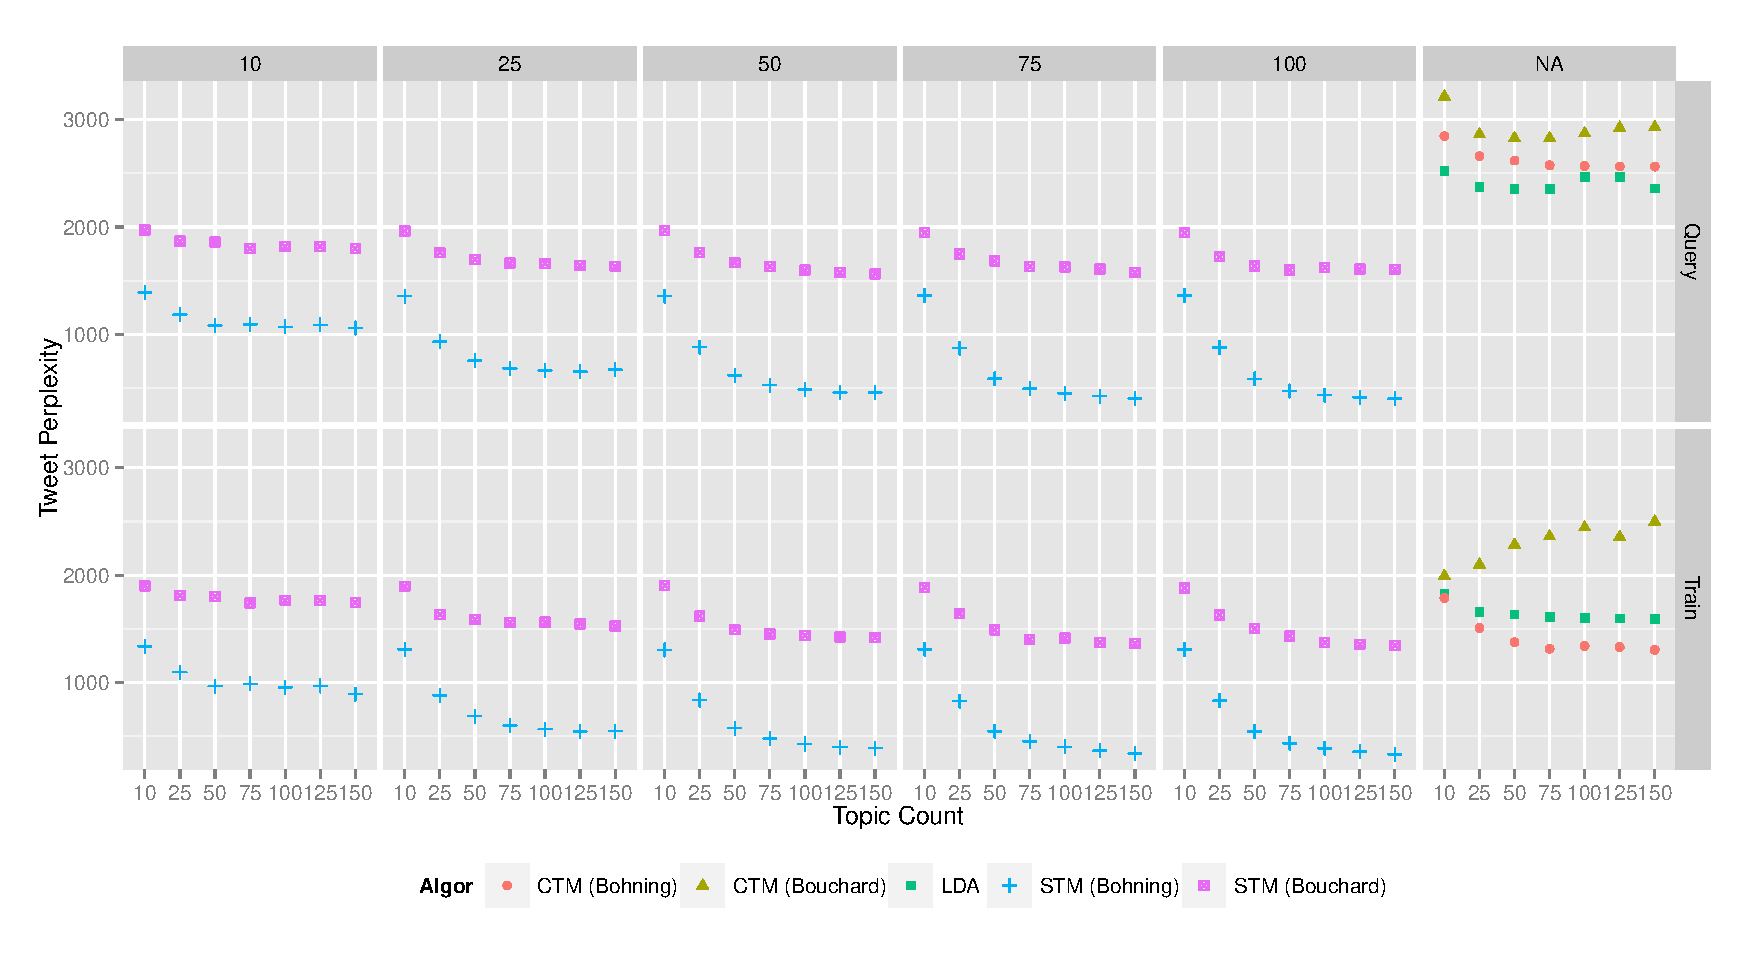
\includegraphics[width=0.95\textwidth]{Chap3/plots/tweet-all.eps}
    \caption{Performance of our model (STM), CTM, and LDA on the Tweets dataset, broken down by size of latent dimension, which is {\tt NA} for the CTM and LDA Author topic-model}
    \label{fig:tweet-all}
\end{figure}

\begin{figure}
\centering
    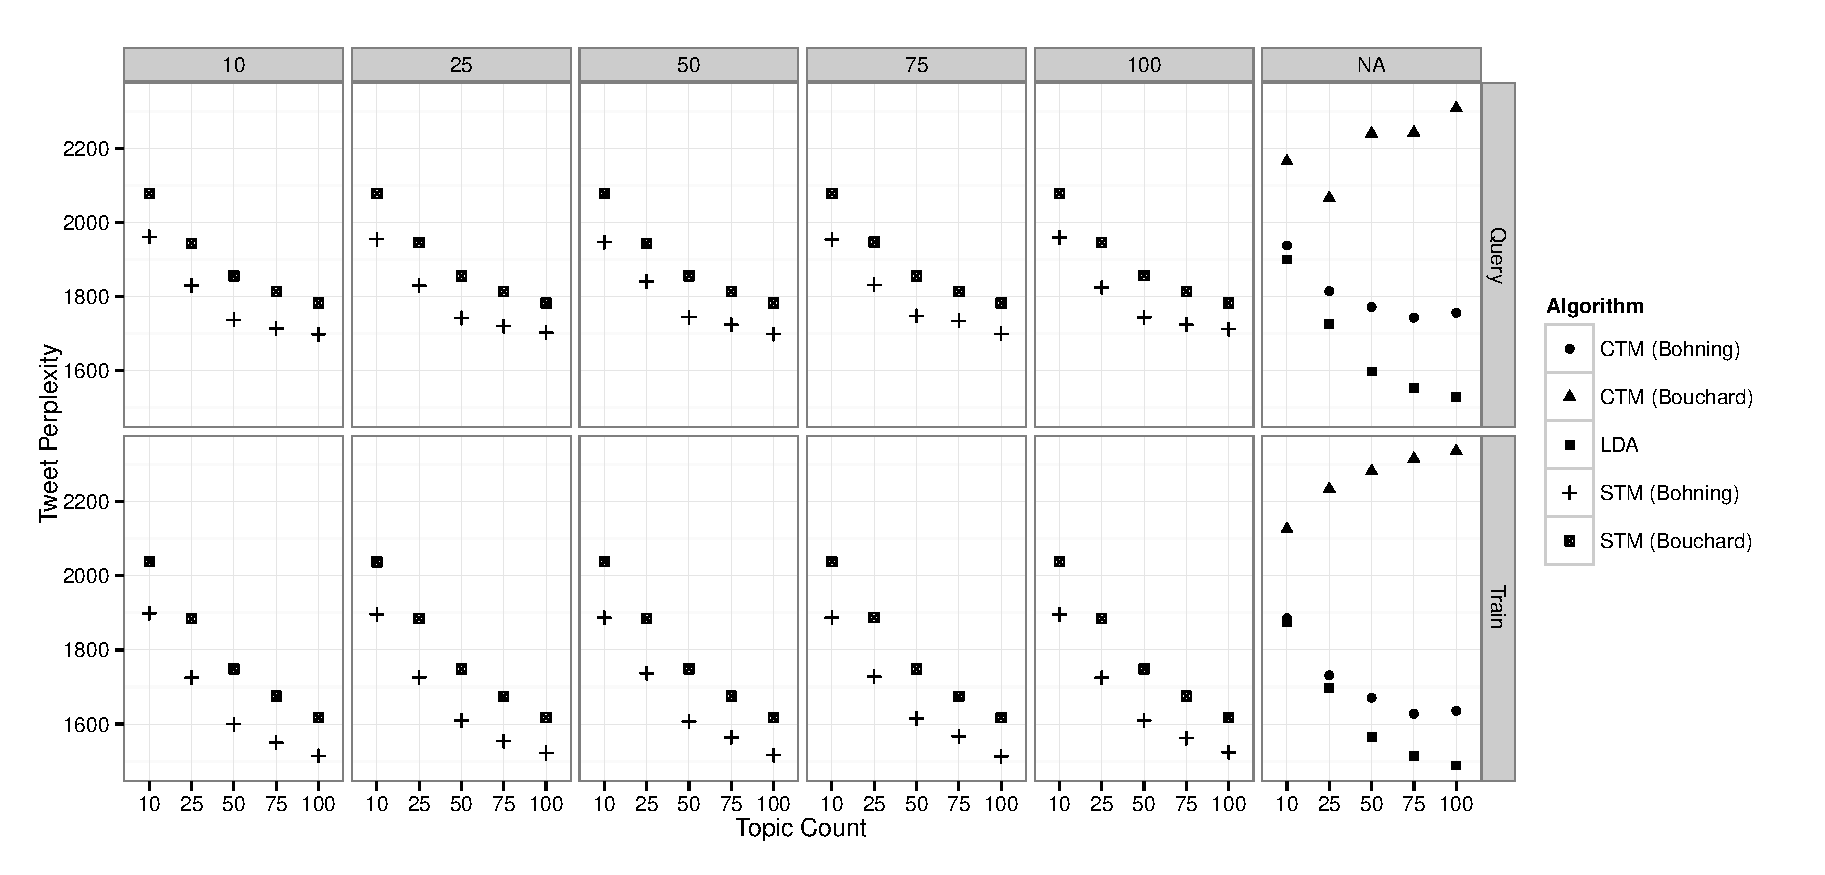
\includegraphics[width=0.95\textwidth]{Chap3/plots/acl-all.eps}
    \caption{Performance of our model (STM), CTM, and LDA on the ACL dataset, broken down by size of latent dimension, which is {\tt NA} for the CTM and LDA topic-models}
    \label{fig:acl-all}
\end{figure}

\begin{table}
    \centering
    \begin{tabular}{| l || p{9cm} | } \hline 
        \bf{Hashtag} & %\bf{User (Internal)} & 
        \bf{Tweet Words} \\ \hline
{\small \tt \#egypt} & 	{\small Egyptian street party \#tamarod \#june30 http://instagram.com/p/bU51EcHEBx/} \\ \hline
{\small \tt \#egypt} & 	{\small \#BREAKING: Clashes erupt between pro- and anti-Morsi crowds in Cairo http://f24.my/1cZMakS} \\ \hline
%{\small \tt \#syria} & 	{\small Gunfire and explosion heard from \#Nairobi \#WestgateMall as security forces push to end siege - http://aje.me/1dBkvsx} \\ \hline
{\small \tt \#news} &     {\small Cargill Invests \$200M in Volgograd Sunflower Oil Factory http://tmt-go.ru/484191 \#business} \\ \hline
{\small \tt \#syria} & 	{\small Syrian official blames rebels for purported chemical weapons attack near Damascus: http://apne.ws/19MMurk -DC} \\ \hline
{\small \tt \#news} & 	{\small Disgraced politician Bo Xilai hints at love triangle as trial ends in China: http://apne.ws/19IRzNQ -KH} \\ \hline
{\small \tt \#syria} & 	{\small UK-based watchdog says Syrian rebels shot down a fighter jet in \#Aleppo http://aje.me/11hGLG6} \\ \hline
{\small \tt \#syria} & 	{\small French intel says regime launched CW attack because it feared rebel offensive in Damas suburbs, wanted to protect Mezze military airport.} \\ \hline
{\small \tt \#craftbeer} & 	{\small Enjoying Southern Tier Brewing Co. Pumking Imperial Pumpkin Ale - 2013 using @brewvault. pic.twitter.com/yxJE7nBkcF} \\ \hline
{\small \tt \#gp3} & 	{\small Free Practice Results: http://www.gp2series.com/Results/ \#GP2 \#KeepCalmAndWin} \\ \hline
    \end{tabular}
    \caption{This table shows, for each hashtag, select tweets where that hashtag probability is above a threshold of 0.04 and the tweet itself lacks that hashtag. The preponderance of \hashtag{egypt} and \hashtag{syria} reflects active interests in 2013 (the ``Arab Spring").  }
    \label{tbl:generative}
\end{table}


\subsection*{ACL}
The results of running our model, and the CTM, and LDA topic models, on the ACL dataset are given in figure \ref{fig:acl-all}. The CTM (Bouchard) algorithm behaves similarly to the Twitter case. LDA, however, out-performs not only CTM, but also our model, in both training and query.

With such large documents (typically 3,000 words), the use of associated features such as author and year of publication evidently does not help, and merely hinders the inference of meaningful topics, compared to simply inferring topics directly from documents' words. Interestingly, the use of a correlated topic model also shows no benefit, even though there clearly is a sufficient number of documents to reliably infer a covariance matrix for the lower values of $K$. Inspection of the covariance matrix returned by the CTM (Bohning) model does show meaningful links between, for example, topics corresponding to different aspects of machine translation, but this information evidently does not aid model fit.

Clearly, in the presence of large documents, where all words associated with a topic occur in large numbers, there is no need for any ``transfer" of learning via a learnt covariance matrix, and features confer little advantage. Consequently, it is not surprising that the assumed rank of the feature-covariance, $P$, has little observable effect on the perplexity achieved by the STM models.


\begin{figure}
\centering     %%% not \center
\subfigure[ACL]{\label{fig:a}\includegraphics[width=60mm]{Chap3/plots/acl-cov-k25-k50-boh.pdf}}
\subfigure[Tweets]{\label{fig:b}\includegraphics[width=60mm]{Chap3/plots/tweets-cov-k25-k50-boh.pdf}}
\caption{Covariances over topics inferred using the Bohning implementation of the STM/YV model with $K=25$ and $P=50$}
\label{fig:acl-and-tweet-cov}
\end{figure}

\begin{table}
\begin{tabular}{| l | l | l | l | l | l | l | l |}
\hline
\specialcell{\small Parsing} &
\specialcell{\small Topic \\ Models} &
\specialcell{\small Machine \\ Translation} &
\specialcell{\small Kernel \\ Methods} &
\specialcell{\small Parts Of \\ Speech (POS)} &
\specialcell{\small Word-Sense \\ Disambiguation}\\
\hline
{\small pars} & 	{\small topic} & 	{\small align} & 	{\small kernel} & 	{\small tag} & 	{\small sens} \\
{\small grammar} & 	{\small model} & 	{\small word} & 	{\small tree} & 	{\small word} & 	{\small word} \\
{\small rule} & 	{\small word} & 	{\small model} & 	{\small featur} & 	{\small morpholog} & 	{\small us} \\
{\small tree} & 	{\small document} & 	{\small translat} & 	{\small us} & 	{\small us} & 	{\small disambigu} \\
{\small can} & 	{\small distribut} & 	{\small sentenc} & 	{\small structur} & 	{\small po} & 	{\small wordnet} \\
{\small parser} & 	{\small each} & 	{\small pair} & 	{\small can} & 	{\small languag} & 	{\small system} \\
{\small algorithm} & 	{\small us} & 	{\small english} & 	{\small svm} & 	{\small arab} & 	{\small wsd} \\
{\small from} & 	{\small our} & 	{\small us} & 	{\small learn} & 	{\small morphem} & 	{\small from} \\
{\small which} & 	{\small from} & 	{\small parallel} & 	{\small base} & 	{\small form} & 	{\small context} \\
\hline
\end{tabular}
\caption{Sample vocabularies for the ACL dataset from the the STM/YV model using the Bohning bound for $K=100$ and $P=50$. The unusual spelling is due to word-stemming}
\end{table}

\begin{table}
\begin{tabular}{| l | l | l | l | l | l |}
\hline
\specialcell{Tenns \\ {\small (R. Garros)}} &
\specialcell{Tennis \\ {\small (Wimbledon)}} &
\specialcell{US Politics \\ {\small(Liberal)}} &
\specialcell{US Politics \\ {\small(Republican)}} &
\specialcell{Beer \\ Enthusiasts} &
\specialcell{Markets} \\
\hline
{\small set} & 	{\small murrai} & 	{\small bill} & 	{\small obama} & 	{\small beer} & 	{\small morn} \\
{\small break} & 	{\small andi} & 	{\small white} & 	{\small fine} & 	{\small man} & 	{\small bui} \\
{\small point} & 	{\small draw} & 	{\small hous} & 	{\small gop} & 	{\small video} & 	{\small updat} \\
{\small serv} & 	{\small down} & 	{\small obama} & 	{\small listen} & 	{\small \#craftbeer} & 	{\small pleas} \\
{\small match} & 	{\small fact} & 	{\small american} & 	{\small hous} & 	{\small \#beer} & 	{\small sign} \\
{\small second} & 	{\small line} & 	{\small presid} & 	{\small experi} & 	{\small review} & 	{\small bank} \\
{\small up} & 	{\small set} & 	{\small program} & 	{\small republican} & 	{\small brew} & 	{\small perfect} \\
{\small winner} & 	{\small note} & 	{\small abort} & 	{\small senat} & 	{\small breweri} & 	{\small rais} \\
{\small hold} & 	{\small \#wimbledon} & 	{\small arriv} & 	{\small congrat} & 	{\small al} & 	{\small million} \\
{\small doubl} & 	{\small surpris} & 	{\small former} & 	{\small obamacar} & 	{\small nation} & 	{\small pt} \\
{\small \#rg13} & 	{\small tough} & 	{\small snowden} & 	{\small \#tcot} & 	{\small releas} & 	{\small initi} \\
{\small first} & 	{\small hewitt} & 	{\small west} & 	{\small stupid} & 	{\small fox} & 	{\small upgrad} \\
{\small from} & 	{\small 1st} & 	{\small nsa} & 	{\small immigr} & 	{\small craft} & 	{\small weather} \\
\hline
\end{tabular}
\caption{Sample vocabularies for the Twitter dataset from the the STM/YV model using the Bohning bound for $K=100$ and $P=50$. A peculiarity of Tweets is that we inferred several topics corresponding to different view-points of the same subject. The \hashtag{tcot} hashtag is an acronym of ``True Conservatives on Twitter"}
\end{table}


\section{Conclusion}
We have introduced a method employing multi-task learning to predict admixture-components, using quadratic bounds to overcome the non-conjugacy of the model. We have successfully applied this method in the case of a dataset of tweets: obtaining better model fit versus both simple and correlated author-topic models; and demonstrating the ability to employ this model as a query-expansion method for document retrieval. The use of the Bouchard bound failed to deliver any advantage in quality of model fit, and its rapid convergence in the initial iterations is not useful for priming the slower (in terms of iteration-count) Bohning bound algorithm.  Our method is not specific to any particularly dataset, and so can be applied to any dataset where features may be associated with observations which can be fit using an admixture model, though experiments suggest that, as outlined in the introduction, it is better suited to short and micro-texts where the use of a learnt prior can be motivated by a scarcity of words in each document.


%\begin{appendices}
%\chapter{The Variational Lower Bound}
%In this section we provide the variational lower-bound, or free-energy, for the two algorithms. This is taken after the bound has been applies to the likelihood.
%
%\section{Full-Covariance Model}
%The free-energy of the full-covariance bound is the sum of the terms given below.
%\begin{align}
%\begin{split}
%\ex{\ln p(Y)}{q} = &\halve{KP} \ln 2\pi - \halve{P}\ln |\Sigma| - \halve{KP}\ln \rho^2 - \half \Tr{\rho^{-2} \inv{\Sigma} M_Y M_Y\T}
%& \qquad + \half \Tr{S_Y\inv{\Sigma}\otimes R_Y \inv(\rho^{-2}I_P)}
%\end{split}
%\end{align}



%\chapter{Matrix Calculus Involving Kronecker Products}
%This briefly summarises the identities contained in three online resources\footnote{\url{http://research.microsoft.com/en-us/um/people/minka/papers/matrix/}}\footnote{\url{http://www4.ncsu.edu/~pfackler/MatCalc.pdf}}\footnote{\url{http://courses.engr.illinois.edu/cs598ps/CS598PS/Topics_and_Materials_files/Lecture\%201\%20-\%20Intro,\%20Linear\%20Algebra.pdf}} and then explains how these were used to take the derivatives of the expression
%
%\begin{equation}
%\Tr{A(X\T X \otimes Y\T Y) B}
%\end{equation}
%
%with respect to X and to Y.
%
%\section{Background}
%The definition of the Kronecker product and the $\vecf{\cdot}$ operator are assumed to be known. It is noted that in implementation terms, one can trivially implement the $\vecf{\cdot}$ operator using a \texttt{reshape} command, though only if the matrix is stored in column or ``Fortran" order. This is the case for Matlab, but most other numeric packages, including Numpy for Python, assume row or ``C" order. 
%
%Standard identites for Kronecker products and the related $\vecf{\cdot}$ operator are readily available\footnote{See for example ``The Matrix Cookbook" at \url{http://www2.imm.dtu.dk/pubdb/views/edoc_download.php/3274/pdf/imm3274.pdf}} but two of note are
%\begin{align}
%(X \otimes Y)\T & = X\T \otimes Y\T  \label{eqn:otimes_tranpose}\\
%\vecf{UXV} & = (V\T \otimes U)\vecf{X} \label{eqn:vec_to_otimes}
%\end{align}
%
%\subsection{The Vec-Transpose Operator}
%Both the $\vecf{\cdot}$ and tranpose operators can be generalized by the vec-transpose operator, introduced in \cite{Wandell1992}. This becomes a necessary tool when taking the derivatives of terms that occur in kronecker products.
%
%The vec-transpose of an $m \times n$ matrix $X$ is denoted $\vt{X}{p}$. The resulting matrix is composed of $n$ submatrices stacked atop one another, where each $p \times ^m/_p$ sub-matrix is generated by a fortran-order reshape of each column of X. The matrices are generated from top to bottom from the columns of X read from left to right. This is illustrated in the following examples.
%
%\begin{align}
%\begin{bmatrix} 
%    \color{Lavender}x_{11} & \color{CornflowerBlue}x_{12} \\
%    \color{Lavender}x_{21} & \color{CornflowerBlue}x_{22} \\
%    \color{Thistle}x_{31} & \color{RoyalBlue}x_{32} \\
%    \color{Thistle}x_{41} & \color{RoyalBlue}x_{42} \\
%    \color{Orchid}x_{51} & \color{Blue}x_{52} \\
%    \color{Orchid}x_{61} & \color{Blue}x_{62} 
%\end{bmatrix}^{(2)}
%= 
%\begin{bmatrix} 
%    \color{Lavender}x_{11} & \color{Thistle}x_{31} & \color{Orchid}x_{51} \\
%    \color{Lavender}x_{21} & \color{Thistle}x_{41} & \color{Orchid}x_{61} \\
%    \color{CornflowerBlue}x_{12} & \color{RoyalBlue}x_{32} & \color{Blue}x_{52} \\
%    \color{CornflowerBlue}x_{22} & \color{RoyalBlue}x_{42} & \color{Blue}x_{62} \\
%\end{bmatrix} \label{eqn:vt_example_2}
%\end{align}
%
%\begin{align}
%\begin{bmatrix} 
%    \color{Lavender}x_{11} & \color{CornflowerBlue}x_{12} \\
%    \color{Lavender}x_{21} & \color{CornflowerBlue}x_{22} \\
%    \color{Lavender}x_{31} & \color{CornflowerBlue}x_{32} \\
%    \color{Orchid}x_{41} & \color{NavyBlue}x_{42} \\
%    \color{Orchid}x_{51} & \color{NavyBlue}x_{52} \\
%    \color{Orchid}x_{61} & \color{NavyBlue}x_{62} 
%\end{bmatrix}^{(3)}
%= 
%\begin{bmatrix}
%    \color{Lavender}x_{11} & \color{Orchid}x_{41} \\
%    \color{Lavender}x_{21} & \color{Orchid}x_{51} \\
%    \color{Lavender}x_{31} & \color{Orchid}x_{61} \\
%    \color{CornflowerBlue}x_{12} & \color{NavyBlue}x_{42} \\
%    \color{CornflowerBlue}x_{22} & \color{NavyBlue}x_{52} \\
%    \color{CornflowerBlue}x_{32} & \color{NavyBlue}x_{62}
%\end{bmatrix}
%\end{align}
%
%The properties of the vec-transpose operator are:
%
%\begin{align}
%\vt{X}{1} & = X\T \\
%\vt{X}{\text{rows}(X)} & = \vecf{X} \\
%\vt{\vecf{X}}{r} & = \text{reshape(X,r,c)} & \text{\emph{(Fortran-order implementation)}} \\
%\vt{\vt{X}{p}}{p} & = X \label{eqn:a_pp_is_a} \\
%\vt{(aX + bY)}{p} & = a\vt{X}{p} + b\vt{Y}{p}
%\end{align}
%
%When working with traces, we can apply the vec-transpose operator inside the trace without affecting the result
%\begin{align}
%\Tr{X\T Y} = \Tr{\vt{(X)}{p}\T \vt{Y}{q}}
%\end{align}
%which generalizes the more commonly known identities
%\begin{align}
%\Tr{X\T Y} & = \vecf{X}\T\vecf{Y} \\
%\Tr{X\T Y} & = \Tr{X Y\T}
%\end{align}
%
%and in general we can apply any conformant reshaping, denoted with a a star, of the matrix dot-product within a trace without affecting the result
%\begin{align}
%\Tr{X\T Y} = \Tr{(X^*)\T Y^*} \label{eqn:tr_reshape}
%\end{align}
%
%{\color{red}An unproven result, verified empirically, is that for any matrix $X$ and appropriate values of $p$
%\begin{equation}
%    \left(\vt{X}{p}\right)\T \vt{I}{p} = \left(\vt{I}{p}\right)\T \vt{X}{p} \label{eqn:dot_of_vt_of_symmetric}
%\end{equation}
%}
%
%
%With these results in hand we can generalize equation \eqref{eqn:otimes_tranpose} as
%\begin{equation}
%\vt{(X \otimes Y)}{p} = X\T \otimes \vt{Y}{p} \label{eqn:vt_of_otimes}
%\end{equation}
%and equation \eqref{eqn:vec_to_otimes} as
%\begin{equation}
%\vt{\left((Z\T \otimes W)XY \right)}{p} = (Y \otimes W)\vt{X}{p}Z \label{eqn:extract_left_kro_opnd}
%\end{equation}
%where $p = \text{cols}(W)$.
%
%Crucially, this allows us to move the left operand, in this case $Z$, out of the kronecker product, enabling the use of standard identities to derive the derivative with respect to that operand.
%
%Using \eqref{eqn:extract_left_kro_opnd} we can show that
%\begin{equation}
%\vt{(\vt{(XY)}{p}Z)}{p} = (Z\T \otimes I)XY = \vt{(\vt{X}{p}Z)}{p}Y
%\end{equation}
%
%\subsection{The Commutation Matrix}
%In the previous section, we illustrated how we can swap-out the left-hand operand of a Kronecker product, enabling us to then apply the standard matrix-calculus identities. In this section we introduce the commutation matrix introduced in \cite{Magnus1988}, which allows us to swap the order of the operands in a kronecker product, moving the right-hand operand to the left from whence it can be swapped out subsequently using the vec-transpose operator.
%
%For an $m \times n$ matrix X, define the square matrix $T_{mn} \in \{0,1\}^{(m \times n) \times (m \times n)}$ that transforms $\vecf{X}$ into $\vecf{X\T}$:
%\begin{equation}
%T_{mn} \vecf{X} = \vecf{X\T}
%\end{equation}
%
%We can further define the matix $T_{nm}$ (note the order of the subscripts) such that
%\begin{align}
%T_{nm} T_{mn} \vecf{X}  & = \vecf{X} 
%\end{align}
%form which we can deduce the following three identities
%\begin{align}
%T_{nm} T_{mn}           &= I_{mn} \\
%T_{nm}                  &= \inv{T_{mn}} \\
%T_{mn}                  &= T_{nm}\T \label{eqn:transform_transpose}
%\end{align}
%
%Which taken together indicates that $T_{mn}$ is a square, orthogonal matrix. 
%
%These operators can be used to reorder the elements in a transpose. Assume X is an $m \times n$ matrix as before, and Y is a $k \times l$ matrix. Then
%\begin{align}
%Y \otimes X & = T_{km} (X \otimes Y) T_{nl} \label{eqn:kro_reorder} \\
%(X \otimes Y)T_{nl} & = T_{mk} (Y \otimes X)
%\end{align}
%Again, attention should be paid to the order of subscripts in the above results.
%
%Finally note that $T_{1m} = T_{m1} = I_m$. Hence, if for example X is a $1 \times n$ matrix then
%\begin{equation}
%(X \otimes Y)T_{nl} = Y \otimes X
%\end{equation}
%
%The elements of $T_{mn}$ are identified by the following equation, where $i \in [1\ldots mn]$ and $j \in [1 \ldots mn]$ are the row and column indices.
%\begin{equation}
%T_{mn}[i,j] = 
%\left\{
%    \begin{array}{lr}
%    1 & \text{if }  \left(j - \ceil{\frac{n}{i}}\right) \bmod n = 0 \\
%    0 & \text{otherwise}
%    \end{array}
%\right.
%\end{equation}
%
%
%\section{Connections between the Vec-Transpose Operator and Commutation Matrix}
%Looking at equation \eqref{eqn:vt_example_2}, where the vec-transform operator converts a $6 \times 2$ matrix into a $4 \times 3$ matrix, it is clear that no combination of square transformation matrices could achieve such a change in dimension, regardless of element ordering. Moreover $T_{mn}$ is explicitly defined in terms of the transform from $\vecf{X}$ to $\vecf{X\T}$
%
%Therefore rather than consider if one can express the vector-transform operator using commutation matrices, we must instead determine if a commutation matrix could be expressed in terms of the vec-transform operator.
%
%In short
%
%\begin{align}
%\mathcal{L}et\text{ } & \vv{x} = \vecf{X} & X \in \MReal{m}{n}\\
%\implies & T_{mn} \vv{x} = \vecf{X\T} \\
%\implies & T_{mn} \vv{x} = \vt{\vt{X}{1}}{n} \\
%\implies &\vt{\vt{\vt{\vv{x}}{m}}{1}}{n} = \vt{\vt{X}{1}}{n} \label{eqn:T_mn_to_vt}
%\end{align}
%
%Where in \eqref{eqn:T_mn_to_vt} we use \eqref{eqn:a_pp_is_a} to undo the $\vecf{\cdot}$ operation, then take the transpose via a vec-transpose operation, then re-apply $\vecf{\cdot}$ via another vec-transpose operation.
%
%Mathematically this is not a particularly useful result, replacing as it does one matrix multiplication with three applications of the vec-transpose operator. Programmatically, it is also likely that a sparse matrix-multiply is faster than several stacked \texttt{reshape} operations.
%
%\section{Derivatives of Terms in Kronecker Products}
%In this section we use the identities above, combined with standard matrix-calculus identities, to derive the derivative of
%
%\begin{equation}
%\Tr{A (X\T X \otimes Y\T Y) B}
%\end{equation}
%
%where $X \in \MReal{m}{n}$, $Y \in \MReal{k}{l}$, $A \in \MReal{nl}{a}$ and $B \in \MReal{nl}{b}$.
%
%\subsection{With Respect to the Left-Hand Operand}
%\newcommand \ddX  { \frac{d}{dX} }
%
%This proceeds in a straightforward manner, extending only slightly the example provided by Minka. 
%\begin{align}
%  & \ddX \Tr{A\T (X\T X \otimes Y\T Y) B} \\
%= & \ddX \Tr{\left(\vt{A}{l}\right)\T \vt{\left( (X\T X \otimes Y\T Y) B \right)}{l}} & \text{using } \eqref{eqn:tr_reshape} \\
%= & \ddX \Tr{\left(\vt{A}{l}\right)\T (I_{b} \otimes Y\T Y) \vt{B}{l} X\T X} & \text{using } \eqref{eqn:extract_left_kro_opnd} \\
%\begin{split}
%= & \quad X \left(\vt{A}{l}\right)\T (I_{b} \otimes Y\T Y) \vt{B}{l} \\
%  & \quad + X \left(\vt{B}{l}\right)\T (I_{b} \otimes Y\T Y) \vt{A}{l}  \label{eqn:lhs_kro_derivative}
%\end{split}
%\end{align}
%where in the final step we use the standard matrix-calculus result $\ddX \Tr{B X \T X} = XB + XB\T$. The scale of the vec-transporm operator is uniquely determined by conformability to be the number of columns in $Y\T Y$ which is $l$. If $A$ and $B$ are symmetric we can take advantage of \eqref{eqn:dot_of_vt_of_symmetric} to simplify the final result to
%\begin{equation}
%\ddX \Tr{A\T (X\T X \otimes Y\T Y) B} = 2X \left(\vt{A}{l}\right)\T (I_{b} \otimes Y\T Y) \vt{B}{l} \label{eqn:lhs_kro_derivative_symm_final}
%\end{equation}
%
%
%\subsection{With Respect to the Right-Hand Operand}
%This is much the same as before, except that we first employ two commutation matrices to re-arrange the order of the operands in the product.
%
%\begin{align}
%  & \ddX \Tr{A\T (X\T X \otimes Y\T Y ) B} \\
%= & \ddX \Tr{A\T T_{nl} (Y\T Y \otimes X\T X ) T_{ln} B} & \text{using }\eqref{eqn:kro_reorder} \\
%= & \ddX \Tr{ (T_{ln} A)\T (Y\T Y \otimes X\T X ) T_{ln} B} \text{using }\eqref{eqn:transform_transpose} \\
%= & \ddX \Tr{\left(\vt{(T_{ln} A)}{n}\right)\T \vt{\left( (Y\T Y \otimes X\T X ) T_{ln}B \right)}{n}} & \text{using } \eqref{eqn:tr_reshape} \\
%= & \ddX \Tr{\left(\vt{(T_{ln} A)}{n}\right)\T (I_b \otimes X\T X ) \vt{\left( T_{ln}B \right)}{n} Y\T Y } & \text{using } \eqref{eqn:extract_left_kro_opnd} \\
%\begin{split}
%= & \quad Y \left(\vt{(T_{ln} A)}{n}\right)\T (I_b \otimes X\T X ) \vt{\left( T_{ln}B \right)}{n} \\
%  & + Y \left(\vt{\left( T_{ln}B \right)}{n}\right)\T (I_b \otimes X\T X ) \vt{(T_{ln} A)}{n} \label{eqn:rhs_kro_derivative}
%\end{split}
%\end{align}
%
%The identity matrix in the kronecker produce is square with side equal to the columns of B. If B is square in turn, then the $I_b = I_{ln}$. {\color{red} TESTED BUT UNPROVEN. If A is symmetric and $B = I_{ln}$ then this simplifies to
%
%\begin{equation}
%\ddX \Tr{A\T (X\T X \otimes Y\T Y )} = 2 Y \left(\vt{(T_{ln} A)}{n}\right)\T (I_{ln} \otimes X\T X ) \vt{\left( T_{ln} \right)}{n} \label{eqn:rhs_kro_derivative_B_is_ident}
%\end{equation}
%}
%
%
%\end{appendices}
%



\

\newcommand \mnord[3] { { \mathcal{N}_{#1}\left({#2},{#3}\right) } }

\newcommand \const { { \text{c} } }

\providecommand \floor [1] { \left \lfloor #1 \right \rfloor }
\providecommand \ceil [1] { \left \lceil #1 \right \rceil }


\newcommand \vt[2] { { #1^{(#2)} } }

\newcommand \hashtag[1] { { \ttfamily \##1 } }

\newcommand \mvy  { \vv{m}_{\vv{y}} }
\newcommand \sigvy { { S_Y } }

\newcommand \mmy  { M_Y      }
\newcommand \md   { \vv{m}_d }
\newcommand \phin { \vv{\phi}_n }
\newcommand \isigma { { \inv{\Sigma} } }

\newcommand \sigv     { { \Sigma_V } }
\newcommand \isigv     { { \Sigma^{-1}_V } }

\newcommand \sigy { { \Sigma_Y } }
\newcommand \isigy { { \Sigma_{-1}_Y } }


\newcommand \omy  { { \Omega_Y } }
\newcommand \iomy { { \inv{\Omega_Y} } }

\newcommand \siga     { { \Sigma_A } }
\newcommand \isiga     { { \Sigma^{-1}_A } }
\newcommand \diagv { { \diag{\nu_1,\ldots,\nu_P} } }

\newcommand \ma { \vv{m}_a }
\newcommand \my { \vv{m}_y }

\newcommand \VoU { V \otimes U }

%\newcommand \one { \mathbb{1} }
\newcommand \one  {{  \mathds{1} }}

\newcommand \lse { \text{lse} }
%\newcommand \lse[0] { \mathrm{lse} }

% Conditional independence
\def\ci{\perp\!\!\!\perp} % from Wikipedia



% ------ For the eval section

% Multinomial PDF [Math Mode]
% params: 1 - the variable
%         2 - the value
%         3 - the state indicator (e.g. k for a distro with K values)
%         4 - any additional subscript
\newcommand{\mpdf}[4] {
	\prod_{#3} {#1}_{{#4} {#3}} ^ {#2}
}

% Dirichlet PDF [Math Mode]
% params: 1 - the variable
%         2 - the hyper-parameter
%         3 - the state indicator (e.g. k for a distro with K values)
%         4 - any additional subscript
\newcommand{\dpdf}[4] {
	\frac{1}{B({#2})} \prod_{#3} {#1}_{{#4} {#3}} ^ {({#2}_{#3} - 1)}
}

% To simplify the sampling equations, this is indicates
% that the given value has had datapoint "m" stripped out
%
\newcommand{\lm}[1] {
	#1^{\setminus m}
}

\newcommand \model[0] {
    \mathcal{M}
}

\newcommand \perplexity[1] {
    \mathcal{P} \left( { #1 } \right)
}

\newcommand \WTrain {
    \mathcal{W}^{(t)}
}

\newcommand \WQuery {
    \mathcal{W}^{(q)}
}

\newcommand \oneover[1] {
    \frac{1}{ {#1} }
}

\newcommand \samp[1] {
    { #1 }^{(s)}
}

\newcommand \etd[0] {
    \vv{\eta}_d
}

\newcommand \Ed {{ \vv{\xi}_d}}
\newcommand \Edj {{\xi_{dj}}}
\newcommand \Edk {{\xi_{dk}}}
\newcommand \AEdj {{\Lambda(\xi_{dj})}}
\newcommand \AEdk {{\Lambda(\xi_{dk})}}
\newcommand \AEd  {{ \bm{\Lambda}(\bm{\xi}_d) }}

\newcommand \Axi { { \Lambda_{\xi} } }
\newcommand \bxi { { \vv{b}_{\xi} } }
\newcommand \cxi { { c_{\xi} } }

\chapter{Jointly-Low Rank Admixture Models}
In the previous chapter, we investigated a correlated admixture model which employed low-rank projections of features in order to derive parsimonious model representations. A weakness of that model is that we increase the number of topics for a fixed dataset, there is a risk that the model becomes overparameterised once more: in particular the correlation matrix over topics may become singular.

In this chapter we provide an inference algorithm which enabled both low-rank feature \emph{and} topic covariance matrices. Standard application of the mechanics of variational inference would lead to an algorithm whose computational complexity was $O(P^3Q^3)$ where $P << F$ and $Q << K$ are the dimensions of our low-rank projections of the $F\times F$ covariance matrix over features and $K \times K$ covariance matrix over topics. We derive a novel algorithm instead whose computational complexity of $O(P^3 + Q^3)$, making inference in this model feasible.

\section{The Jointly Low-Rank Model}

The scenario is the same as in the previous chapter: features $\vv{x}_d$ with associate short texts $\wdoc$. We seek to assign topics to documents, so as to perform query expansion on them.

This is achieved by altering the manner in which we make predictions in the previous "YV" model to the following:

\begin{align}
Y \sim & \mnord{QP}{0}{\rho^2 I_P}{\alpha^2 I_Q} & A|Y \sim & \mnord{KF}{UYV\T}{\alpha^2 I_F}{\sigma^2 I_K} \\
\thd | A \sim & \nor{\axd}{\sigma^2 I_K}
\end{align}

Unfortunately, we can no longer obtain a matrix-variate marginal distribution over A, and so must use the multi-variate density to describe the marginal distribution.  

\begin{align}
\vecf{A} \sim \nor{\vv{0}}{\alpha^2 \sigma^2 I_{FK} + \rho^2 V\T V \otimes \tau^2 U\T U}
\end{align}

We refer to this as the reduced-covariance model.

\subsection{Variational Inference}
One approach to the reduced covariance model is to attempt to use matrix-variate posteriors with separate covariances -- $q(Y) \sim \mnord{QP}{M_Y}{R_Y}{S_Y}$, $q(A) \sim \mnord{KF}{M_A}{R_A}{S_A}$ --  despite the non-separability of the marginalized prior. However this immediately leads to a Sylvester equation, indicating that the covariance of the variational posterior is non-separable.

\begin{align}
\vecf{M_Y} = & \invb{\rho^{-2}\tau^{-2} I_{PQ} + \alpha^{-2}V V\T \otimes \sigma^{-2} U \T U}\vecf{\sigma^{-2}\alpha^{-2} U\T M_A V\T}
\end{align}

Collecting terms it's clear our approximate posterior over Y is a multivariate normal distribution over $\vecf{Y}$: $q(Y) = \nor{\vv{m}_y}{S_y}$. Using this we can recalculate the expectations of the affected terms in the free-energy

\begin{align}
\ex{p(Y)}{q} = & -\halve{PQ}\left(\ln 2\pi + \ln \rho^2 + \ln \tau^2\right) - \half \left(\rho^{-2}\tau^{-2} \vv{m}_y\T\vv{m}_y + \Tr{\rho^{-2}\tau^{-2} S_Y}\right) \\
\begin{split}
\ex{p(A|Y)}{q} = & -\halve{FK}\left(\ln 2\pi + \ln \rho^2 + \ln \tau^2\right) \\
 & -\half \Tr{\alpha^{-2}\sigma^{-2}(M_A - U M_Y V)(M_A - U M_Y V)\T} \\
 & -\half \Tr{S_Y \left(\alpha^{-2}V V\T \otimes \sigma^{-2}U \T U\right)} \\
 & -\half \Tr{\sigma^{-2}S_A\otimes \alpha^{-2}R_A}
 \label{eqn:free_enery_u_and_v}
\end{split}
\end{align}

Basic calculus gives us an update for Y

\begin{align}
S_y & = \invb{\rho^{-2} \alpha^{-2} I_{PQ} + V\T V \otimes U\T U}
&
\vv{m}_y & = S_y \vecf{U M_A V}
\end{align}

Unfortunately this requires inverting $S_y \in \mathbb{R}^{(P \times Q) \times (P \times Q)}$. This has a computational complexity of $O(P^3Q^3)$ which is not tractable. Therefore we develop the following method to reduce the computational complexity to $O(P^3 + Q^3)$ by analytically deriving the update for $Y$ from the eigen-decompositions of $U\T U$ and $V\T V$..

Recall that the eigen-decomposition of a matrix V is $U_V D_V U_V\T$ where $U$ is the matrix of V's eigen-vectors and $D$ a diagonal matrix of its eigen-values. The inverse is $\inv{V} = U_V \inv{D_V} U_V\T$, where the inverse of $D_V$, being diagonal, is trivially obtained. It has been shown in \cite{Stegle2011} that if $A = (a I + C \otimes B)$ then the eigen-decomposition is
\begin{align}
A = (a I + C \otimes B) = (U_C \otimes U_B)(\alpha I + D_C \otimes D_B)(U_C\T \otimes U_B\T)
\end{align}

We use this in our update for $\vv{m}_y = \vecf{M_Y}$. For brevity we use the change of notation $\vecf{U M_A V} = \vecf{T}$ and additionally denote the eigen-decompositions $U\T U = U_U D_U U_U\T$ and $V\T V = U_V D_V U_V\T$, given the revised update:

\begin{align}
\vecf{M_Y} = (U_V \otimes U_U)
  \invb{\alpha^{-2}\rho^{-2} I + S_V \otimes S_U}
  (U_V^\top \otimes U_U^\top) \vecf{T}
\end{align}

We can simplify this further. Letting $S = (\alpha^{-2}\rho^{-2} I + D_V \otimes D_U)$, we can define a second term $s$ according to

\begin{align}
S^{-1}(U_V^\top \otimes U_U^\top) \vecf{T} 
& =
(U_V^\top \otimes U_U^\top)S^{-1} \vecf{T} \\
& =
\vecf{U_U (\text{diag}(S^{-1})^{(Q)} .* T) U_V^\top} = s
\end{align}

where $.*$ denotes the Hadamard product, and we use the notation $A^{(p)}$ to denote the vec-transpose\cite{Minka2000a}. Further information on the vec-transpose operator is given in the appendix (section \ref{sec:vec-transpose} but not that $\vecf{A}^{(Q)} = \text{reshape}(A, rows=Q, cols=c)$.

Using the identity $\vecf{AXB} = (B\T \otimes A)\vecf{X}$ we can now re-write

\begin{align}
\vecf{M_Y} = (U_V \otimes U_U)s = \vecf{U_U^\top s^{(Q}) U_V}
\end{align}

Removing the vec operator from both sides and expanding terms we arrive at the final update for $Y$

\begin{align}
Y = U_U^\top (\diag{\inv{S}}^{(Q)} .* (U_U U M_A V U_V^\top)) U_V
\end{align}

\subsubsection{Inferring U and V}
The inference of U and V requires being able, in both cases, to differentiate the term

\begin{align}
\Tr{(V\T V \otimes U\T U)S_y} \label{eqn:kro-deriv-input}
\end{align}
which appears in the expectation of $\ex{\ln p(A)}{q}$.

As described in \cite{Minka2000a} taking derivates of Kronecker products involves the introduction of a \emph{commutation matrix} $T_{QP}$, a square, orthogonal, permutation matrix defined by the property that $T_{QP} \vecf{X} = \vecf{X\T}$. The derivatives of \eqref{eqn:kro-deriv-input} are (with apologies for the abuse of notation):

\begin{align}
\frac{d}{dU} \Tr{(V\T V \otimes U\T U)S_y} 
& = \left( \vt{(T_{QP} S_y)}{P} \right)\T (I_{PQ} \otimes V\T V)\vt{T_{QP}}{P}
\\
\frac{d}{dV} \Tr{(V\T V \otimes U\T U)S_y} 
& = \left(\vt{S_y}{Q}\right)\T (I_{PQ} \otimes U\T U) \vt{I_{PQ}}{Q}
\end{align}
The full derivation of these two results is given in the appendix, section \ref{sec:trace-kro-calculus}


\subsubsection{Inferring Document Level Topics}
Taking the derivates of the free-energy and setting to zero provides the following update for the distribution of topics for document $d$

\begin{align}
\md = & \invb{\sigma^{-2}I_K + N_d \Axi} \left(\sigma^{-2} M_A \xd  + N_d \bxi + Z^{(d)}\vv{w}_d \right )
\end{align}

As in the Low+Full model, this ostensibly involves a matrix inverse for every document, however by expanding terms and employing the Sherman-Morrison identity we can actually obtain the inverse analytically.

\begin{align}
\invb{\sigma^{-2}I_K + N_d \Axi}
& = \invb{(\sigma^{-2} + \halve{N_d})I_K + \frac{N_d}{2K + 2} \mathbf{1} \mathbf{1}\T} \\
& = \invb{a_d I_K + b_d \mathbf{1}\mathbf{1}\T} \\
& = \inv{a_d} I_K - \frac{{a_d}^{-2}b_d }{1 + \inv{b_d}K}\mathbf{1}\mathbf{1}\T
\end{align}

This provides an extremely efficient inference scheme. The full set of updates is given in algorithm \ref{alg:uyv}.

\newcommand \mvy  { \vv{m}_{\vv{y}} }
\newcommand \sigvy { { S_Y } }

\newcommand \mmy  { M_Y      }
\newcommand \omy  { \Omega_Y }
\newcommand \sigy { \Sigma_Y }

\subsection*{Matrix Calculus for Kronecker Products}
Solving for $U$ and $V$ requires the use of the vec-transpose \emph{operator} introduced in \cite{Wandell1992} and the \emph {communtation matrix} introduced in \cite{Magnus1988}. These are described here.

The vec-transpose of an $m \times n$ matrix $X$, denoted by $\vt{X}{p}$ is composed of $n$ submatrices stacked atop one another, where each $p \times ^m/_p$ sub-matrix is generated by a fortran-order reshaping of each column of X. The matrices are generated from top to bottom from the columns of X read from left to right. It generalizes both the transpose and $\vecf{\cdot}$ operations, as $\vt{X}{1} = X\T$ and $\vt{X}{\text{rows}(X)} = \vecf{X}$.

For an $m \times n$ matrix X, the commutation matrix is the square permutation matrix $T_{mn} \in \{0,1\}^{(m \times n) \times (m \times n)}$ that transforms $\vecf{X}$ into $\vecf{X\T}$ such that:
\begin{equation}
T_{mn} \vecf{X} = \vecf{X\T}
\end{equation}

With these we can define the following identities for the differentiation of terms in both sides of a Kronecker product. For the purpose of these identities only let $A \in \MReal{a}{nl}$, $X \in \MReal{m}{n}$ and $Y \in \MReal{k}{l}$ and thereby define

\begin{align}
\begin{split}
\frac{d}{dX} \Tr{A\T(X\T X \otimes Y\T Y)} & = 2X \left(\vt{A}{l}\right)\T (I_{nl} \otimes Y\T Y) \vt{I_nl}{l} \label{eqn:lhs_kro_derivative_symm}
\end{split} \\
\begin{split}
\frac{d}{dY} \Tr{A\T(X\T X \otimes Y\T Y)} & = 2 Y \left(\vt{(T_{ln} A)}{n}\right)\T (I_{nl} \otimes X\T X ) \vt{\left( T_{ln} \right)}{n} \label{eqn:rhs_kro_derivative_B_is_ident}
\end{split}
\end{align}

The vec-transpose operator and the commutation matrix and their applications to calculus are explained in more detail in \cite{Minka2000a}. The appendix provides a summary of the key points, and the derivations of \eqref{eqn:lhs_kro_derivative_symm} and \eqref{eqn:rhs_kro_derivative_B_is_ident}.

\subsection*{Derivation of the updates for U and V}

Starting first with V, we can use \eqref{eqn:lhs_kro_derivative_symm} to take the derivative of \eqref{eqn:free_enery_u_and_v} and so derive the following solution

\begin{equation}
V = \invb{\mmy\T U\T U \mmy + \left(\vt{S_Y}{Q}\right)\T (I_{PQ} \otimes U\T U) \vt{I_{PQ}}{Q} } \sigma^{-2} M_A \T U \mmy
\end{equation}

Next, for U, we employ \eqref{eqn:rhs_kro_derivative_B_is_ident} which provides the solution:
\begin{equation}
U = \invb{\mmy V\T V \mmy\T + \left( \vt{(T_{QP} S_Y)}{P} \right)\T (I_{PQ} \otimes V\T V)\vt{T_{QP}}{P}} M_A V \mmy\T
\end{equation}

Standard matrix calculus provide solutions for $\vv{m}_y $ and $S_Y$
\begin{align}
S_Y = & \invb{I_{mn} + V\T V \otimes U\T U}
& \vv{m}_y = & S_Y \vecf{U\T M_A V}
\end{align}


\begin{algorithm}
\caption{Representing $A=UYV$}
\label{alg:uyv}
$\text{ }$\\
{\bf E-Step}
    \begin{align*}
        & S_y = \invb{I_{mn} + V\T V \otimes U\T U} \quad &
Y & = U_U^\top (\diag{\inv{S}}^{(Q)} .* (U_U U M_A V U_V^\top)) U_V \\
        & &
        S & = (\alpha^{-2}\rho^{-2} I + D_V \otimes D_U) \\
        & S_A = \sigma^2 I_K \quad R_A = \invb{\alpha^{-2} I_F + \sigma^{-2} X\T X} 
        & M_A & = \left(\alpha^{-2} YV + \sigma^{-2} \sum_d \md \xd\T\right)R_A
    \end{align*}
    \begin{align*}
         \Vd = & \invb{\sigma^{-2}I_K + N_d \Axi}\\
         \md = & \invb{\sigma^{-2}I_K + N_d \Axi} \left(\sigma^{-2} M_A \xd  + N_d \bxi + Z^{(d)}\vv{w}_d \right )\\
        \gamma_{dvk} \propto & \beta_{kv} e^{m_{dk}} 
\end{align*}
{\bf M-Step}
\begin{align*}
    U = & \invb{\mmy V\T V \mmy\T + \left( \vt{(T_{QP} S_Y)}{P} \right)\T (I_{PQ} \otimes V\T V)\vt{T_{QP}}{P}} M_A V \mmy\T \\
    V = & \invb{\mmy\T U\T U \mmy + \left(\vt{S_Y}{Q}\right)\T (I_{PQ} \otimes U\T U) \vt{I_{PQ}}{Q} } M_A \T U \mmy \\
    \beta_{kv} \propto & \sum_d z_{dvk} w_{dv} 
\end{align*}
{\bf Bohning Bound M-Step}
    \begin{align*}
        \Axi & = \half \left(I_K - \mathbf{1}_K\mathbf{1}_K\T / K  \right) \\
        \bxi & = \Axi \vv{m}_d  - \sigma{\vv{m}_d}
    \end{align*}
\ref{alg:yv}
\end{algorithm}



\section{Experiments}
\begin{figure}
  \centering
    \hspace*{-1.5cm}\includegraphics[height=0.25\textheight]{./Chap5/plots/figs/Fig5.png}
  \caption{Comparison between our model (``Corr-UYV") and other commonly used models}
  \label{fig:uyv-fig}
\end{figure}

In this section, we present an evaluation of all three mod-
els on 7000 images and captions from the Corel database. We held out 25\% of the data for testing purposes and used the remaining 75\% to estimate parameters. Each image is segmented into 6-10 regions and is associated with 2-4 caption words. The vocabulary contains 168 unique terms. We used the InceptionV3 neural network to extract features from the image in the dataset.

Our baseline was the GM-LDA model\cite{Blei2003} which uses a link-function to infer topic-strengths given simple LDA assignments.

\subsection{Test set likelihood }
To evaluate how well a model fits the data, we computed
the per-image average negative log likelihood of the test set on all three models for various values of K. A model which better fits the data will assign a higher likelihood to the test set (i.e., lower numbers are better in negative likelihood). Figure 5 illustrates the results. As expected, GM-LDA provides a much better fit than GM-Mixture.Further-more, Corr-LDA provides as good a fit as GM-LDA.This is somewhat surprising since GM-LDA is a less constrained model. However, both models have the same number of parameters; their similar performance indicates that, on aver- age, the number of hidden factors used to model a particular image is adequate to model its caption.

\subsection{Automatic annotation}
Given a segmented image without its caption, we can use
the mixture models described in Section 3 to compute a
distribution over words conditioned on the image, p(w| r). This distribution reflects a prediction of the missing caption words for that image.

To measure the annotation quality of the models, we com-
puted the perplexity of the given captions under $p(w| x)$ for each image in the test set. Perplexity,


Figure \ref{fig:uyv-fig} (Left) shows the perplexity of the held-out captions under the maximum likelihood estimates of each model for different values of K. We see that overfitting is a serious problem in the GM-Mixture model, and its perplexity immediately grows off the graph (e.g., when K = 200, the perplexity is 2922). Note that in related work, many of the models considered are variants of GM-Mixture and rely heavily on an ad-hoc smoothing procedure to correct for overfitting. Figure \ref{fig:uyv-fig} (Right) illustrates the caption perplexity under
the smoothed estimates of each model using the empirical Bayes procedure. The overfitting of GM- Mixture has been corrected. Once smoothed, it performs better than GM-LDA despite the GM-LDA model’s superior performance in joint likelihood. We found that GM-LDA does not provide good conditional distributions for two reasons. First, it is ``over-smoothed." Computing $p(w| x)$ requires integrating a dif- fuse posterior (due to the small number of regions) over all the factor dimensions. Thus, the factors to which each region is associated are essentially washed out and, as K gets large, the model’s performance approaches the performance of the simple maximum likelihood estimate of the caption words.

\begin{figure}
  \centering
    \hspace*{-1.5cm}\includegraphics[height=0.40\textheight]{./Chap5/plots/figs/Fig2.png}
  \caption{Sample annotations for various images}
  \label{fig:uyv-fig}
\end{figure}

Second, GM-LDA easily allows caption words to be generated by factors that did not contribute to generating the image regions (e.g., when K = 200, 54\% of the caption words in the test set are assigned to factors that do not appear in their corresponding images). With this freedom, the estimated conditional Gaussian parameters do not necessarily reflect regions that are correctly annotated by the corresponding conditional multinomial parameters. While it better models the joint distribution of words and regions, it fails to model the relationship between them. Most notably, Corr-LDA finds much better predictive
distributions of words than either GM-LDA or GM-Mixture. It provides as flexible a joint distribution as GM-LDA but guarantees that the latent factors in the conditional Gaussian (for image regions) correspond with the latent factors in the conditional multinomial (for caption words). Furthermore, by allowing caption words to be allocated to different factors, the Corr-LDA model achieves superior performance to the GM-Mixture which is constrained to associating the entire image/caption to a single factor. Thus, with Corr-LDA, we can achieve a competitive fit of the joint distribution and find superior conditional distributions of words given images

Figure \ref{fig:uyv-images} shows ten sample annotations—the top five words
from $p(w|x)$ computed by each of the three models for K = 200. These examples illustrate the limitations and
power of the probabilistic models described in Chapter 1 when used for a practical discriminative task

The GM-LDA model, as shown quantitatively in the previous section, gives the least impressive performance of the three. First, we see washing out effect described above by the fact that many of the most common words in the corpus — words like “water” and “sky” — occur in the predicted captions for all of the pictures. Second, the predicted caption rarely predicts the object or objects that are in the picture. For example, it misses “jet” in the picture captioned clouds, jet, plane, a word that both other models predict with high accuracy. The GM-Mixture model performs better than GM-LDA, but we can see how this model relies on the average image features and fails to predict words for regions that may not generally occur in other similar images. For example, it omits “tree” from the picture captioned scotland, water since the trees are only a small part on the left side of the frame. Furthermore, the GM-Mixture predicts completely incorrect words if the average features do not easily correspond to a common theme. For example, the background of fish, reefs, water is not the usual blue and GM-Mixture predicts words like “fungus”, “tree”, and “flowers.” Finally, as reflected by the term perplexity results above,
the Corr-LDA model gives the best performance and correctly labels most of the example pictures. Unlike the GM- Mixture model, it can assign each region to a different cluster and the final distribution over words reflects the ensemble of clusters which were assigned to the image regions. Thus, the Corr-LDA model finds the trees in the picture labeled scotland, water and can correctly identify the fish, even without its usual blue background.

\section{Conclusion}
We have presented a novel method, with fast, efficient inference, for incorporating features into topics. Our method avoids the issues of singular matrices that occur when estimating large covariance parameters from few parameters. Our method also, it should be said, provides the basis for a fast, efficient, two-dimensional PCA algorithm.

A disadvantage of our method is the need to determine the latent dimensions in advance. In practice, in our results, this was obtained by grid-search, but this is highly time-consuming.

Nevertheless, our model provides a useful means for augmenting existing image captioning schemes.

\

\newcommand \thdo { { \vv{\theta}_{d\cdot} } }
\newcommand \thok { { \vv{\theta}_{\cdot k} } }
\newcommand \phok { { \vv{\phi}_{\cdot k} } }
\newcommand \phdo { { \vv{\phi}_{d\cdot} } }

\chapter{Correlated Admixture Models for Relational Document Networks}
In this section we apply the framework of correlated admixtures of text with covariates to the problem of relational learning. In particular we examine relational learning within document networks. Typically approaches to this problem have focussed on simply the presence of links between documents. We go one step further and assign an \emph{incidence} to each link, being the number of times it was cited in a source document.

We build on our previous work with correlated topic models with covariates, and previous published work on using paired admixture models jointly on document words and document links, to derive a novel model, with fast efficient inference, which can model link presence and suggest new links for existing documents.
\section{Introduction}
This is concerned with the predictions of which papers should be cited by an origin paper - very similar to a recommendation system. For brevity the ``source" paper in the network is the \emph{paper}, and the destination paper is the "reference". So we are concerned with how to predict the references for a paper, particularly references which have not been included in the dataset. If we restrict ourselved to the ACL dataset, we have author, year, venue, title and full-text for both papers and references.

Previous work on link prediction for academic papers has suggested\cite{Bethard2010} that the most influential factors when choosing references: whether the reference is a self-citation; whether it is a self-citation one step removed (e.g. Alice cites a paper by Bob who's previously cited Alice); how often a paper is cited a priori; the terms of the paper; how old the cited paper in relative terms; whether the cited and citing papers shared a venue; and finally functions of the topics inferred from the words using LDA\cite{Blei2003}.

Many other approaches have used topics, often in a multiview setting. In some cases a function of the distance between two topics is learnt\cite{Chang2009a}\cite{Chang2010a}, but the linkage structure reveals topics not evident in the text, leading some to adapt the topics of a paper when it is a ``destination" by adding in some learnt document-specific noise\cite{Neiswanger2014} and the FIXME POISSON paper.

A different arrangement possible when one has text for papers and references is the LDA/PLSA model\cite{Nallapati2008}\cite{Nallapati2008a} in that the topics used to generate links differ to those used to generate words, though both share the same Dirichlet prior. In the LDA/PLSA model, it's assumed one has the words of the linked to documents, and that the $K \times L$ matrix distribution of per-topic link-distributions can be used as $L \times K$ matrix of per-link topic-distributions used to model the linked documents' words. Sharing the parameter allows a transfer of learning from the words of the linked documents to the generation of links in linking documents.
The only other paper, aside from \cite{Bethard2010}, to consider time is \cite{Gerrish2010} which builds on the dynamic topic model of \cite{Blei2006a} in which time was quantized, and per-topic vocabularies changed between quanta according to a Kalman Filter style algorithm operating on the logistic-normal vocabulary distributions. The novel aspect is in the addition of an impact factor, one for each paper and topic, which upweights the contribution of that paper's topic-words when inferring the prior over vocabularies in the next time-step. This model limited itself solely to text and did not consider linkage structure.

Link prediction is an unbalanced prediction problem, with very few positive examples in the dataset. In the case of \cite{Bethard2010} a variant of SVM optimising the MAP criterion\cite{Yue2007} (i.e. ranking) was found to outperform logistic regression and logistic regression with downsampled negative inputs. In the RTM model\cite{Chang2009a}\cite{Chang2010a} a single-class classifier was trained, regularised by using a combination of Gaussian priors and the addition of a number of pseudo-documents for the negative case drawn from the posterior, their number indicated by means of a parameter $\rho$. This was motivated by the fact that the absence of links cannot be construed as evidence indicating links should not exist, and therefore one should not employ the ``zeroes" in the dataset as negative samples when training a classifier. Other approaches have simply ignored the imbalance, or in the case of the Link-PSLA-LDA model\cite{Nallapati2008}\cite{Nallapati2008a} used a multinomial distribution over documents' out-links, whose posterior is a function solely of existing links (the ``ones").


\section{The Model}
Following the example of the correlated topic model (CTM)\cite{Blei2006} we try to capture correlations between topics. We collect the individual document topic-score vectors $\thdo$ into a matrix $\Theta \in \MReal{D}{K}$. 
\begin{align}
\Theta &\sim \mnor{\vv{\mu}\one\T}{\Sigma}{\alpha I_D}
\end{align}

Denoting the softmax function as $\sigma_k(\vv{\theta}) = \frac{\theta_k}{\sum_j \theta_j}$ and the vector of softmax scores as $\vv{\sigma}(\vv{\theta})$ we 
the topic for the $n$-th of the $N^w_d$ words in document $d$ as
\begin{align}
\zdn & \sim \muln{\vv{\sigma}(\thdo)}{1} &
\wdn & \sim \muln{\vv{\lambda}_{z_{dn}}}{1}
\end{align}
And likewise for the $m$-th of the $N^l_d$ out-links in document $d$
\begin{align}
y_{dm} & \sim \muln{\vv{\sigma}(\thdo)}{1} &
l_{dp} & \sim \muln{\vv{\beta}_{- z_{dn}}}{1}
\end{align}

Were we to put simple Dirichlet priors over $\vv{\beta}_k$ and $\vv{\phi}_k$ we would just have a simple multi-field (or ``multi-modal") topic-model\cite{Salomatin2009}. However we instead wish to transfer our knowledge of how topics are emitted by document $\Theta$ to the parameter $\Phi = \{ \vv{\phi}_k\T \}_{k=1}^K$ governing how documents are emitted for each topic $k$. Thus we use the following prior:
\begin{align}
\Phi|\Theta & \sim \mnor{\Theta}{\Sigma}{\diag{\vv{\rho}}}
\end{align}
where $\vv{\rho} \in \VReal{D}$ is the column covariance of all documents. 

\section{Inference with Non-Conjugate Bounds}
\subsubsection*{The Matrix-Normal Distribution}
Given a random matrix $X \in \MReal{D}{K} \sim \mnor{M}{\Sigma}{\Omega}$ with row covariance $\Sigma \in \MReal{K}{K}$ and column covariance $\Omega \in \MReal{D}{D}$ its log-pdf is given by
\begin{align}
\halve{DK}\ln 2\pi - \halve{D}\ln|\Sigma| - \halve{K} \ln|\Omega| -\Tr{\inv{\Omega}(X - M)\inv{\Sigma}(X - M)\T}
\end{align}
This is mathematically identical to the following distribution over the vectorized matrix X, $\vecf{X} \sim \nor{\vecf{M}}{\Omega \otimes \Sigma}$. It should be noticed that this approach, due to the assumed separability of the covariance, is a considerably more parsimonious model than naively assuming $\vecf{X} \sim \nor{\vecf{M}}{S}$. The separability assumption, i.e. that $S = \Omega \otimes \Sigma$ means that the covariance is approximated in the following ways:

\begin{align}
\cov{X_{dk}, X_{pj}} & = \Omega_{dp} \Sigma_{kj} &
\cov{X_{d-}} & = \Omega_{dd} \Sigma &
\cov{X_{-k}} & = \Sigma_{kk} \Omega \label{eqn:sep-cov-forms}
\end{align}

\subsubsection*{Non-Conjugate Bounds}
The log-probability of the emission probabilities for words is given by
\begin{align}
\ex{p(Z)}{q} = \sum_d \sum_n \sum_k \zdnk \ex{\thdk}{q} - \sum_d N^w_d \text{ }\ex{\lse(\thdo)}{q}
\end{align}
where the log-sum-exp function is $\lse(\thd) = \ln (\sum_k e^\thdk)$. As this expectation cannot be evaluated analytically, we choose to bound it with an analytically tractable expression. While Taylor series expansions have been used the past\cite{Blei2006}\cite{Wang2013a}, these involve iterating though Newton-Raphson steps which are both computationally expensive and lack convergence guarantees. Therefore we use the Bohning bound approximation\cite{Bohning1988} which is both guaranteed to converge, and has a quadratic form that allows for closed form updates.

The bound is given by
\begin{align}
\lse(\thdo) \leq \half \thdo\T A_K \thdo - \vv{b}_d\T\thdo + c_d \label{eqn:lse-def}
\end{align}
where
\begin{align}
A_K & = \half \left( I_K - \frac{1}{K} \one \one\T \right) \\
b_d & = A_K \Ed - \vv{\sigma}(\Ed) \label{eqn:bohning-b} \\
c_d & = \frac{1}{2} \Ed\T A_K \Ed - \vv{\sigma}(\Ed)\T\Ed + \lse(\Ed) \label{eqn:bohning-c}
\end{align}

Employing this bound, and denoting $N^o_d = N^w_d + N^l_d$ we can lower-bound the log probability of the emission topics as

\begin{equation}
\begin{aligned}
\ex{p(X,Y)}{q} & \geq \sum_d  (\sum_n \vv{z}_{dn} + \sum_m \vv{y}_{dm}) \ex{\thdo}{q} \\
   & - \sum_d N^o_d \left(\half \ex{\thdo}{q}\T A_K \ex{\thdo}{q} - \vv{b}_d\T\ex{\thdo}{q} + c_d\right)
\end{aligned}
\end{equation}

Taking derivatives of the complete log-likelihood and solving for zero, we see that the solution to the bound parameter is $\Ed = \ex{\thdo}{q}$. 

Substituting $\ex{\thdo}{q}$ for $\Ed$ in \eqref{eqn:bohning-b} and \eqref{eqn:bohning-c} we see that equation \eqref{eqn:lse-def} simplifies to $\ex{\lse(\thdo)}{q} \leq \lse(\ex{\thdo}{q})$ which is equivalent to a zero-order Delta method approximation (i.e. a zero-order Taylor series approximation around $\ex{\thdo}{q}$). However the use of the longer, quadratic form avoids the need for a nested iterative inference scheme such as Newton-Raphson in determining the posterior mean of $\thdo$.

Similarly, the distribution over out-links can be bounded as

\begin{align}
\ex{p(L|Y)}{q} & \geq \sum_p \sum_m \sum_k \sum_d y_{pmk} l_{pmd} \ex{\phi_{dk}}{q} \\
 & - \sum_p \sum_m \sum_k \sum_d y_{pmk} l_{pmd} \left(\half \ex{\phok}{q}\T A_D \ex{\phok}{q} - \vv{f}_k\T \ex{\phok}{q} + g_k\right)
\end{align}
where the bound parameter in this case $\vv{\xi}_k = \ex{\phok}{q}$. Letting $\hat{L}_{dk} = \sum_p \sum_m y_{pmk} l_{pmd}$ and the diagonal matrix $N^i = \diag{\sum_d \hat{L}_{d\cdot}}$, we can see that $N^i$ is the diagonal matrix of how often an \emph{``in-link"} is generated by topic $k$. With this notation we can write:
\begin{align}
p(L|Y) & \geq \sum_k \hat{L}_{\cdot k}\T \ex{\phok}{q} - \sum_k N^i_{kk} \left(\half \ex{\phok}{q}\T A_D \ex{\phok}{q} - \vv{f}_k\T \ex{\phok}{q} + g_k\right) \\
& = \ex{\Tr{L \Phi}}{q} - \half \ex{\Tr{A_D \Phi N^i \Phi}}{q} + \ex{\Tr{F \Phi}}{q} - \one\T G \one \\
& = \sum_d \hat{L}_{d\cdot} \phdo - \half \sum_{p \neq d} A_{dp} \vv{\phi}_{p\cdot}\T N^i \phdo -\half A_{dd} \phdo\T N^i \phdo + F_{d\cdot}\T\phdo + G_{d\cdot}
\end{align}
where the matrices $F \in \MReal{D}{K}$ and $G \in \MReal{D}{K}$ simply collect the vectors $\vv{f}_k$ and $\vv{g}_k$. This gives us a lower bound, which we denote $\hat{p}(\Theta, Z, Y, W, L, \Phi)$  on the complete probability


\subsubsection*{Variational Inference}
Having lower-bounded the complete log likelihood using Bohning's bound, we can then employ an approximate posterior distribution $q(\Theta, Z, Y, \Phi, \Sigma, \vv{\rho}, \alpha)$ in conjunction with Jensen's to obtain a lower-bound on the marginal log-likelihood:

\begin{align}
\ln p(W, L) \geq \ex{\hat{p}(\Theta, Z, Y, W, L, \Phi)}{q} - \ent{q}
\end{align}

We use the following mean-field factorisation
\begin{align}
q(\Theta, Z, Y, \Phi, \Sigma, \vv{\rho}, \alpha) = q(\alpha)q(\Sigma)\prod_d q(\thd)q(\vv{\phi}_d)q(\rho_d)\prod_n q(\vv{z}_{dn})q(\vv{y}_{dn}).
\end{align}

In most cases, the posterior is naturally conjugate to the prior and likelihood, and the parameter estimates are easily obtained. However, the cases of the topic-distribution matrix $\Theta$ and the document-emission matrix $\Phi$ require special attention. The obvious choice in each case is a matrix-variate posterior distribution, however while one can obtain a multivariate Normal posterior over $\vecf{\Theta}$, the covariance of that distribution is not separable into a Kronecker product of two matrices, and thus no matrix-variate posterior over $\Theta$ exists. A similar issue arises with $\Phi$. Thus we take the aggressive form of the mean-field factorisation outlined above where we consider the rows of the matrices individually.

\newcommand \mtd { { \vv{m}^{\theta}_d } }
\newcommand \std { { S^\theta_d } }
\newcommand \mpd { { \vv{m}^{\phi}_d } }
\newcommand \spd { { S^\phi_d } }

\begin{align}
q(\Theta) &= \prod_d \mathcal{N}\left(\thdo; \mtd, \std \right) &
q(\Phi) &= \prod_d \mathcal{N}\left(\phdo; \mpd, \spd\right) 
\end{align}
and further assume that the covariances $\std$ and $\spd$ are diagonal. Denoting the sum of expected topic assignments for document $d$ as $\hat{\vv{z}}_{d\cdot} = \sum_n \ex{\vv{z}_{dn}}{q}$ and $\hat{\vv{y}}_{d\cdot} = \sum_m \ex{\vv{y}_{dm}}{q}$ we obtain the following updates for both means:
\begin{align}
\mtd &= \invb{ \invb{(\alpha + \rho_d)\Sigma} + N^o_d A_K }
            \left(
                \invb{\rho_d \Sigma} \mpd
                + \invb{\alpha \Sigma}\vv{\mu}
                + \vv{b}_d 
                + \hat{\vv{z}}_{d\cdot}
                + \hat{\vv{y}}_{d\cdot}
            \right) \\
 \mpd & = \invb{\invb{\rho_d \Sigma} + A_{dd}N^i}
             \left(
                 \invb{\rho_d \Sigma}\mtd + N^i F_{d\cdot} -\half \sum_{p \neq d} A_{dp} N^i \vv{m}^\phi_p + \hat{L}_{d\cdot}
             \right)
 \end{align}
 
As can be expected, both updates feature as the first term of the right-hand side the value of the (full) posterior covariance matrix. In both cases the posterior precision is a sum of two terms each of which takes the form of a scalar inverse variance times a precision matrix, as one would expect given the matrix-variate form. 

In the case of $\mtd$, the matrix $A_K$ is a component of the posterior row-precision and the matrix $N^o = \diag{N^o_1, \ldots, N^o_D}$ is a component of the column precisoin. In the case of $\mpd$ these roles are reversed, due to the bound operating column-wise. Note that $A_{dd} = \frac{D-1}{2D}$ while $A_{dp} = - \oneover{2D}$

The interpretation of these two distributions is that $q(\thd)$ is the distribution of document $d$ being the \emph{origin} of a word or link according to topic $k$, whereas $q(\vv{\phi}_d)$ is the distribution of a document being the \emph{target} of a link emitted according to topic $k$.

\begin{algorithm}
\caption{Matrix-Variate Topic Model}
\label{alg:sra_generic}

    \begin{align*}
        \mtd &= 
            \invb{ \invb{(\hat{\alpha} + \hat{\rho}_d)\hat{\Sigma}} + N^o_d A_K } \\
            & \times \left(
                \invb{\hat{\alpha} \hat{\Sigma}}\vv{\mu}
                + \invb{\hat{\rho}_d \hat{\Sigma}} \mpd + \vv{b}_d 
                + \sum_n \ex{\vv{z}_{dn}}{} 
                + \sum_m \ex{\vv{y}_{dn}}{}
            \right)\\
         S^\theta_{d,kk} &= \invb{\inv{\hat{\alpha}} + \inv{\hat{\rho}_d} + \inv{\hat{\Sigma}}_{kk}} \\
         \mpd & = \invb{\invb{\hat{\rho}_d \hat{\Sigma}} + A_{dd}N^i} \\
             & \times \left(
                 \invb{\hat{\rho}_d \hat{\Sigma}}\mtd 
                 + N^i F_{d\cdot} 
                 -\half \sum_{p \neq d} A_{dp} N^i \vv{m}^\phi_p 
                 + \hat{L}_{d\cdot}
             \right) \\
        S^\phi_{d,kk} & = \invb{ \inv{\hat{\rho}_d} \inv{\hat{\Sigma}_{kk}} + A_{dd}N^i_{kk} } \\
        z_{dnk} & \propto \exp(\ex{\theta_{dk}}{q})\beta_{k,w_{dn}} \\
        y_{dmk} & \propto \exp(\ex{\theta_{dk}}{q} + \ex{\phi_{l_{dp},k}}{q}) \\
        \vv{\beta}_{kt} & = \sum_d \sum_n \sum_t \ex{z_{dnk}}{q} w_{dnt} \\
        \ex{\Sigma}{q} & =  \oneover{\nu + 2D} \left(\Sigma_0
             + \sum_d \inv{\ex{\alpha}{}} (\mtd - \vv{\mu})(\mtd - \vv{\mu})\T + \std  \right .\\
            & \qquad\qquad\qquad\quad+ \left. \sum_d \inv{\ex{\rho_d}{}} (\mpd - \mtd)(\mpd - \mtd)\T + \spd \right)  \\  \ex{\rho_d}{} & = \oneover{a + K} \left(b + (\mpd - \mtd)\T \inv{\hat{\Sigma}} (\mpd - \mtd) + \Tr{\std \inv{\hat{\Sigma}}} + \Tr{\spd \inv{\hat{\Sigma}}} \right) \\
        \ex{\alpha}{q} & = \oneover{a + DK} \left(b + \sum_d (\mtd - \vv{\mu})\T\inv{\hat{\Sigma}}(\mtd - \vv{\mu}) + \Tr{\std \inv{\hat{\Sigma}}} \right) \\
        \vv{\mu} &= \oneover{D} \sum_d \mtd
    \end{align*}
    For brevity, we let $\hat{\alpha} = \ex{\alpha}{}$, $\hat{\rho}_d = \ex{\rho_d}{}$ and $\hat{\Sigma} = \ex{\Sigma}{}$
\end{algorithm}

\subsubsection*{Non-Identifiability of the prior Covariances}
Careful attention needs to be applied to the case of the prior covariances: factors in Kronecker products are inherently non-identifiable as $A \otimes B = c A \otimes \frac{1}{c} B$ for any constant $c$. In practice this means that maximum likelihood estimates of A and B can diverge below and over machine precision respectively.

In the case of maximum likelihood estimation this is addressed by means of ``flip-flop" algorithms\cite{Srivastava2009} which fix an element of one matrix to a constant value and adjust the other accordingly. In our case, take a Bayeisan approach and put priors over the covariances, drawing $\alpha$ and $\rho_d$ from the same inverse-gamma prior $\inv{\Gamma}\left(a, b\right)$ and $\Sigma \sim \inv{\mathcal{IW}}\left(\Sigma_0, \nu\right)$. 


\subsubsection*{Eliminating topic assignments}
Storing $z_{dnk}$ and $y_{dmk}$ for every word or link in every document is prohibitively difficult. Therefore in our implementation we simply substitute the update for these variables in those terms where they appear, and simplify. This significantly improves the runtime of our algorithm. 
\section{Experiments}

\begin{figure}
  \centering
    \hspace*{-1.5cm}\includegraphics[height=0.40\textheight]{./Chap6/plots/RPlot.pdf}
  \caption{Results of our model on the ACL corpus dataset}
  \label{fig:chap5-fig-self-1}
\end{figure}

The dataset is the Associated for Computational Linguistics (ACL) corpus of academic papers. Each document has associated with it a list of links to other documents in the corpus, the list of authors, the venue and the year published. Additionally we have extracted the number of times each out-link occurs in the paper text. \emph{(We also have the surrounding text, but we don't use it)}.

To prepare the data, we remove all documents with fewer than three unique words, which leaves 13,533 documents. Then, from that, we remove document with fewer than 2 out-links. This results in a corpus of 4,264 documents. The total word-count of that corpus is 14,864,709 words drawn from a dictionary of 23,769 unique terms.

The evaluation methodology consists of removing from each document half of its links, training on the full corpus, and then evaluating the rank of the held out links.

We use three ranking metrics metrics. Mean reciprocal-rank, is the average of the reciprocal of the ranks of all held-out links across all documents: $mrr = \frac{1}{D} \sum_d \frac{1}{Q} \sum_q r_q$.  


\begin{figure}
  \centering
    \hspace*{-1.5cm}\includegraphics[height=0.33\textheight]{./Chap6/plots/figs/fig-1.png}
  \caption{Comparison between our model (``MTM") and other commonly used models}
  \label{fig:chap5-fig-compare-2}
\end{figure}

The precision at m is the precision evaluated on the top-ranked $m$ documents, which is simply the quotient of the number of held-out links found in that subset and $m$. The recall at m similarly is the recall evaluated on the top-ranked $m$ documents, being the quotient of number of held-out links returned and either $m$ or the total number of out links that could be returned, whichever is smaller. Precision and recall at m were averaged across all documents in the corpus. In all cases larger values are better.

As a model convergence check, we also look at the perplexity of the words and links. This is the marginal log-likelihood normalized by document length, according to 

\begin{equation}
\mathcal{P}erp(W,L) = \exp\left( - \frac{\ln p(W,L)}{\sum_d N^w_d + N^l_d} \right)
\end{equation}
Smaller perplexity scores are better.


The baseline models currently consist of the RTM model, which as established earlier, performs extremely poorly, and a previous version of this model, ``MTM-Old" which re-used $\Theta$ for link emissions
\begin{align}
\Theta & \sim \mnor{0}{I}{\Sigma} &
z_{dn} & \sim \muln{\vv{\sigma}(\thdo)}{1} &
w_{dn} & \sim \prod_k \muln{\vv{\beta}_k}{1}^{z_{dnk}} \\
& &
y_{dm} & \sim \muln{\vv{\sigma}(\thdo)}{1} &
l_{dp} & \sim \prod_k \muln{\vv{\sigma}(\thok)}{1}^{y_{dmk}}
\end{align}
As noted in previous work, MTM-Old exhibits the property that the model prefers to adapt $\Theta$ to fit words rather than out-links, which is unsurprising since each document has approximate 300 words for every out-link. Consequently, as training progressed for that model, perplexity scores improved while recall and precision scores degraded. The current model, where the emission distribution for links $\Phi$ is separate from $\Theta$ seeks to address this.

We used weak priors for the variances, with $a = b = 0.001$, and $\nu = 1.1 \times K$ and $\Sigma_0 = 0.001 I_K$.

The results for precision and recall at M are given in tables \ref{tbl:rtm}, \ref{tbl:mtm-old} and \ref{tbl:mtm-new}. The documents are grouped into subsets based on how many out-links they have. This is the ``group" column with the number of documents in each group in the ``count" column.

The mean reciprocal-rank for 25 topics for RTM, MTM-Old and MTM-New is are 0.0016, 0.0887 and 0.1050 respectively.

The perplexity for 25 topics for RTM, MTM-Old and MTM-New as evaluated on the \emph{training} dataset is 1581.67, 1559.38 and 15.68 respectively. I just use this as a convergence check. The old MTM model does a better job of modelling words and links despite doing worse at ranking, but in reality it's simply focusing on words which outnumber links 300 to 1.

\begin{table}{\small
Precision at m\\
\begin{tabular}{| l | r || c | c | c | c | c | c | c | c | c |}\hline
 Group    & Count &    10 &    20 &    30 &    40 &    50 &    75 &   100 &   250 &   500  \\
\hline
  0,    3 &      2460 & 0.000 & 0.000 & 0.000 & 0.000 & 0.000 & 0.000 & 0.000 & 0.001 & 0.000  \\
  3,    5 &       634 & 0.000 & 0.000 & 0.001 & 0.001 & 0.001 & 0.001 & 0.001 & 0.001 & 0.001  \\
  5,   10 &       546 & 0.000 & 0.000 & 0.000 & 0.001 & 0.001 & 0.001 & 0.001 & 0.002 & 0.002  \\
 $\geq 10$ &        86 & 0.001 & 0.001 & 0.001 & 0.002 & 0.002 & 0.002 & 0.002 & 0.003 & 0.003  \\
\hline\end{tabular}\\

Recall at m\\
\begin{tabular}{| l | r || c | c | c | c | c | c | c | c | c |}\hline
 Group    & Count &    10 &    20 &    30 &    40 &    50 &    75 &   100 &   250 &   500  \\ \hline
  0,    3 &      2460 & 0.001 & 0.003 & 0.006 & 0.010 & 0.010 & 0.014 & 0.017 & 0.078 & 0.124  \\
  3,    5 &       634 & 0.000 & 0.002 & 0.004 & 0.009 & 0.010 & 0.013 & 0.016 & 0.060 & 0.102  \\
  5,   10 &       546 & 0.000 & 0.001 & 0.002 & 0.006 & 0.006 & 0.011 & 0.013 & 0.052 & 0.111  \\
 $\geq 10$ &        86 & 0.001 & 0.001 & 0.002 & 0.007 & 0.008 & 0.010 & 0.013 & 0.051 & 0.112  \\
\hline\end{tabular}
\caption{Precision and recall at m for the RTM model with 25 topics. Mean reciprocal rank is 0.0016}\label{tbl:rtm}
}\end{table}

\begin{table}{\small
Precision at m\\
\begin{tabular}{| l | r || c | c | c | c | c | c | c | c | c |}\hline
 Group    & Count &    10 &    20 &    30 &    40 &    50 &    75 &   100 &   250 &   500  \\
\hline
  0,    3 &      2460 & 0.032 & 0.022 & 0.017 & 0.015 & 0.013 & 0.010 & 0.009 & 0.005 & 0.003  \\
  3,    5 &       634 & 0.081 & 0.053 & 0.042 & 0.036 & 0.032 & 0.025 & 0.021 & 0.012 & 0.007  \\
  5,   10 &       546 & 0.121 & 0.080 & 0.065 & 0.056 & 0.049 & 0.039 & 0.033 & 0.020 & 0.012  \\
 $\geq 10$ &        86 & 0.208 & 0.142 & 0.112 & 0.096 & 0.083 & 0.066 & 0.056 & 0.033 & 0.021  \\
\hline\end{tabular}\\

Recall at m\\
\begin{tabular}{| l | r || c | c | c | c | c | c | c | c | c |}\hline
 Group    & Count &    10 &    20 &    30 &    40 &    50 &    75 &   100 &   250 &   500  \\ \hline
  0,    3 &      2460 & 0.180 & 0.239 & 0.288 & 0.332 & 0.365 & 0.434 & 0.491 & 0.695 & 0.832  \\
  3,    5 &       634 & 0.181 & 0.237 & 0.283 & 0.324 & 0.356 & 0.421 & 0.479 & 0.673 & 0.829  \\
  5,   10 &       546 & 0.168 & 0.221 & 0.269 & 0.311 & 0.338 & 0.403 & 0.457 & 0.675 & 0.823  \\
 $\geq 10$ &        86 & 0.165 & 0.225 & 0.264 & 0.300 & 0.325 & 0.388 & 0.441 & 0.646 & 0.815  \\
\hline\end{tabular}
\caption{Precision and recall at m for the old MTM model with 25 topics. Mean reciprocal rank is 0.0887}\label{tbl:mtm-old}
}\end{table}

\begin{table}{\small
Precision at m\\
\begin{tabular}{| l | r || c | c | c | c | c | c | c | c | c |}\hline
 Group    & Count &    10 &    20 &    30 &    40 &    50 &    75 &   100 &   250 &   500  \\
\hline
  0,    3 &      2460 & 0.045 & 0.031 & 0.024 & 0.020 & 0.017 & 0.013 & 0.010 & 0.005 & 0.003  \\
  3,    5 &       634 & 0.113 & 0.079 & 0.061 & 0.050 & 0.043 & 0.032 & 0.026 & 0.012 & 0.007  \\
  5,   10 &       546 & 0.155 & 0.113 & 0.092 & 0.077 & 0.066 & 0.051 & 0.041 & 0.020 & 0.012  \\
 $\geq 10$ &        86 & 0.245 & 0.179 & 0.147 & 0.124 & 0.108 & 0.083 & 0.068 & 0.033 & 0.019  \\
\hline\end{tabular}\\

Recall at m\\
\begin{tabular}{| l | r || c | c | c | c | c | c | c | c | c |}\hline
 Group    & Count &    10 &    20 &    30 &    40 &    50 &    75 &   100 &   250 &   500  \\ \hline
  0,    3 &      2460 & 0.253 & 0.348 & 0.403 & 0.441 & 0.476 & 0.535 & 0.571 & 0.680 & 0.772  \\
  3,    5 &       634 & 0.258 & 0.356 & 0.412 & 0.448 & 0.481 & 0.534 & 0.576 & 0.689 & 0.791  \\
  5,   10 &       546 & 0.215 & 0.316 & 0.381 & 0.425 & 0.458 & 0.526 & 0.567 & 0.692 & 0.795  \\
 $\geq 10$ &        86 & 0.193 & 0.283 & 0.348 & 0.394 & 0.427 & 0.492 & 0.535 & 0.659 & 0.766  \\
\hline\end{tabular}
\caption{Precision and recall at m for the current MTM model with 25 topics. Mean reciprocal rank is 0.1050}\label{tbl:mtm-new}
}\end{table}

\subsubsection*{Model Variants}
We have presented a model which links the emission of topics per document, to the emissions of documents per topic, and therefore shares information between these two related tasks. \\

Our model is the first, to our knowledge, which uses the \emph{incidence} rather than mere \emph{existence} of links when modelling relationships between documents. It avoids the quadratic scaling problem of \cite{Chang2009a} and instead uses a deterministic inference algorithm which is linear in the number of links.\\

Our model can be used to predict links for existing and new documents, in the latter case by inferring $\thdo$ from document words. Our ranking results, on existing documents is competitive with published work, notably \cite{Chang2009a}\cite{Neiswanger2014} and we are actively experimenting with implementations of competing models and other datasets.



\

\chapter{Conclusions and Future Work}
In this chapter we enumerate the main contributions of this thesis. We discuss the challenges that remain, and outline further avenues of research which may be promising.

\section{Contributions}
This thesis has concerned itself with the intersection of four areas of research which have hitherto been kept separate: analysis of text with mixture \& admixture models; multi-task learning with learnt priors; and marginalisation and dimensionality reduction in observations with matrix-variate distributions.

As a motivating example, we have focussed on short and ``micro" texts, where due to low word-counts, it may not be possible to obtain good \emph{predictive} performance with traditional mixture models. 

We have made a number of advances. First, we have shown that for admixture models derived from the correlated topic-model\cite{Blei2006}, the Bohning bound provides the best convergence and speed guarantees, contrary to the existing published literature\cite{Wang2013}. We have provided an algorithm taking advantage of parallelisable instructions which in addition to providing best of class performance in terms of predictive quality; also provides best of class performance in terms of execution time.

Building on this improvement on the CTM, we have developed a model for incorporating covariates which takes into account the latent structure that exists between covariates, in a multi-task framework, to provide improved predictive ability. We have demonstrated empirically the advantage that this provides over simpler models\cite{Mimno2008}, and shown how it may be a useful adjunct to existing deep-learning networks for image classification, providing a means to perform both query expansion and aid classification on heavily unbalanced datasets.

As a part of this work we have developed a novel new algorithm for inference on matrix-variate distributions, which provides the basis for an efficient double-PCA algorithm on matrix-variate distributions.


\section{Future Work}
There are nevertheless a number of gaps in our work. The most significant is the need to perform exhaustive grid searches to determine the number of topics and latent dimensions.

In the case of the Dirichlet distribution, the Dirichlet process and the Pitman-Yor Process both allow the data to determine the number of components. 

For logistic-normal prior, the discrete, infinite, logistic normal (DILN) model\cite{Paisley2012b} similarly provides a non-parametric equivalent. It is formed by combining a gamma-process to determine partition probabilities (analogous to using the gamma distribution to sample from a Dirichlet), then using a Gaussian process to capture correlations between such partitions. Since the covariance kernel of a Guassian process will consume too much memory for all but the most trivial of datasets, a covariance \emph{matrix} is measured in practice corresponding to a linear kernel between observations.

For incorporation into our model, we would need to prove two identities: the first, that a separable covariance matrix with a Kronecker structure corresponds to a valid kernel function; and secondly that the resulting infinite-dimensional normal distribution is equivalent to a matrix-variate normal distribution. If feasible, this would also admit non-parametric inference of the number of components in Principal Components Analysis.

It is also obvious that the distributions used to model vocabularies are sub-optimal in our model. This was a conscious decision, as the focus of the work was in deriving novel priors over topic distributions. Nevertheless, given the extreme Zipfian nature of the vocabulary of tweets in particular, we should seek to use a Pitman-Yor Process to model the vocabulary, which has been shown to exhibit good performance in past work\cite{Buntine2014}. Further improvements such as burst models are perhaps less important given our decision to blend topics using correlation. For tweets in particular, this model is a poor fit, since it does not generalise to new users: this leads to a representation problem of how to represent Twitter users from their ancillary information.

This could be combined with a stochastic inference algorithm to improve convergence. Using natural gradients, the updates should not need to change.

The most intriguing extension is outside the scope of this thesis. As an example use-case, we combined our model with a deep-neural network for feature extraction. While classic neural network literature\cite{Bishop2006} uses the softmax function for activation functions, more recent practitioners have used an unbouned $\exp(.)$ function to avoid the vanishing gradients problem. This was attempted before in the Dirichlet Multinomial Regression model\cite{Mimno2008}. This suggests that we could use Dirichlet distribution to generate discrete outputs, and stack them as in the Pachinko Allocation model\cite{Li2006}. Being Dirichlet, one could further investigate the use of non-parameteric extensions to handle the number of internal layers.



\clearpage
$\text{ } $
\clearpage
$\text { }$
\clearpage
$\text { }$
\bibliographystyle{plain}
\bibliography{/Users/bryanfeeney/Documents/library.bib}

\end{document}


